% VedGraph: Agentic Construction of an Evidence-Typed Knowledge Graph
% for the Vedic Samhitas
%
% Build:  tectonic -X compile main.tex
% Fonts:  Libertinus (free, shipped with TeX Live); no proprietary font is required.
% Script: Sanskrit is given in IAST transliteration throughout, so no Indic font
%         is needed to typeset or to read this manuscript.

\documentclass[10pt,a4paper]{article}

\usepackage[%
  a4paper,
  top=2.2cm, bottom=2.4cm, left=2.4cm, right=2.4cm,
  footskip=1.2cm,
]{geometry}

\usepackage{amsmath}
\usepackage{amssymb}
\usepackage{libertinus-otf}
\usepackage{microtype}

\usepackage{graphicx}
\usepackage{booktabs}
\usepackage{tabularx}
\usepackage{longtable}
\usepackage{array}
\usepackage{multirow}
\usepackage{rotating}
\usepackage[table,dvipsnames]{xcolor}
\usepackage[font=small,labelfont=bf,labelsep=period]{caption}
\usepackage{enumitem}
\usepackage{fancyhdr}
\usepackage{tikz}
\usetikzlibrary{arrows.meta,positioning,fit,backgrounds,calc,shapes.geometric,
                shapes.misc,decorations.pathreplacing,patterns}

\usepackage{natbib}
\bibliographystyle{plainnat}
\setcitestyle{authoryear,round,aysep={},yysep={;},notesep={, }}

\usepackage[hidelinks]{hyperref}
\hypersetup{
  colorlinks=true,
  linkcolor=RoyalBlue!70!black,
  citecolor=RoyalBlue!70!black,
  urlcolor=RoyalBlue!70!black,
  pdftitle={VedGraph: Agentic Construction of an Evidence-Typed Knowledge Graph for the Vedic Samhitas},
  pdfauthor={Himanshu Mohanty},
  pdfkeywords={knowledge graph construction, LLM agents, provenance, evidence typing,
               digital humanities, computational philology, Sanskrit, Vedic corpus,
               text reuse, adversarial validation},
}
\usepackage[nameinlink,capitalise]{cleveref}

% ---------------------------------------------------------------------------
% Layout
% ---------------------------------------------------------------------------
\setlength{\parskip}{0pt}

\renewcommand{\topfraction}{0.92}

\renewcommand{\bottomfraction}{0.70}

\renewcommand{\textfraction}{0.06}

\renewcommand{\floatpagefraction}{0.75}
\setcounter{topnumber}{3}
\setcounter{totalnumber}{4}
\setlength{\emergencystretch}{3em}
\widowpenalty=10000
\clubpenalty=10000
\renewcommand{\arraystretch}{1.15}
\captionsetup[table]{skip=5pt}
\captionsetup[figure]{skip=7pt}

\pagestyle{fancy}
\fancyhf{}
\renewcommand{\headrulewidth}{0pt}
\fancyfoot[C]{\small\thepage}

% ---------------------------------------------------------------------------
% Semantic macros. Layer and tier names are set in a small caps-like face so a
% reader can tell a vocabulary token from ordinary prose at a glance.
% ---------------------------------------------------------------------------
\newcommand{\vocab}[1]{\textsc{\MakeLowercase{#1}}}
\newcommand{\Lone}{\vocab{l1}\,source-explicit}
\newcommand{\Ltwo}{\vocab{l2}\,deterministic-derived}
\newcommand{\Lthree}{\vocab{l3}\,\vocab{llm}-extracted}
\newcommand{\Lfour}{\vocab{l4}\,interpretive-claim}
% Long machine identifiers (VG:WORK:SV:KAU, knowledge_layer, file paths) would
% otherwise overrun the measure, because TeX will not break a typewriter word.
% Inside \code, an escaped underscore and a slash each become a legal break point.
\newcommand{\code}[1]{%
  \begingroup
    \small\ttfamily
    \def\_{\char`\_\penalty0\hskip0pt\relax}%
    \def\vgslash{/\penalty0\hskip0pt\relax}%
    \hyphenpenalty=10000 \exhyphenpenalty=10000
    #1%
  \endgroup}
% Use \vgslash inside \code where a file path must be allowed to break.
\newcommand{\vgslash}{/}
\newcommand{\iast}[1]{\textit{#1}}

% A boxed aside used for the failure vignettes.
\newenvironment{vignette}[1]%
  {\par\vspace{5pt}\noindent\begin{tikzpicture}\node[draw=black!25,rounded corners=2pt,
    inner sep=8pt,text width=\dimexpr\linewidth-20pt\relax,fill=black!2,align=left]
    \bgroup\small\textbf{#1}\par\vspace{2pt}}%
  {\egroup;\end{tikzpicture}\par\vspace{5pt}}

\begin{document}

\title{\vspace{-1.4cm}\bfseries VedGraph: Agentic Construction of an\\
Evidence-Typed Knowledge Graph for the Vedic Sa\d{m}hit\=as}

\author{%
  Himanshu Mohanty\\[2pt]
  \small Independent researcher\\
  \small \url{https://github.com/HimanshuMohanty-Git24/VedAnvaya}
}
\date{\small Preprint. Measurements frozen at commit \code{6bf220c},
20 September 2026, from a working tree carrying this paper's own untracked
directory and nothing else (\cref{sec:appendix-repro}).}

\maketitle
\thispagestyle{fancy}

\begin{abstract}
\noindent
Large language models can read a historical corpus far faster than a philologist can,
and that speed is the problem: a model proposes fluent claims that are indistinguishable,
once written into a graph, from claims a source actually makes. We report the
construction of \textbf{VedGraph}, a knowledge graph over the four Vedic Sa\d{m}hit\=as
in a single named recension each --- \d{R}gveda \'S\=akala, S\=amaveda Kauthuma
\=Arcika, V\=ajasaneyi M\=adhyandina, and Atharvaveda \'Saunaka, 20{,}210 canonical
mantras in total --- built over seventeen days by a human owner directing bounded
\mbox{LLM} agents alongside deterministic pipelines. The graph holds 165{,}737 nodes and
510{,}905 relationships.

The method rests on two commitments. First, identity is source-independent: a passage's
identifier is a version-5 \mbox{UUID} over a canonical \mbox{URN} built from recension
and structural coordinates alone, and every normalisation --- accent folding, script
transliteration, sandhi-insensitive comparison --- is a comparison instrument that may
generate candidates but may never establish that two passages are the same. Second,
every relationship carries the epistemic layer that produced it: source-explicit,
deterministically derived, model-extracted, or interpretive. Because the layer is a
stored, indexed property rather than documentation, its distribution is measurable.
It is the paper's central empirical result: although agents were used throughout
construction, \textbf{0.17\,\% of relationships are model-extracted} (890 of 510{,}905),
against 21.39\,\% source-explicit and 77.22\,\% deterministically derived. The ratio
depends on the population and we give four; over the semantic assertion layer alone,
where a model is the proposing mechanism, the share is 7.0\,\% --- and none of it was
promoted. The agentic
contribution was concentrated in candidate generation, measurement, cross-file
reconciliation and adversarial refutation --- not in assertion. A policy expressed as
data rather than as convention enforces this: a model may write exactly one lifecycle
status, \code{CANDIDATE}, and the promotion gate is a frozen set of trust classes that
does not contain the model's.

We describe the validation regime that made the ratio hold, in which each layer is
attacked by an independently implemented gate, and we report its failures as evidence
about method. The project deleted 41{,}796 of its own relationships in one revision and
retired 30{,}539 in the next; withdrew 96\,\% of its semantic role fillers rather than
ship a measured 24.8\,\% error; refused an entire corpus on an inter-reader agreement of
0.505; and refused a semantic-resemblance layer after a re-implemented lexical control
outperformed it. In the case we treat at greatest length, a gate built to attack the
project's own \emph{withholdings} --- not only its assertions --- found 39 withheld
S\=amavedic verses whose stated reason the repository's own released data disproved;
the reason was corrected and no verse moved from withheld to released. We state
plainly what no amount of this machinery establishes: of 35{,}131 semantic assertions,
zero have been reviewed by a human, and the project's own certification says so.
We argue that in scholarly knowledge-graph construction the durable contribution of
agents is not the claims they generate but the refutations they can be made to
perform, and that this is only safe when the graph can say, per edge, how each claim
came to be.
\end{abstract}

\vspace{2pt}
\noindent\textbf{Keywords:} knowledge graph construction; \mbox{LLM} agents; provenance;
evidence typing; adversarial validation; digital humanities; computational philology;
Sanskrit; Vedic corpus; text reuse.

\vspace{4pt}
\hrule
\vspace{6pt}

\section{Introduction}
\label{sec:introduction}

A knowledge graph built over an ancient corpus has to answer a question that a graph
built over a product catalogue does not: \emph{who says so}. That a hymn is addressed
to Indra may be a statement of the traditional index, an inference from the hymn's own
wording, a modern editor's normalisation, or a language model's reading. All four can
be written as the same triple. Once they are, the distinction is unrecoverable, and
every downstream count silently mixes them.

This paper reports the construction of \textbf{VedGraph}, a knowledge graph over the
four Vedic Sa\d{m}hit\=as, and the method that produced it. The method's defining
feature is that large language models were used pervasively and were never permitted
to assert. Agents read sources, proposed candidates, wrote queries, measured
populations, reconciled disagreeing files, and --- most consequentially --- attacked
the project's own output. Deterministic code and a human owner decided what became a
fact. The paper's argument is that this division is not a matter of discipline but of
mechanism, and that the mechanism is worth describing because it is measurable in the
artefact it produced.

\subsection{The problem}

Three failure modes recur when models are put to work on historical text, and all
three are failures of \emph{typing} rather than of accuracy.

\textbf{Fluency passes for evidence.} A model's confidence score is produced by the
same process that produced the claim; thresholding on it selects for fluency, not for
truth. The project states this as policy and refuses to use confidence as an
acceptance criterion at all (\cref{sec:model-policy}).

\textbf{Normalisation passes for identity.} To compare a Rigvedic verse with its
S\=amavedic counterpart one must fold accents, scripts, punctuation and word division.
Having folded them, it is one short step to concluding that two verses which fold
together \emph{are} the same verse. They may not be: \iast{a\'sva\d{h}} and
\iast{a\'sv\=a\d{h}} share an \mbox{ASCII} fold and are two words.

\textbf{Absence passes for zero.} A query that returns only positive rows invites the
reader to infer that the unreturned rows are negative. In a corpus where a layer may
be genuinely absent, deliberately withheld, or simply never assessed, an untyped
absence is the most misleading thing a graph can publish.

\subsection{Research questions}

\begin{description}[leftmargin=1.9em,itemsep=2pt,topsep=3pt]
  \item[RQ1] How can a heterogeneous historical corpus be transformed into a large,
  provenance-aware knowledge graph with substantial \mbox{LLM}-agent involvement,
  \emph{without} model-generated hypotheses becoming indistinguishable from
  source-explicit facts?
  \item[RQ2] What division of labour between deterministic computation, agents, and
  human decision actually emerges when the constraint in RQ1 is enforced by mechanism
  rather than by convention --- and what share of the resulting graph do agents in
  fact author?
  \item[RQ3] Can adversarial validation by independently implemented gates raise
  reliability when no comprehensive human gold standard exists, and what, precisely,
  does it fail to establish?
\end{description}

\subsection{Contributions}

\begin{enumerate}[leftmargin=1.9em,itemsep=3pt,topsep=3pt]
\item \textbf{A recension-explicit identity architecture} for a four-Sa\d{m}hit\=a
corpus (\cref{sec:corpus}). Passage identity is a \mbox{UUIDv5} over a canonical
\mbox{URN} composed of recension and structural coordinates only; no source, edition,
text, script or sequence position may enter it. We verified the scheme reproduces all
22{,}537 shipped passages with zero key, \mbox{URN} or \mbox{UUID} collisions. A
separate \emph{referent-drift guard}, built after a segmentation change silently moved
five passages under unchanged identifiers, distinguishes ``the stored text changed''
from ``what this identifier denotes changed'' --- a distinction identity hashing alone
cannot make.

\item \textbf{An evidence-typed graph model} (\cref{sec:model}) in which four
orthogonal axes travel with every edge: the epistemic layer that produced the claim,
a reader-facing quality tier derived from it, the \emph{attribution precision}
separating a per-verse statement from a label inherited from its enclosing hymn from
the verse's own wording, and the \emph{textual surface} the evidence was read off.
We show why collapsing any pair of these makes a well-formed scholarly question
unaskable, and we report the collision that arose when two of them were given the
same name.

\item \textbf{A measured account of agentic contribution} (\cref{sec:agentic},
\cref{sec:eval}). Model-extracted relationships are 890 of 510{,}905, or 0.17\,\%.
We describe the mechanism that produced this ratio --- a promotion gate encoded as a
frozen set of trust classes rather than as a review convention --- and characterise
what agents did instead of asserting.

\item \textbf{An adversarial validation methodology whose gates attack withholdings}
(\cref{sec:case-samaveda}). We report a gate, implemented independently of the
pipeline it audits and equipped with a negative control, that falsified the stated
reasons of 39 withheld rows using the project's own released data, and we show why
the correction changed no verse's release status.

\item \textbf{A failure record offered as evidence about method}
(\cref{sec:failure}). We catalogue the project's withdrawals, refusals and
self-deletions with the measurement that forced each, including two cases in which a
refusal's own decisive argument was subsequently found wrong and withdrawn in turn.

\item \textbf{The integrated graph and a research interface over it}
(\cref{sec:interface}): 165{,}737 nodes and 510{,}905 relationships over 20{,}210
canonical mantras, exposed through an interface that renders the evidence typing at
the point of reading.
\end{enumerate}

\subsection{What this paper does not claim}

The corpus is four recensions, not ``the Vedas'': no Padap\=a\d{t}ha, no
Br\=ahma\d{n}a, \=Ara\d{n}yaka or Upani\d{s}ad, no Kr\d{s}\d{n}a Yajurveda, no
Paippal\=ada Atharvaveda, and no S\=amavedic \iast{g\=ana} corpus are held
(\cref{sec:scope}). No comprehensive human gold standard exists for the semantic
layer; the reference sets that do exist are model-adjudicated or
independent-source-adjudicated, and we use those terms strictly
(\cref{sec:gold}). The construction was carried out by one person, so the
human-decision arm of the workflow is a single individual's judgement and is not
independent of the project's goals. Finally, the graph is not bootstrappable from a
clean clone: we state precisely which parts are and are not
(\cref{sec:reproducibility}).

\section{Background and Related Work}
\label{sec:related}

\subsection{The Vedic corpus as a computational object}

The four Vedic Sa\d{m}hit\=as are among the oldest continuously transmitted texts in
any language, preserved orally with a fidelity that makes them unusually good
material for textual computation and unusually unforgiving of sloppy addressing. Each
survives in named \iast{\'s\=akh\=a}s whose verse inventories differ; a claim about
``the Atharvaveda'' that does not say \'Saunaka or Paippal\=ada is not yet a claim
about a corpus. The standard modern scholarly translation of the \d{R}gveda
\citep{jamison2014rigveda} is explicit about this, and the nineteenth-century
translations that remain the only complete English renderings reachable for parts of
the corpus \citep{griffith1896rigveda,whitney1905atharva} each carry their own
numbering conventions, which is a recurring source of alignment error
(\cref{sec:translation}).

One reference work deserves particular mention because it is the direct predecessor
of a layer reported here. Bloomfield's \emph{Vedic Concordance}
\citep{bloomfield1906concordance} is an alphabetic index to every line of every
stanza of the published Vedic literature, with an account of the variations across
Vedic books --- that is, a manual, exhaustive index of exactly the cross-textual
repetition that \cref{sec:connections} detects computationally. We did not use it as
a gold standard, because the project does not hold a machine-readable form of it
under rights permitting that use; we note the omission as the most obvious missing
evaluation in this paper (\cref{sec:limitations}).

For the S\=amaveda specifically, the relationship between the \=Arcika verse text
and its sung realisation is the subject of a substantial musicological literature
\citep{howard1977samavedic}. That literature is the reason \cref{sec:case-samaveda}
is careful: the project records svara marks as printed and declines to decode them
into pitch, and the decipherment authority it would need in order to do so
responsibly is not held.

\subsection{Sanskrit computational linguistics}

The computational infrastructure for Sanskrit has matured substantially. The Digital
Corpus of Sanskrit \citep{hellwig2021dcs} supplies morphological and lexical
annotation at scale; neural segmentation now handles the joint problem of compound
splitting and sandhi resolution without hand-built features
\citep{hellwig2018segmentation}; the Treebank of Vedic Sanskrit
\citep{hellwig2020vedic} supplies human-validated dependency annotation over Vedic
material specifically; and VedaWeb \citep{kiss2019vedaweb} provides a research
platform over morphologically and metrically annotated Old Indo-Aryan text. A
digital Anukrama\d{n}\=\i\ \citep{akavarapu2023anukramani} makes the traditional
hymn-level index --- seer, deity, metre --- machine-readable for the \d{R}gveda.

VedGraph consumes rather than extends these. The treebank is the external annotation
against which its reference set is constructed (\cref{sec:gold}); the Anukrama\d{n}\=\i\
is the source of its \textsc{l1} attribution layer; VedaWeb supplies a parallel
reading and a linguistic annotation layer. The contribution claimed here is not a new
language resource but an architecture for holding claims of very different
epistemic kinds in one queryable structure.

\subsection{Knowledge-graph construction and refinement}

Surveys of knowledge graphs \citep{hogan2021knowledge} and of graph refinement
\citep{paulheim2017refinement} establish the vocabulary this paper uses and also its
central gap: refinement is generally framed as improving \emph{correctness} and
\emph{completeness}, with provenance treated as metadata about a dataset rather than
as a filterable property of each assertion. Where per-claim provenance is modelled,
the established mechanisms are reification and its successors --- nanopublications
\citep{groth2010nanopublication}, which package an assertion with its provenance and
publication info as named graphs, and PROV-O \citep{lebo2013provo}, which supplies a
general vocabulary for entities, activities and agents.

VedGraph's model is a considerably less expressive special case of what those
standards can express, and deliberately so. Rather than a general provenance graph
it stores four fixed, closed-vocabulary properties on every edge
(\cref{sec:model}), which buys two things a general model does not: the axes are
indexed, so ``show me only source-explicit claims'' is cheap rather than a join; and
a closed vocabulary admits universal-quantifier invariants, so a missing or
out-of-enum value is a build failure rather than an under-specified record. The
trade is expressiveness for enforceability. We would expect a PROV-O export to be
straightforward and have not built one.

\subsection{Language models in extraction, and their failure modes}

The programme of using language models to build and complete knowledge graphs is
well surveyed \citep{pan2024unifying}. The failure mode this paper is organised
around is equally well documented: generated text can be fluent, confident and
unsupported \citep{ji2023hallucination}, and --- crucially for any design that hopes
to let a model check itself --- models do not reliably self-correct reasoning
without external feedback, with performance sometimes degrading after a
self-correction pass \citep{huang2024selfcorrect}.

That last result concerns \emph{intrinsic} self-correction --- a model revising its
own answer with no external feedback --- which is not the regime described here: the
attacking agent carries a different instruction and has read access to the store,
which is the external-feedback condition that work excludes. It is therefore a
motivation for the division of labour reported here rather than evidence that the
division works, and we are aware of no result that predicts it will.
VedGraph does not ask a model to assess its own output; it asks a
\emph{differently-instructed} agent to attack that output with a stated hypothesis,
and it requires the attack to be expressed as a measurement against the store rather
than as a judgement (\cref{sec:multiagent}). We are explicit in
\cref{sec:threats} that this does not achieve statistical independence, and that a
correlated failure across a shared model family would be invisible to the whole
regime.

On agent architectures, interleaving reasoning with tool-use actions
\citep{yao2023react} is the pattern the construction runtime instantiates, but
\emph{only} as a pattern: no orchestration framework was used, and we verified that
by inspecting the dependency manifests (\cref{sec:appendix-agentic}). We mention the
literature to place the work, not to claim a framework the repository does not
contain.

\subsection{Text reuse detection}

Detecting reuse in historical corpora is an established line with mature tools:
scalable passage-cluster detection over large noisy collections
\citep{smith2013infectious}, intertext detection tuned for classical poetry
\citep{coffee2013tesserae}, and a general algorithm suite for historical reuse
\citep{buechler2014tracer}. Our candidate-generation strategy --- banded MinHash over
character $n$-grams, then a composite score --- is conventional against that
background, and \cref{sec:near} reports the parameters rather than claiming novelty
for the method.

Two things here are less conventional. First, the comparison \emph{surface} is
treated as a research object rather than as preprocessing: six named match levels
are kept distinct and the code records which one a given edge was matched on,
because a script-folded match and a byte-identical match assert different things
(\cref{sec:ladder}). Second, \emph{direction}. The reuse literature generally
establishes direction from external chronology. Because Vedic relative chronology is
contested, this project measures a structural signal instead --- compilation
asymmetry (\cref{sec:reuse}) --- and validates it per scope, accepting it where it
recovers a tradition's own claim at 0.991 consistency and refusing it where it
cannot separate the sides.

The corpus's formulaic character connects to oral-formulaic theory
\citep{lord1960singer}, which supplies the reason a formula layer is worth building
at all: in an orally composed and orally transmitted corpus, a repeated multi-word
span is a unit of composition rather than an accident. We use that as motivation and
make no claim to contribute to the theory.

\subsection{Evaluation without a gold standard}

Reporting agreement figures properly requires care about what the coefficient
measures and what population it was computed over \citep{artstein2008agreement}. The
situation in this project is more constrained than the usual one: there is no human
annotation of any VedGraph claim at all, so no inter-annotator coefficient over its
assertions is computable even in principle (\cref{sec:gold}). What exists is an
external, human-validated annotation of the \emph{text} \citep{hellwig2020vedic},
against which claims can be adjudicated mechanically. The project names that
arrangement with its own term, and refuses to call it gold. Everything we report
about the semantic layer's accuracy is bounded by that.

Finally, the data-management principles the project's registries implement --- rights
and provenance recorded per artefact, identifiers stable and resolvable, machine-
readable scope --- are those of the FAIR framework \citep{wilkinson2016fair}, with
the important qualification that reusability here is constrained by third-party
rights the project does not hold (\cref{sec:data-availability}).

\section{Corpus, Sources and Identity}
\label{sec:corpus}

\subsection{Recension is part of the corpus definition}
\label{sec:scope}

``The Vedas'' does not name a corpus precisely enough to build on. Each Veda survives
in multiple \iast{\'s\=akh\=a}s whose verse inventories and orderings differ, and each
Sa\d{m}hit\=a sits beneath a stratified literature --- Br\=ahma\d{n}a,
\=Ara\d{n}yaka, Upani\d{s}ad --- that a reader may or may not expect to be included.
An absence measured in one recension is not an absence from the tradition.

VedGraph therefore defines its corpus as four \code{Work} records, each one recension
of one Veda, and stores the exclusions as machine-readable properties rather than as
prose (\cref{tab:corpus}). Each \code{Work} carries \code{scope},
\code{excluded\_corpora} and \code{completeness} fields; a live invariant fails the
build if either of the first two is null. The reason the field exists is recorded in
the model itself: until the scope statement reached the graph, a consumer querying
\code{work\_name} read ``Samaveda Samhita'' and was misled by what the project calls
the most misleading string in its own product.

% generated by figures-src/make_tables.py -- do not edit
\begin{table}[tb]
\centering
\caption{The canonical corpus. Each work is one recension of one Veda; the scope
limits in the last column are stored as queryable properties on the \code{Work} node,
not only as prose. ``Rendered'' counts mantras reachable from at least one
\code{Translation} node, which for the S\=amaveda means reused \d{R}gvedic renderings
rather than S\=amavedic translations (\cref{sec:translation}).}
\label{tab:corpus}
\small
\begin{tabularx}{\linewidth}{@{}llrrr>{\raggedright\arraybackslash}X@{}}
\toprule
Work & Recension & Mantras & Rendered & \% & Explicitly not held \\
\midrule
\d{R}gveda & \'S\=akala & 10{,}552 & 10{,}516 & 99.7 & \footnotesize no second recension; no Padap\=a\d{t}ha; no Br\=ahma\d{n}a, \=Ara\d{n}yaka or Upani\d{s}ad \\
Atharvaveda & \'Saunaka & 5{,}839 & 5{,}788 & 99.1 & \footnotesize \'Saunaka only --- Paippal\=ada absent; no Gopatha Br\=ahma\d{n}a \\
Yajurveda (\'Sukla) & V\=ajasaneyi M\=adhyandina & 1{,}975 & 1{,}950 & 98.7 & \footnotesize \'Sukla only --- the entire Kr\d{s}\d{n}a Yajurveda absent; no K\=a\d{n}va; no \'Satapatha \\
S\=amaveda & Kauthuma \=Arcika & 1{,}844 & 173 & 9.4 & \footnotesize \emph{\=arcika} only --- all four \iast{g\=ana} collections excluded; no second recension \\
\midrule
\textbf{Total} & & \textbf{20{,}210} & \textbf{18{,}427}
& \textbf{91.2} & \\
\bottomrule
\end{tabularx}
\end{table}


The S\=amaveda entry is the sharpest case. The \=Arcika verse collection held here is
roughly 1{,}875 verses; the \iast{g\=ana} collections --- \iast{gr\=amageya},
\iast{\=ara\d{n}yakageya}, \iast{\=uhag\=ana}, \iast{\=uhyag\=ana} --- are a parallel
and larger body of about 2{,}639 chants. The registry states the consequence flatly:
the sung dimension is not a decoration on the verse skeleton but the reason the
S\=amaveda is a distinct Veda rather than a \d{R}gvedic excerpt, so any claim to
``have the S\=amaveda'' while holding only the \=Arcika is false. Fourteen such
refusals are recorded across the four works.

\subsection{Rights attach to files, not to hosts}

Three registries describe provenance at three different granularities and are
allowed to disagree: \code{sources.yaml} records the host, \code{source\_artifacts.yaml}
the individual file and its licence, and \code{text\_versions.yaml} the text layer.
Thirteen numbered policy rules govern the reconciliation; the load-bearing ones are
that on conflict the more restrictive statement controls, that absence of a licence
field is never a grant, that chain of title is followed to its root rather than to the
nearest licence, and that a permissive status is never inferred but only evidenced.
The distribution of statuses is itself informative: at file level, 15 of 53 artefacts
are \code{UNKNOWN}.

One consequence is worth stating because it constrains what this project could ever
publish. The \d{R}gvedic primary text is CC~BY-NC-SA, the S\=amavedic and Yajurvedic
texts are CC~BY-SA, and the Atharvavedic text is reference-only; the registry
concludes that a combined four-Veda release is not licensable as a single adapted
work from these sources. The graph is buildable and queryable; the corpus is not
redistributable as one artefact. \Cref{sec:data-availability} states what is and is
not available.

A separate provenance audit over the raw snapshot store verified 1{,}347 metadata
records against their payloads with zero hash mismatches, zero missing payloads and
zero orphans. That audit names its own limits in terms this paper adopts: hash
verification proves a snapshot is unaltered since retrieval and says nothing about
whether retrieval was permitted, nor whether the digest was pinned against the right
artefact. Integrity and scope are independent properties.

\subsection{Identity}
\label{sec:identity}

\paragraph{The scheme.} Let $\mathcal{N}$ be a fixed namespace \mbox{UUID}, constant
for the life of the protocol. For a passage $p$, let
\[
  \kappa(p) \;=\; \bigl\langle\, \text{veda},\ \text{recension},\
  \ell_1(p),\ \ell_2(p),\ \dots,\ \ell_k(p) \,\bigr\rangle
\]
be the tuple of its work's declared structural coordinates, where $k$ is a property of
the work rather than of the schema: the \d{R}gveda uses
$\langle \text{ma\d{n}\d{d}ala}, \text{s\=ukta}, \text{mantra}\rangle$, the
V\=ajasaneyi Sa\d{m}hit\=a $\langle \text{adhy\=aya}, \text{mantra}\rangle$, and the
S\=amaveda up to four levels beneath a \emph{named} collection. A total, injective
serialisation $u$ maps $\kappa(p)$ to a canonical \mbox{URN}, and identity is
\[
  \mathrm{id}(p) \;=\; \mathrm{uuid5}\bigl(\mathcal{N},\, u(\kappa(p))\bigr),
  \qquad
  u(\kappa(p)) \in \texttt{urn:vedagraph:}\,\Sigma^{*}.
\]
Nothing else may enter. The specification enumerates the exclusions: not the source
artefact, its URL, its revision or its licence; not the \code{TextVersion}, the
script, the accent notation or the text itself; not the build, the parser version or
the segmentation policy; not sequence position anywhere. \mbox{ADR-002} states the
rule as ``citations and source locators never determine identity'', and a companion
decision makes the corollary testable: because identity derives from the citation
hierarchy alone, changing the base edition changes which text is displayed and nothing
else.

We verified the scheme by recomputing $\mathrm{id}(p)$ for every passage in all four
canonical builds: 22{,}537 passages pooled, with zero duplicate keys, zero duplicate
\mbox{URN}s, zero duplicate \mbox{UUID}s and zero mismatches against the shipped
corpus. Human-readable keys (\code{VG:RV:SAK:M01:S001:V001}) are padded for lexical
sorting and are a join and display surface; \mbox{URN}s are unpadded and are the hash
input. Only the \mbox{URN} may never be re-spelled.

\paragraph{Why identity excludes content.} Two hash families exist and are
deliberately disjoint. Content digests --- \code{content\_sha256} on a stored reading,
\code{checksum\_sha256} on a source artefact --- serve integrity, never identity.
Putting a content hash into the identifier would make every re-encoding a new entity
and would couple canonical identity to a mutable upstream wiki.

The interesting consequence is that the obvious identity check is vacuous. Recomputing
a \mbox{UUID} from its \mbox{URN} is a closed loop: it proves the \mbox{URN} hashes
consistently and says nothing about what the \mbox{URN} \emph{addresses}. Because a
\code{Passage} stores no text, when a segmentation change moved five S\=amavedic
referents under unchanged \mbox{UUID}s, every gate in the build reported success. The
project's response was a second, separate mechanism: a \emph{referent-drift guard}
that fingerprints each key's text twice, once over the bytes the source spells and
once over a normalisation-independent comparison surface, and compares both against
the previous release's fingerprint for the same key. A difference is adjudicated into
one of five verdicts --- unchanged, intentional correction, drift, removed invalid
passage, newly discovered passage --- and drift blocks release.

Even that guard needed hardening. Text equality alone is insufficient, because of
1{,}844 released S\=amavedic keys only 1{,}651 have a distinct comparison digest:
192 equivalence classes covering 385 keys share one, and 174 of those classes share a
byte-identical raw digest too. The guard therefore requires three fields to agree ---
the comparison digest, the source locator, and the source verse marker --- before it
will call two observations the same occurrence.

\subsection{Normalisation is a comparison instrument}
\label{sec:normalisation}

The governing rule is stated as a campaign-wide invariant and appears verbatim in the
owner decisions, in the code that implements the folds, in the public API's evidence
vocabulary, and in the project's README:

\begin{quote}\small
Unicode normalization, accent folding, punctuation folding, whitespace folding, script
transliteration, sandhi-normalized comparison, case folding and OCR normalization may
all \textbf{generate candidates}. None of them alone may establish that two things are
the same canonical passage, the same entity, the same recension, a
\code{VARIANT\_OF}, or a text reuse, and none may license a canonical merge.
\end{quote}

Three states are kept apart by name: \emph{normalized equivalence} (the strings fold
together), \emph{canonical identity} (they are the same thing, on independent
evidence), and \emph{textual variant} (a real difference in transmission). Same folded
text at different coordinates is explicitly not the same passage.

Comparison surfaces are therefore named and ordered rather than implicit. Six
\emph{comparison forms} run from the identity function on stored text through
\mbox{NFC}, accent-preserving normalisation, accent stripping, a search surface, and a
cross-script surface. Stored text is never replaced: \code{text\_original} and
\code{text\_nfc} are separate fields so the original is recoverable, and a comparison
surface may be lossy where stored text may not.

The folds encode real philological judgements, and the project records the ones it
refuses to make. Avagraha is a genuine orthographic sign and is deliberately not
folded away, at a measured cost of 46 of 116 residual unclassifiable Yajurvedic pairs.
A private-use code point occurring 20 times in one witness is deliberately not folded,
because reading it as an anusv\=ara from context is a transcription judgement rather
than a normalisation, and it is registered as a source defect instead. Conversely one
fold is knowingly lossy: the entire lateral series collapses onto a single sentinel
because U+1E37 denotes the vocalic \iast{l} in one source convention and the retroflex
\iast{\d{l}} in another --- the same code point, opposite phonemic class --- so no
global table can be correct for both. Splitting it was implemented, measured, and
reverted when it regressed a verse from a classified comparison to an unclassified
one.

\paragraph{A fold inside a digest is not free.} Because the referent guard's
comparison digest is computed through the search surface, adding a rule to the
transcription table changes the digest of already-released keys, and the guard then
reports drift where none occurred. This was measured --- one rule moves five
Yajurvedic keys, others four and one more --- and resolved by splitting the fold
tables in two: a frozen table inside the digest, and a free table for comparison only.
The code comments the split as the owner's invariant seen from the other side: a
comparison fold must be free to change while identity is not.

\subsection{Recorded identity defects}

The project's identity work is best characterised by the defects it caught rather than
by the scheme in the abstract. Three are worth reporting.

\emph{A disputed name kept out of identity.} The S\=amavedic \=Arcika is addressed by
named collections, never by a bare ordinal, because the first slot's value \code{2}
denotes the \=Ara\d{n}y\=arcika in one e-text lineage and the Uttar\=arcika in six
independent witnesses. The blast radius was measured before the decision: 1{,}280 of
1{,}875 verses are mis-addressed under the rejected reading. The four collection
extents agree across every witness while the extent of the disputed name
``P\=urv\=arcika'' does not, so the extents entered identity and the name did not.

\emph{A recorded reason that was backwards.} The stated cause of a S\=amavedic
withholding was corrected when re-measurement showed that for three of four groups the
selected witness prints the \iast{da\'sati} heading and the second witness omits it ---
the opposite of what had been recorded. The data were right; the explanation was not.

\emph{An edition's hymn order is data, not a parser conditional.} Griffith prints the
V\=alakhilya as \d{R}gveda Book~8 hymns 93--103 where the base edition places them
inline at 8.49--8.59. Building without that mapping did not produce missing
translations; it produced wrong ones. The decision record states the principle the
whole identity layer turns on: a gap is honest, a silent misalignment is not.

\section{The Evidence-Typed Data Model}
\label{sec:model}

\begin{figure}[tbp]
\centering
\resizebox{\textwidth}{!}{% Figure: core graph ontology, grouped into object families.
% Deliberately an OVERVIEW. 55 node labels and 81 relationship types are in use;
% drawing all of them produces a picture nobody can read, so each family is a group
% and carries one labelled edge from the textual spine. The full catalogue is
% Appendix A. Counts are from the fact freeze at 6bf220c.
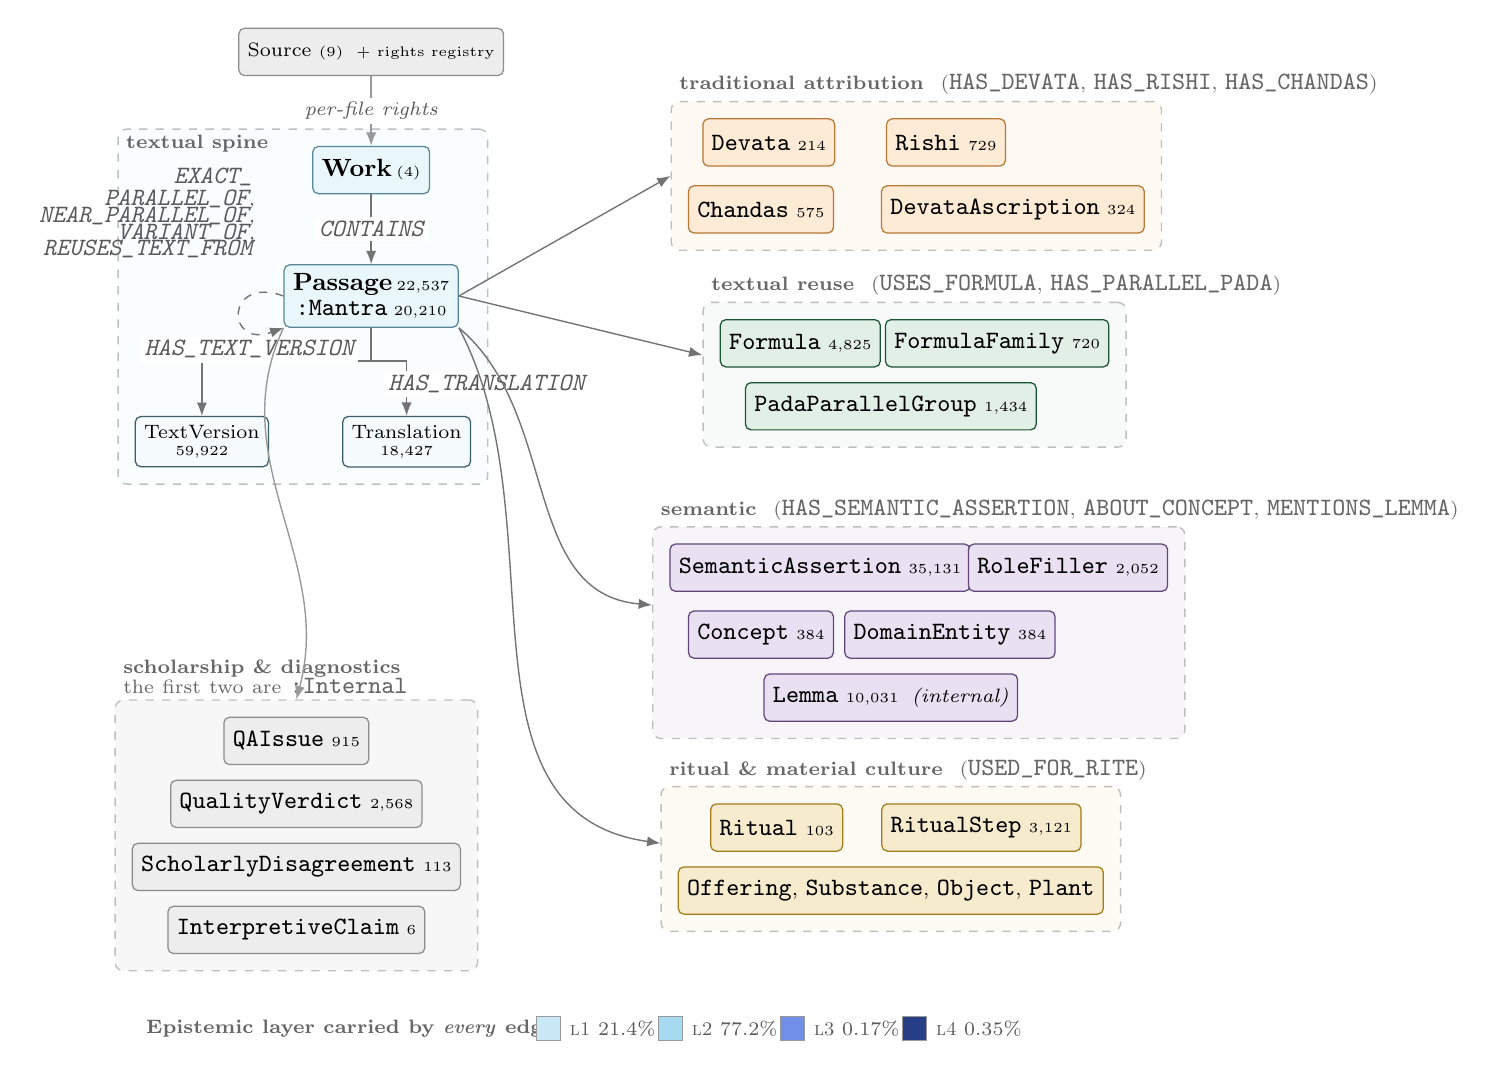
\begin{tikzpicture}[
  font=\footnotesize,
  every node/.style={align=center},
  ent/.style={draw=black!45, rounded corners=2pt, inner sep=3.2pt, fill=white,
              minimum height=6.0mm, line width=0.45pt, font=\scriptsize},
  spine/.style={ent, fill=SkyBlue!18, draw=SkyBlue!65!black, font=\small},
  sub/.style={ent, fill=SkyBlue!8, draw=SkyBlue!45!black},
  attr/.style={ent, fill=BurntOrange!14, draw=BurntOrange!70!black},
  sem/.style={ent, fill=RoyalPurple!11, draw=RoyalPurple!60!black},
  reuse/.style={ent, fill=SeaGreen!14, draw=SeaGreen!60!black},
  rit/.style={ent, fill=Goldenrod!22, draw=Goldenrod!75!black},
  meta/.style={ent, fill=black!7, draw=black!45},
  grp/.style={draw=black!25, rounded corners=3pt, inner sep=6pt, dashed,
              line width=0.5pt},
  ttl/.style={font=\scriptsize\bfseries, text=black!60, inner sep=1pt},
  rel/.style={-{Latex[length=1.7mm,width=1.3mm]}, draw=black!55, line width=0.5pt},
  lbl/.style={font=\scriptsize\itshape, inner sep=1.5pt, fill=white, text=black!65},
]

% ============ textual spine, centre-left column ============
\node[spine] (work) at (0,0)      {\textbf{Work}\,\tiny(4)};
\node[spine] (pass) at (0,-1.6)   {\textbf{Passage}\,\tiny 22{,}537\\[-2pt]
                                   \tiny\code{:Mantra} 20{,}210};
\node[sub]   (tv)   at (-2.15,-3.45) {TextVersion\\[-2pt]\tiny 59{,}922};
\node[sub]   (tr)   at ( 0.45,-3.45) {Translation\\[-2pt]\tiny 18{,}427};

\draw[rel] (work) -- node[lbl] {\code{CONTAINS}} (pass);
\draw[rel] (pass.south) -- ++(0,-0.42) -| (tv.north);
\draw[rel] (pass.south) -- ++(0,-0.42) -| (tr.north);
\node[lbl, anchor=east] at (-0.16,-2.28) {\code{HAS\_TEXT\_VERSION}};
\node[lbl, anchor=west] at ( 0.16,-2.72) {\code{HAS\_TRANSLATION}};

% self-loop for the four cross-textual predicates
\draw[rel, dashed] (pass.west) to[out=160,in=200,looseness=5] (pass.south west);
\node[lbl, anchor=east, text width=28mm, align=right, fill=none] at (-1.45,-0.55)
  {\code{EXACT\_PARALLEL\_OF},\\[-2pt]\code{NEAR\_PARALLEL\_OF},\\[-2pt]
   \code{VARIANT\_OF},\\[-2pt]\code{REUSES\_TEXT\_FROM}};

\node[meta] (src) at (0,1.5) {Source \tiny(9)\ \ $+$ rights registry};
\draw[rel, draw=black!40] (src) -- node[lbl] {\scriptsize per-file rights} (work);

\begin{scope}[on background layer]
  \node[grp, fill=SkyBlue!5, fit=(work)(pass)(tv)(tr)] (gspine) {};
\end{scope}
\node[ttl, anchor=north west] at ($(gspine.north west)+(2pt,-1pt)$) {textual spine};

% ============ attribution family, right, top ============
\node[attr] (dev) at (5.05,0.35)  {\code{Devata} \tiny 214};
\node[attr] (rsi) at (7.30,0.35)  {\code{Rishi} \tiny 729};
\node[attr] (chn) at (4.95,-0.50) {\code{Chandas} \tiny 575};
\node[attr] (asc) at (8.15,-0.50) {\code{DevataAscription} \tiny 324};
\begin{scope}[on background layer]
  \node[grp, fill=BurntOrange!4, fit=(dev)(rsi)(chn)(asc)] (gattr) {};
\end{scope}
\node[ttl, anchor=south west] at ($(gattr.north west)+(2pt,1pt)$)
  {traditional attribution\ \ \scriptsize\mdseries(\code{HAS\_DEVATA},
   \code{HAS\_RISHI}, \code{HAS\_CHANDAS})};

% ============ textual reuse family ============
\node[reuse] (form) at (5.45,-2.2) {\code{Formula} \tiny 4{,}825};
\node[reuse] (fam)  at (7.95,-2.2) {\code{FormulaFamily} \tiny 720};
\node[reuse] (ppg)  at (6.6,-3.0)  {\code{PadaParallelGroup} \tiny 1{,}434};
\begin{scope}[on background layer]
  \node[grp, fill=SeaGreen!4, fit=(form)(fam)(ppg)] (greuse) {};
\end{scope}
\node[ttl, anchor=south west] at ($(greuse.north west)+(2pt,1pt)$)
  {textual reuse\ \ \scriptsize\mdseries(\code{USES\_FORMULA},
   \code{HAS\_PARALLEL\_PADA})};

% ============ semantic family ============
\node[sem] (sa)   at (5.70,-5.05) {\code{SemanticAssertion} \tiny 35{,}131};
\node[sem] (conc) at (4.95,-5.90)  {\code{Concept} \tiny 384};
\node[sem] (de)   at (7.35,-5.90) {\code{DomainEntity} \tiny 384};
\node[sem] (rf)   at (8.85,-5.05) {\code{RoleFiller} \tiny 2{,}052};
\node[sem] (lem)  at (6.6,-6.70)  {\code{Lemma} \tiny 10{,}031
                                   \ \scriptsize\itshape(internal)};
\begin{scope}[on background layer]
  \node[grp, fill=RoyalPurple!4, fit=(sa)(conc)(de)(rf)(lem)] (gsem) {};
\end{scope}
\node[ttl, anchor=south west] at ($(gsem.north west)+(2pt,1pt)$)
  {semantic\ \ \scriptsize\mdseries(\code{HAS\_SEMANTIC\_ASSERTION},
   \code{ABOUT\_CONCEPT}, \code{MENTIONS\_LEMMA})};

% ============ ritual family ============
\node[rit] (rite) at (5.15,-8.35) {\code{Ritual} \tiny 103};
\node[rit] (step) at (7.75,-8.35) {\code{RitualStep} \tiny 3{,}121};
\node[rit] (offr) at (6.6,-9.15)  {\code{Offering}, \code{Substance},
                                   \code{Object}, \code{Plant}};
\begin{scope}[on background layer]
  \node[grp, fill=Goldenrod!5, fit=(rite)(step)(offr)] (grit) {};
\end{scope}
\node[ttl, anchor=south west] at ($(grit.north west)+(2pt,1pt)$)
  {ritual \& material culture\ \ \scriptsize\mdseries(\code{USED\_FOR\_RITE})};

% ============ diagnostics, bottom left ============
\node[meta] (qa)  at (-0.95,-7.25) {\code{QAIssue} \tiny 915};
\node[meta] (qv)  at (-0.95,-8.05) {\code{QualityVerdict} \tiny 2{,}568};
\node[meta] (sch) at (-0.95,-8.85) {\code{ScholarlyDisagreement} \tiny 113};
\node[meta] (ic)  at (-0.95,-9.65) {\code{InterpretiveClaim} \tiny 6};
\begin{scope}[on background layer]
  \node[grp, fill=black!3, fit=(qa)(qv)(sch)(ic)] (gmeta) {};
\end{scope}
\node[ttl, anchor=south west, text width=40mm, align=left]
  at ($(gmeta.north west)+(2pt,1pt)$)
  {scholarship \& diagnostics\\[-1pt]
   \scriptsize\mdseries the first two are \code{:Internal}};

% ============ spine-to-family edges ============
\draw[rel] (pass.east) -- ($(gattr.west)+(0,0)$);
\draw[rel] (pass.east) -- ($(greuse.west)+(0,0.25)$);
\draw[rel] (pass.south east) to[out=-40,in=175] ($(gsem.west)+(0,0.35)$);
\draw[rel] (pass.south east) to[out=-62,in=172] ($(grit.west)+(0,0.2)$);
\draw[rel, draw=black!40] (pass.south west) to[out=-115,in=75] (gmeta.north);

% ============ evidence-layer key ============
\begin{scope}[shift={(-2.9,-10.9)}]
  \node[ttl, anchor=west] at (0,0) {Epistemic layer carried by \emph{every} edge:};
  \foreach \i/\c/\t in {0/{SkyBlue!45}/{\textsc{l1} 21.4\%},
                        1/{SkyBlue!75}/{\textsc{l2} 77.2\%},
                        2/{RoyalBlue!75}/{\textsc{l3} 0.17\%},
                        3/{RoyalBlue!60!black}/{\textsc{l4} 0.35\%}} {
    \node[draw=black!40, fill=\c, minimum width=3mm, minimum height=3mm,
          inner sep=0pt, line width=0.4pt] at ({5.15+\i*1.55},0) {};
    \node[font=\scriptsize, text=black!65, anchor=west]
      at ({5.3+\i*1.55},0) {\t};
  }
\end{scope}
\end{tikzpicture}
}
\caption{Core graph ontology, grouped by object family. An overview: 55 node labels
and 81 relationship types are in use, and the full catalogue is
\cref{sec:appendix-ontology}. The figure shows one labelled edge per family rather
than every predicate, because the alternative is unreadable. Counts are from the
fact freeze at \code{6bf220c}.}
\label{fig:ontology}
\end{figure}

\subsection{Four axes, deliberately not collapsed}

The object families are shown in \cref{fig:ontology}. Every relationship in
VedGraph carries, as stored properties, the answers to four different questions. They are orthogonal, and the model's central claim is that
collapsing any pair makes a well-formed scholarly question unaskable.

\paragraph{(1) How did this claim come to be?} The \emph{knowledge layer} is a
four-member closed vocabulary, described in the code as ``never collapsed, never
inferred from a score'':

% generated by figures-src/make_tables.py -- do not edit
\begin{table}[tb]
\centering
\caption{Relationships by epistemic layer, measured on the live graph at
\code{6bf220c}. The layer is a stored, indexed edge property, so this distribution is
a query rather than an estimate. Two pipeline generations wrote the field with and
without the \code{L}-prefix; the legacy spellings are folded here and reported
unfolded in the fact freeze.}
\label{tab:layers}
\small
\begin{tabularx}{\linewidth}{@{}l>{\raggedright\arraybackslash}Xrr@{}}
\toprule
Layer & Meaning & Edges & \% \\
\midrule
\Lone & \footnotesize a source states it & 109{,}298 & 21.39 \\
\Ltwo & \footnotesize a reproducible rule over stored text or over \vocab{l1} & 394{,}540 & 77.22 \\
\Lthree & \footnotesize a language model read evidence and proposed it & 890 & 0.17 \\
\Lfour & \footnotesize a reading held by this project or a named commentator & 1{,}787 & 0.35 \\
untyped (a recorded defect) & \footnotesize no layer recorded; see \cref{sec:threats} & 4{,}390 & 0.86 \\
\midrule
\textbf{Total} & & \textbf{510{,}905}
& \textbf{100.00} \\
\bottomrule
\end{tabularx}
\end{table}


\paragraph{(2) How should a reader grade it?} The \emph{quality tier} is a
reader-facing letter derived from the layer by a total bijection
($\textsc{l1}\!\to\!\textsc{a}$, $\textsc{l2}\!\to\!\textsc{b}$,
$\textsc{l3}\!\to\!\textsc{c}$, $\textsc{l4}\!\to\!\textsc{d}$). The module states the
rule as: tier is how a claim was reached, never how confident it sounds. The tier
exists separately from the layer because one further transition acts on it --- a
model-extracted claim that no reviewer has accepted stays in \textsc{l3} but drops to
\textsc{tier\,d}, since \textsc{tier\,c} is defined as model-extracted evidence that
survived review and a candidate has not had any.

\paragraph{(3) What is the claim's reach over the passage?} \emph{Attribution
precision} distinguishes a per-passage statement, a label \emph{inherited} from an
enclosing container, the passage's own wording, and edges that are not attributions at
all. This is the axis that matters most for counting. The Anukrama\d{n}\=\i\ names a
deity for a \iast{s\=ukta}; projecting that label onto each of its mantras is what
makes ``passages of Indra'' work at all, but a reader who cannot see the difference
reads tens of thousands of inherited labels as per-verse statements. The model records
the consequence: ``How many mantras invoke Indra?'' has at least four honest answers
--- strict source-stated, container-inherited, textual mention, and semantic
invocation --- and collapsing any pair of them makes one of the four unaskable. The
live distribution shows how unevenly the corpus behaves: every one of the
V\=ajasaneyi Sa\d{m}hit\=a's 2{,}240 seer attributions is source-stated per verse,
while every one of the Atharvaveda's 5{,}084 is a \iast{s\=ukta} label projected
downward, so a per-verse Atharvavedic seer claim cannot be made from this corpus at
all.

\paragraph{(4) Off which textual surface was the evidence read?} A rule fired over
Griffith's 1896 English is exactly as reproducible as a rule fired over the Sanskrit,
so the tier cannot separate them --- and the difference matters enormously, because
one measures a Victorian translator's word choice and the other measures the text.
The project discovered this the expensive way: 21{,}246 of 47{,}542
\code{ABOUT\_CONCEPT} edges had fired on an English keyword with no Sanskrit evidence
and carried an identical grade to edges matched on the verse itself. Those edges were
later withdrawn, and a separate \emph{evidence surface} axis was introduced so the
distinction is filterable rather than archaeological.

\subsection{A name collision, and what it cost}
\label{sec:collision}

The fourth axis is instructive as a failure. Two different enumerations in the
codebase are both called \code{EvidenceBasis}. One describes the textual surface the
evidence was read off; the other describes the kind of act that produced the claim.
Their value spaces are disjoint. Reading the stored graph property straight into the
second enumeration --- the natural thing to do, given the shared name --- mapped
\emph{every} attribution edge in the corpus to \code{UNKNOWN}: all 17{,}889 seer
edges, all 16{,}298 metre edges, all 10{,}558 deity edges. The failure was silent,
because \code{UNKNOWN} is a legitimate value.

The remedy is worth reporting because it generalises. Rather than renaming one
enumeration, the project added a test that enumerates the property's entire observed
value space in the live store and asserts it is a subset of the surface vocabulary.
The test's header records why the check is shaped that way: this project has twice
certified an absence by asking the wrong question, once against the wrong surface and
once with the wrong vocabulary. Grepping for the value you expect confirms your
expectation; enumerating the value space does not.

\subsection{The lifecycle: a model may write exactly one status}
\label{sec:model-policy}

The constraint that keeps \textsc{l3} small is not a review convention. It is encoded
as data. Assertion state is a three-member vocabulary --- candidate, accepted,
rejected --- and the set of trust classes permitted to be written as \emph{accepted}
without review is a frozen set containing exactly deterministic-derived and
source-explicit. The comment beside it is explicit that this is the policy expressed
as data rather than as a convention. The constructor raises if a model-derived record
is marked accepted, and raises again if a record claims model provenance without
naming a model.

The governing decision record, \mbox{ADR-014}, states the rule and three consequences
that are each enforced in code:

\begin{quote}\small
A model may write exactly one status: \code{CANDIDATE}. Every other status is written
by a deterministic stage or by a person. \dots{} Evidence is checkable or the claim is
discarded: a cited token the model was never shown is a fabricated citation, it is
decidable, and it is rejected. \dots{} The predicate vocabulary is closed, and the
refusals are named. \dots{} Confidence is a floor inside a predicate's rule and
nothing else: acceptance requires that the predicate has been \emph{unlocked} by a
measured gold precision of $\ge 95\,\%$; until then, a confidence of 1.0 is accepted at
the same rate as 0.4 --- not at all.
\end{quote}

Its stated rationale is the reason we treat confidence-thresholding as unsound in this
setting: the confidence score is produced by the same process that produced the claim,
so it carries no information independent of the claim, and thresholding on it selects
for fluency rather than for truth. The unlocked-predicate set is empty by
construction and remains empty; consequently no semantic assertion has ever been
auto-accepted.

Two refinements are worth noting. First, five predicates that a model might naturally
want --- \code{SYMBOLIZES}, \code{REPRESENTS}, \code{IS\_GOD\_OF}, \code{MEANS},
\code{CAUSES} --- are members of the enumeration \emph{so that a proposal naming one
is rejected as a policy decision with a recorded reason}, rather than failing schema
validation as an unknown string. The difference matters when reading a rejection
report. Second, the strongest review state the graph has ever recorded is
\code{MODEL\_ADJUDICATED}, glossed in the API as ``a model re-read the passage and
accepted this edge with a stated reason. This is the strongest review state in this
graph and it is not human review.'' The count of human-reviewed edges is zero, and the
product says so.

\begin{figure}[tbp]
\centering
\resizebox{0.93\textwidth}{!}{% Figure: the epistemic pipeline -- how a claim acquires, and keeps, its typing.
% Centre column: the state the claim is in. Left: who acts. Right: what travels with
% the claim. Bottom: the four terminal dispositions, reached by dedicated routing
% channels either side of the centre column so no connector crosses annotation text.
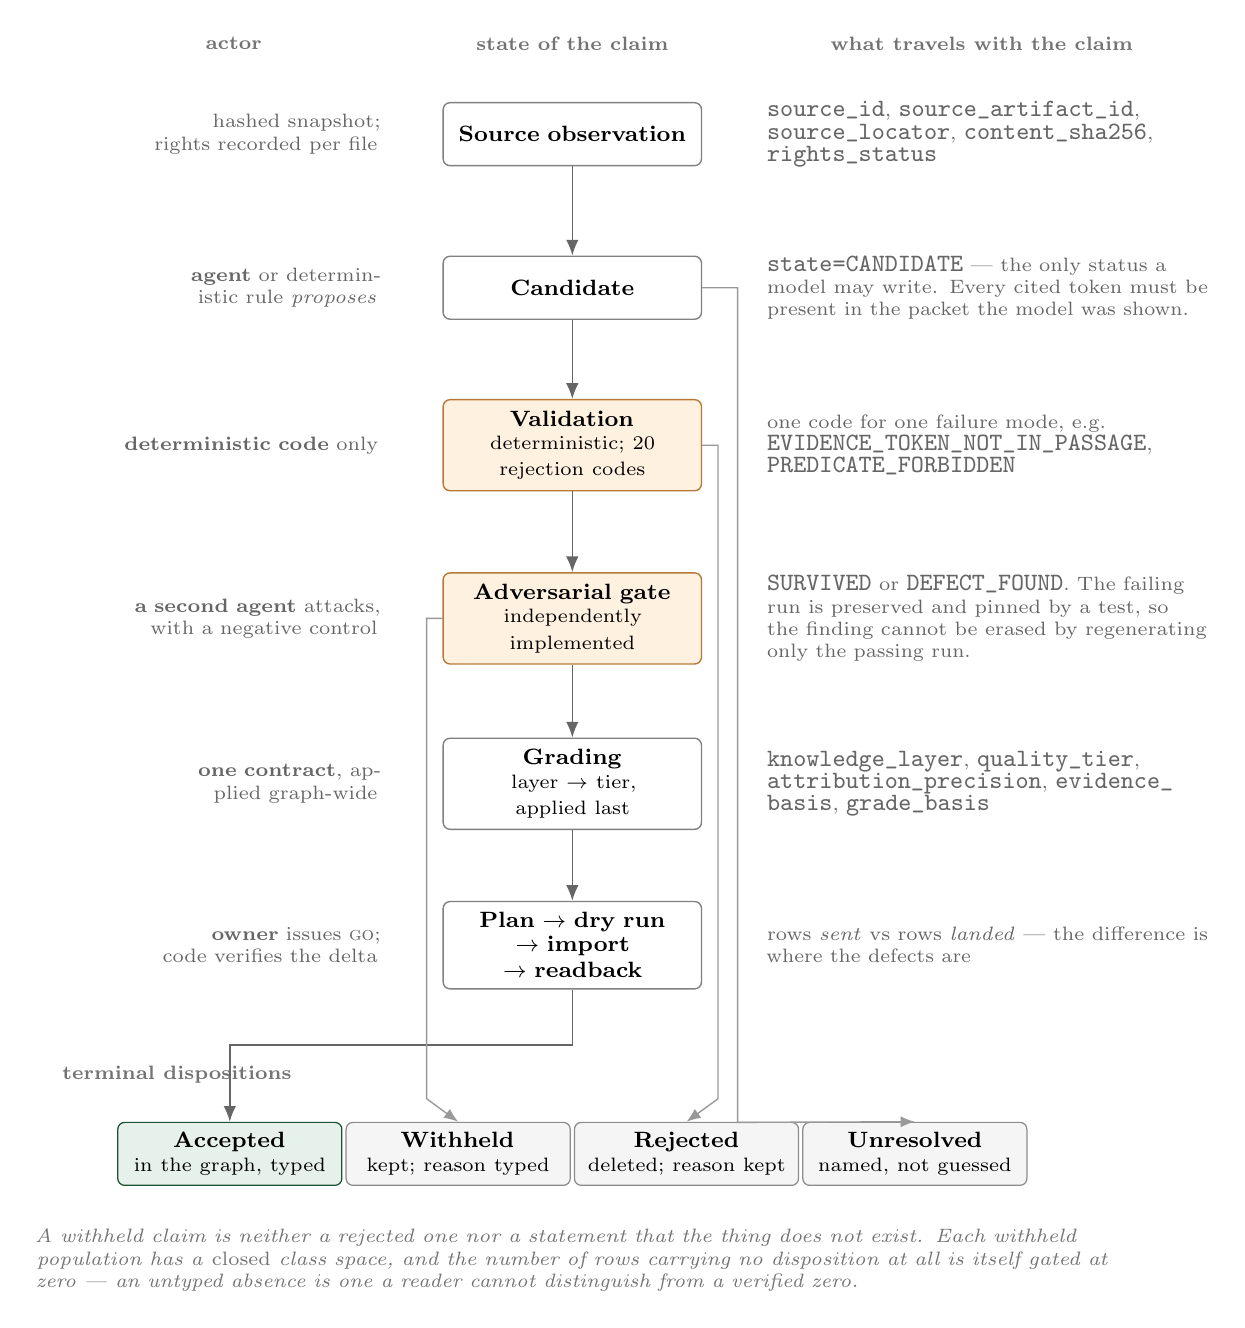
\begin{tikzpicture}[
  font=\footnotesize,
  every node/.style={align=center},
  st/.style={draw=black!50, rounded corners=2.5pt, inner sep=4pt, fill=white,
             minimum width=30mm, text width=30mm, minimum height=8mm,
             line width=0.5pt},
  gate/.style={st, draw=BurntOrange!70!black, fill=BurntOrange!10},
  term/.style={draw=black!45, rounded corners=2.5pt, inner sep=3.5pt, fill=black!4,
               minimum width=26mm, text width=26mm, minimum height=8mm,
               line width=0.45pt},
  acc/.style={term, fill=SeaGreen!12, draw=SeaGreen!60!black},
  flow/.style={-{Latex[length=2mm,width=1.6mm]}, draw=black!60, line width=0.6pt},
  route/.style={-{Latex[length=1.8mm,width=1.4mm]}, draw=black!40, line width=0.5pt},
  lft/.style={font=\scriptsize, text=black!60, align=right, text width=40mm,
              anchor=east},
  rgt/.style={font=\scriptsize, text=black!60, align=left, text width=56mm,
              anchor=west},
  hd/.style={font=\scriptsize\bfseries, text=black!55},
]

\def\L{-2.35}   % right edge of the left annotation column
\def\R{2.35}    % left edge of the right annotation column

\node[hd] at (-4.3,1.15) {actor};
\node[hd] at (0,1.15)    {state of the claim};
\node[hd] at (5.2,1.15)  {what travels with the claim};

\node[st]  (src)  at (0,0)     {\textbf{Source observation}};
\node[st]  (cand) at (0,-1.95) {\textbf{Candidate}};
\node[gate](val)  at (0,-3.95) {\textbf{Validation}\\[-1pt]
                                \scriptsize deterministic; 20 rejection codes};
\node[gate](adv)  at (0,-6.15) {\textbf{Adversarial gate}\\[-1pt]
                                \scriptsize independently implemented};
\node[st]  (grade)at (0,-8.25) {\textbf{Grading}\\[-1pt]
                                \scriptsize layer $\to$ tier, applied last};
\node[st]  (imp)  at (0,-10.3) {\textbf{Plan $\to$ dry run}\\[-1pt]
                                \textbf{$\to$ import $\to$ readback}};

\foreach \a/\b in {src/cand, cand/val, val/adv, adv/grade, grade/imp}
  \draw[flow] (\a) -- (\b);

% ---- left column: actors ----
\node[lft] at (\L,0)      {hashed snapshot; rights recorded per file};
\node[lft] at (\L,-1.95)  {\textbf{agent} or deterministic rule \emph{proposes}};
\node[lft] at (\L,-3.95)  {\textbf{deterministic code} only};
\node[lft] at (\L,-6.15)  {\textbf{a second agent} attacks, with a negative control};
\node[lft] at (\L,-8.25)  {\textbf{one contract}, applied graph-wide};
\node[lft] at (\L,-10.3)  {\textbf{owner} issues \textsc{go}; code verifies the delta};

% ---- right column: what travels ----
\node[rgt] at (\R,0)     {\code{source\_id}, \code{source\_artifact\_id},
                          \code{source\_locator}, \code{content\_sha256},
                          \code{rights\_status}};
\node[rgt] at (\R,-1.95) {\code{state=CANDIDATE} --- the only status a model may
                          write. Every cited token must be present in the packet the
                          model was shown.};
\node[rgt] at (\R,-3.95) {one code for one failure mode, e.g.\
                          \code{EVIDENCE\_TOKEN\_NOT\_IN\_PASSAGE},
                          \code{PREDICATE\_FORBIDDEN}};
\node[rgt] at (\R,-6.15) {\code{SURVIVED} or \code{DEFECT\_FOUND}. The failing run is
                          preserved and pinned by a test, so the finding cannot be
                          erased by regenerating only the passing run.};
\node[rgt] at (\R,-8.25) {\code{knowledge\_layer}, \code{quality\_tier},
                          \code{attribution\_precision}, \code{evidence\_basis},
                          \code{grade\_basis}};
\node[rgt] at (\R,-10.3) {rows \emph{sent} vs rows \emph{landed} --- the difference is
                          where the defects are};

% ---- terminal dispositions ----
\def\TY{-12.95}
\node[acc]  (t1) at (-4.35,\TY) {\textbf{Accepted}\\[-1pt]
                                 \scriptsize in the graph, typed};
\node[term] (t2) at (-1.45,\TY) {\textbf{Withheld}\\[-1pt]
                                 \scriptsize kept; reason typed};
\node[term] (t3) at ( 1.45,\TY) {\textbf{Rejected}\\[-1pt]
                                 \scriptsize deleted; reason kept};
\node[term] (t4) at ( 4.35,\TY) {\textbf{Unresolved}\\[-1pt]
                                 \scriptsize named, not guessed};
\node[hd, anchor=west] at (-6.6,-11.95) {terminal dispositions};

% routing channels: x=-1.85 / -2.1 on the left, x=1.85 / 2.1 on the right.
% The annotation columns start at +/-2.35, so nothing crosses text.
\draw[flow] (imp.south) -- ++(0,-0.7) -| (t1.north);
\draw[route] (adv.west)  -- (-1.85,-6.15) -- (-1.85,-12.25) -- (t2.north);
\draw[route] (val.east)  -- ( 1.85,-3.95) -- ( 1.85,-12.25) -- (t3.north);
\draw[route] (cand.east) -- ( 2.10,-1.95) -- ( 2.10,-12.55) -- (t4.north);

\node[font=\scriptsize\itshape, text=black!55, text width=13.6cm, align=left]
  at (0,-14.3)
  {A withheld claim is neither a rejected one nor a statement that the thing does not
   exist. Each withheld population has a \emph{closed} class space, and the number of
   rows carrying no disposition at all is itself gated at zero --- an untyped absence
   is one a reader cannot distinguish from a verified zero.};
\end{tikzpicture}
}
\caption{The epistemic pipeline: how a claim acquires its typing and what it can
terminally become. The centre column is the state of the claim, the left gutter names
the actor, and the right gutter names what travels with the claim at that point.
Only one of the four terminal dispositions puts a claim in the graph; the other three
are recorded rather than discarded, because an absence a reader cannot distinguish
from a verified zero is the most misleading thing this graph could publish.}
\label{fig:epistemic}
\end{figure}

\subsection{Typed absence}
\label{sec:typed-absence}

\Cref{fig:epistemic} sets out the whole lifecycle, from a source observation to one
of four terminal dispositions. The model treats an untyped absence as a defect. Four distinct mechanisms record
\emph{why} something is not present, each scoped to a layer: a reason string per
unmapped predicate, emitted into the load report alongside a separate count of
predicates that are neither mapped nor explicitly withheld (``not mapped'' and
``nobody looked'' are indistinguishable in a coverage number, and only one of them is
acceptable); a typed node property with a declared, closed class space, used for
S\=amavedic notation (\cref{sec:case-samaveda}); typed non-resolution rows in the
lexical layer, where 711 unresolved tokens each carry a linguistic reason rather than
a queue state; and edge-type-keyed withholding, where near-parallel pairs are held
back from a reuse claim with the reason recorded on the type.

The invariant that makes the S\=amavedic case work is published as a measurement
rather than asserted: the count of verses with no notation disposition at all must be
zero, because an untyped verse is one a reader cannot tell apart from a verified zero.

\subsection{The public boundary, and a label that does two jobs}

Product and internal knowledge share one database. Diagnostic nodes --- the
repository's assessments of its own passages --- carry a marker label so that a single
filter, written once, excludes them. The design note is that sprinkling an exclusion
across thirty queries would be the same policy enforced thirty times and wrong the
first time a new diagnostic label appeared.

The marker turns out to mark two different kinds of node, and the distinction is not
drawn by the label itself. It marks the diagnostic layer, which no researcher should
traverse into, and it marks \emph{sub-entities} --- text versions, translations,
lemmas, sources --- which must stay reachable, since a passage that could not reach
its own text would be useless. The broad form of the obvious leakage check therefore
reports 70{,}559 ``leaks'', every one of them legitimate, and an auditor running it
would file a false critical finding. The invariant is consequently written against the
diagnostic labels by name rather than against the marker.

A related caveat is structural and is worth stating for anyone building on such a
graph: the separation is query-side, not structural. An unfiltered one-hop traversal
from any passage returns tens of thousands of text-version and translation nodes. The
mitigation the project adopts is to serve a catalogue of vetted queries rather than
the database.

\subsection{Invariants}
\label{sec:invariants}

Twenty live invariants and twelve integrity gates run against the loaded store. The
design principle is stated in the invariant suite's header: each check is phrased as
the defect it detects rather than as the desired state, because each corresponds to a
defect this repository actually shipped. Representative members include: no edge
without a quality tier; no edge without a grade rationale; no unlabelled node; no
product node reaching a diagnostic node; no work without a scope statement; no
attribution-precision value outside the declared enumeration; no predicate carrying
more than one run identifier, since that would mean part of the graph is reproducible
from no committed artefact.

Two features of this suite bear on method. First, one gate had been rewritten twice
and both earlier versions were untestable --- they computed the set of declared
relationship types as the union of the ontology \emph{and the graph}, then asked which
graph types were missing from it. Nothing can be. The gate reported zero undeclared
types for an entire wave while eleven predicates went unclassified. The code now
carries the lesson as a comment: the data may not declare itself valid. Second, a
universal-quantifier invariant over attribution precision could only be written safely
once the vocabulary had a member meaning ``this edge is not an attribution'' ---
an invariant asserting that every edge carries a property must first be able to say
what the property means on every edge.

\section{Agentic Construction}
\label{sec:agentic}

\subsection{What ``agentic'' means here, and what it does not}

The construction ran in a coding-agent runtime: a language model with filesystem,
shell and database access, directed by one human owner, writing and executing code as
well as reading sources. It did \emph{not} use ReAct, AutoGen, LangGraph, CrewAI,
Reflexion or any comparable orchestration library; we searched the project's
dependency manifests and found none, and we mention the families only because the
related-work section discusses them (\cref{sec:related}). Orchestration here is the
project's own artefact protocol --- briefs, staging directories, proposal files,
gates, rulings and receipts --- rather than a framework.

Two consequences follow. The workflow is inspectable, because each step left a file.
And it is not a reusable system: what generalises is the protocol, not an
implementation.

\begin{figure}[tbp]
\centering
\resizebox{0.86\textwidth}{!}{% Figure: the construction pipeline, with the actor for each stage in the left
% gutter and what the stage may not do in the right gutter. Reconstructed from the
% repository's own artefact protocol; every stage names a file family that exists.
\begin{tikzpicture}[
  font=\footnotesize,
  every node/.style={align=center},
  st/.style={draw=black!50, rounded corners=2.5pt, inner sep=4.5pt, fill=white,
             text width=44mm, minimum height=7mm, line width=0.55pt},
  det/.style={st, fill=SeaGreen!10, draw=SeaGreen!60!black},
  agn/.style={st, fill=SkyBlue!14, draw=SkyBlue!65!black},
  adv/.style={st, fill=BurntOrange!11, draw=BurntOrange!70!black},
  own/.style={st, fill=RoyalPurple!9, draw=RoyalPurple!60!black},
  fin/.style={st, fill=black!6, draw=black!60, line width=0.8pt},
  fl/.style={-{Latex[length=2.1mm,width=1.6mm]}, draw=black!60, line width=0.7pt},
  who/.style={font=\scriptsize\bfseries, text=black!58, anchor=east,
              text width=26mm, align=right},
  nope/.style={font=\scriptsize, text=black!58, anchor=west, text width=52mm,
               align=left},
  hd/.style={font=\scriptsize\bfseries, text=black!52},
]

\node[hd] at (-5.1,1.15) {actor};
\node[hd] at (0,1.15) {stage};
\node[hd] at (5.3,1.15) {what the stage may not do};

\node[det] (s1) at (0,0.25)   {\textbf{Source acquisition}\\[-1pt]
                               \tiny hashed snapshot; rights recorded per file};
\node[det] (s2) at (0,-1.45)  {\textbf{Canonical corpus + identity}\\[-1pt]
                               \tiny \mbox{UUIDv5} over a \mbox{URN};
                               byte-reproducible build};
\node[agn] (s3) at (0,-3.55)  {\textbf{Parallel layer proposal}\\[-1pt]
                               \tiny one staging directory per domain\\[2pt]
                               \tiny\itshape attribution \textperiodcentered\ textual
                               reuse \textperiodcentered\ formulae
                               \textperiodcentered\ entities
                               \textperiodcentered\ ritual\\[-1pt]
                               \tiny\itshape translation \textperiodcentered\ notation
                               \textperiodcentered\ audio\\[2pt]
                               \tiny eight layers, proposed independently;\\[-1pt]
                               \tiny each lands in staging, none in the graph};
\node[det] (s4) at (0,-5.35)  {\textbf{Staging validation}\\[-1pt]
                               \tiny the contract reports its own coverage};
\node[adv] (s5) at (0,-7.05)  {\textbf{Gates A / B / C}\\[-1pt]
                               \tiny integrity, conformance, attack};
\node[det] (s6) at (0,-8.75)  {\textbf{Grading}\\[-1pt]
                               \tiny layer, tier, precision, surface ---
                               applied graph-wide, last};
\node[own] (s7) at (0,-10.55) {\textbf{Plan $\to$ dry run $\to$ \textsc{go}
                               $\to$ import $\to$ readback}};
\node[det] (s8) at (0,-12.45) {\textbf{Invariants and scorecard}\\[-1pt]
                               \tiny 20 invariants, 11 gates, all at zero};
\node[fin] (s9) at (0,-14.15) {\textbf{VedGraph}\\[-1pt]
                               \tiny 165{,}737 nodes, 510{,}905 relationships};
\node[fin] (s10) at (0,-15.65){\textbf{VedAnvaya}\\[-1pt]
                               \tiny read-only \mbox{API} and interface};

\foreach \a/\b in {s1/s2, s2/s3, s3/s4, s4/s5, s5/s6, s6/s7, s7/s8, s8/s9, s9/s10}
  \draw[fl] (\a) -- (\b);


% ---- left gutter: actor ----
\node[who] at (-2.45,0.25)    {deterministic};
\node[who] at (-2.45,-1.45)   {deterministic};
\node[who] at (-2.45,-3.35)   {\textbf{agent}\\proposes};
\node[who] at (-2.45,-5.35)   {deterministic};
\node[who] at (-2.45,-7.05)   {\textbf{a second agent}\\attacks};
\node[who] at (-2.45,-8.75)   {deterministic};
\node[who] at (-2.45,-10.55)  {\textbf{owner} \textsc{go};\\code verifies};
\node[who] at (-2.45,-12.45)  {deterministic};
\node[who] at (-2.45,-14.15)  {---};
\node[who] at (-2.45,-15.65)  {---};

% ---- right gutter: the refusal at each stage ----
\node[nope] at (2.45,0.25)
  {a permissive licence is never inferred, only evidenced; absence of a licence
   field is not a grant};
\node[nope] at (2.45,-1.45)
  {no source, text, script, edition, build or sequence position may enter an
   identifier};
\node[nope] at (2.45,-3.35)
  {a model may write exactly one status, \code{CANDIDATE}; the predicate
   vocabulary is closed and its refusals are named};
\node[nope] at (2.45,-5.35)
  {a check that skipped its population must show as a coverage shortfall, not as
   a pass};
\node[nope] at (2.45,-7.05)
  {Gate~C is a separate file from Gate~B, ``so the same codepath cannot validate
   itself'', and carries a negative control};
\node[nope] at (2.45,-8.75)
  {an unlisted relationship type \emph{raises}; the fall-through default is the
   weakest tier, never the strongest};
\node[nope] at (2.45,-10.55)
  {nothing is imported until a readback; an importer's own success report is not
   evidence};
\node[nope] at (2.45,-12.45)
  {the data may not declare itself valid --- a gate whose declared set includes
   the graph cannot fail};
\node[nope] at (2.45,-14.15)
  {every edge carries its epistemic layer, so a consumer can exclude
   model-derived claims with a predicate};
\node[nope] at (2.45,-15.65)
  {typing is rendered where the reader is, not on a methods page};

\end{tikzpicture}
}
\caption{The construction pipeline. The left gutter names the actor for each stage;
the right gutter names what that stage is forbidden to do, which is where the
method actually lives. Agents propose into staging; deterministic code validates,
grades and verifies; the owner issues the one decision that lets a mutation run.}
\label{fig:pipeline}
\end{figure}

\subsection{The construction pipeline}

\Cref{fig:pipeline} shows the pipeline the artefacts describe. Its spine is the same
for every layer: a source is snapshotted and hashed; a canonical corpus is built
deterministically and given identity; a layer is proposed into a \emph{staging}
directory that is validated and gated before any graph write; the owner issues a
\textsc{go} against a hashed plan; the import executes; and a readback compares what
was sent with what landed.

The staging step is the load-bearing one. A layer's proposal is a directory of
row-level JSONL plus a manifest, validated by a contract that reports \emph{its own
coverage} --- the validator states how many rows each check evaluated, so a check
that silently skipped its population is visible as a coverage shortfall rather than
as a pass. During the completeness campaign the rule was stated flatly: nothing is
imported until a readback.

\subsection{The import protocol}
\label{sec:import}

Every graph mutation in the later campaigns followed a five-step protocol, and its
steps exist because each was once skipped:

\begin{enumerate}[leftmargin=1.9em,itemsep=1pt,topsep=2pt]
\item \textbf{Plan.} A hashed artefact enumerating the exact nodes, edges and
property writes, with the expected census delta.
\item \textbf{Dry run.} The plan re-computed against the live graph, emitting a
\textsc{go} or the reason it cannot. Dry runs were regenerated whenever the tree
changed, because a dry run computed against a different state is not a dry run.
\item \textbf{Owner \textsc{go}.} A recorded human decision against a specific plan
hash.
\item \textbf{Execute.}
\item \textbf{Readback.} An independent re-measurement comparing rows \emph{sent}
against rows \emph{landed}, with the census delta checked against the promise.
\end{enumerate}

The protocol's value is measurable in what it caught: a first import that
over-wrote by 5{,}930 edges, a second that left 12{,}033 nodes unreachable, a third
that landed 13{,}187 elements the domain rules excluded, and one that silently
overwrote 102 curated display labels. Roughly nine plan/dry-run/\textsc{go} cycles
preceded one clean readback in the largest wave.

It also failed in an instructive way. One readback printed \code{READBACK\_CLEAN}
having compared zero rows against zero rows, and a separate import's own readback
reported success while two graph-wide contracts were unmet --- the scorecard, not the
importer, found 1{,}136 edges that were ungraded, unlabelled and unmarked. The
lesson the repository records is the one we would generalise: \emph{an importer's own
success report is not evidence}.

\subsection{The multi-agent structure, as the artefacts show it}
\label{sec:multiagent}

The clearest instance is the final closure sprint, and we describe it using the
repository's own names rather than inventing roles.

Forty-three remaining gaps were partitioned across \textbf{seven domain agents}, one
owner each, under a stated rule: every implementation-fixable row has exactly one
owner agent, and no row is unassigned. The agents are named by domain ---
\code{AGENT\_1\_FORMULA\_CROSS\_VEDA} (3 gaps),
\code{AGENT\_2\_ENTITY\_DEVATA\_IDENTITY} (12),
\code{AGENT\_3\_MORPHOLOGY\_SEMANTICS} (7), \code{AGENT\_4\_RITUAL} (4),
\code{AGENT\_5\_QUALITY\_REFERENCE} (6), \code{AGENT\_6\_PRODUCT\_SURFACE} (5) and
\code{AGENT\_7\_TRANSLATION\_SAMAVEDA} (6). Each produced measurements, row-level
evidence and a file named \code{proposed\_mutations.json}. \emph{None of them wrote
to the graph.}

An eighth agent had no gaps assigned. Its artefacts are an audit of the other seven,
its recorded database access is \code{READ\_ONLY}, and it is the adversary in the
pattern. A \textbf{lead} then reconciled proposals and findings into an integration
plan, a set of rulings and a receipt.

\Cref{fig:adversarial} shows the resulting cycle. Its most important property is
visible in one ruling. Agent~3 proposed re-anchoring a relationship so that role
fillers hang from semantic assertions. Agent~8 measured that the change would create
2{,}052 endpoint-signature violations, because the declared signature expects a
passage endpoint and zero of the assertion nodes carry that label. The lead verified
the measurement independently, and then ruled neither ``approved'' nor ``rejected''
but \emph{approved with the ontology moving in the same change} --- because the
migration card had declared the new signature all along, and either half alone would
leave 2{,}052 violations. A test now pins the signature to the card.

Three features of that ruling recur across the corpus of rulings and are, we think,
the transferable part:

\begin{itemize}[leftmargin=1.9em,itemsep=1pt,topsep=2pt]
\item \textbf{The adversary measures rather than opines.} Agent~8's findings are
counts against the live store, so they can be re-run. One of them --- that a
registry-status check ``only compared a graph measurement to a pre-declared integer;
it never read the status field'' --- is a defect in a \emph{check}, not in data.
\item \textbf{The integrator re-measures before ruling.} The lead's rulings record
\code{lead\_measurement} separately from the agent's claim, and in one case correct
the agent's figure: an agent measured the live layer at 4{,}865 unreviewed
assertions while its own staged delta would take the post-integration value to
35{,}139 --- a prediction, against the 35{,}131 the layer holds today.
\item \textbf{Trades are recorded, not netted.} One ruling notes that closing a
coverage gap multiplies another gap's unreviewed population sevenfold and deepens a
third, and records the trade instead of reporting the improvement alone.
\end{itemize}

The adversary also found defects nobody had a gap for. It measured that the exported
public artefact under-declared its own inputs --- 31 of 36 exported labels
undeclared, 129{,}691 edges and 32{,}044 node rows invisible to the hash that was
supposed to cover them, and 4{,}016 public nodes dropped silently. And it found a
user-visible search defect by querying rather than by reading code: 5{,}123 of 5{,}839
search derivatives in one corpus carried a private-use sentinel character, so a
reader searching for \iast{\d{r}tasya} got zero hits while the sentinel form got 94.

\begin{figure}[tbp]
\centering
\resizebox{\textwidth}{!}{% Figure: propose -> attack -> adjudicate, as the final closure sprint's artefacts
% record it. Names and counts are the repository's own (gap_assignment.json,
% agent8/audit_findings.json, lead/rulings.json); no role is invented to make the
% diagram symmetrical.
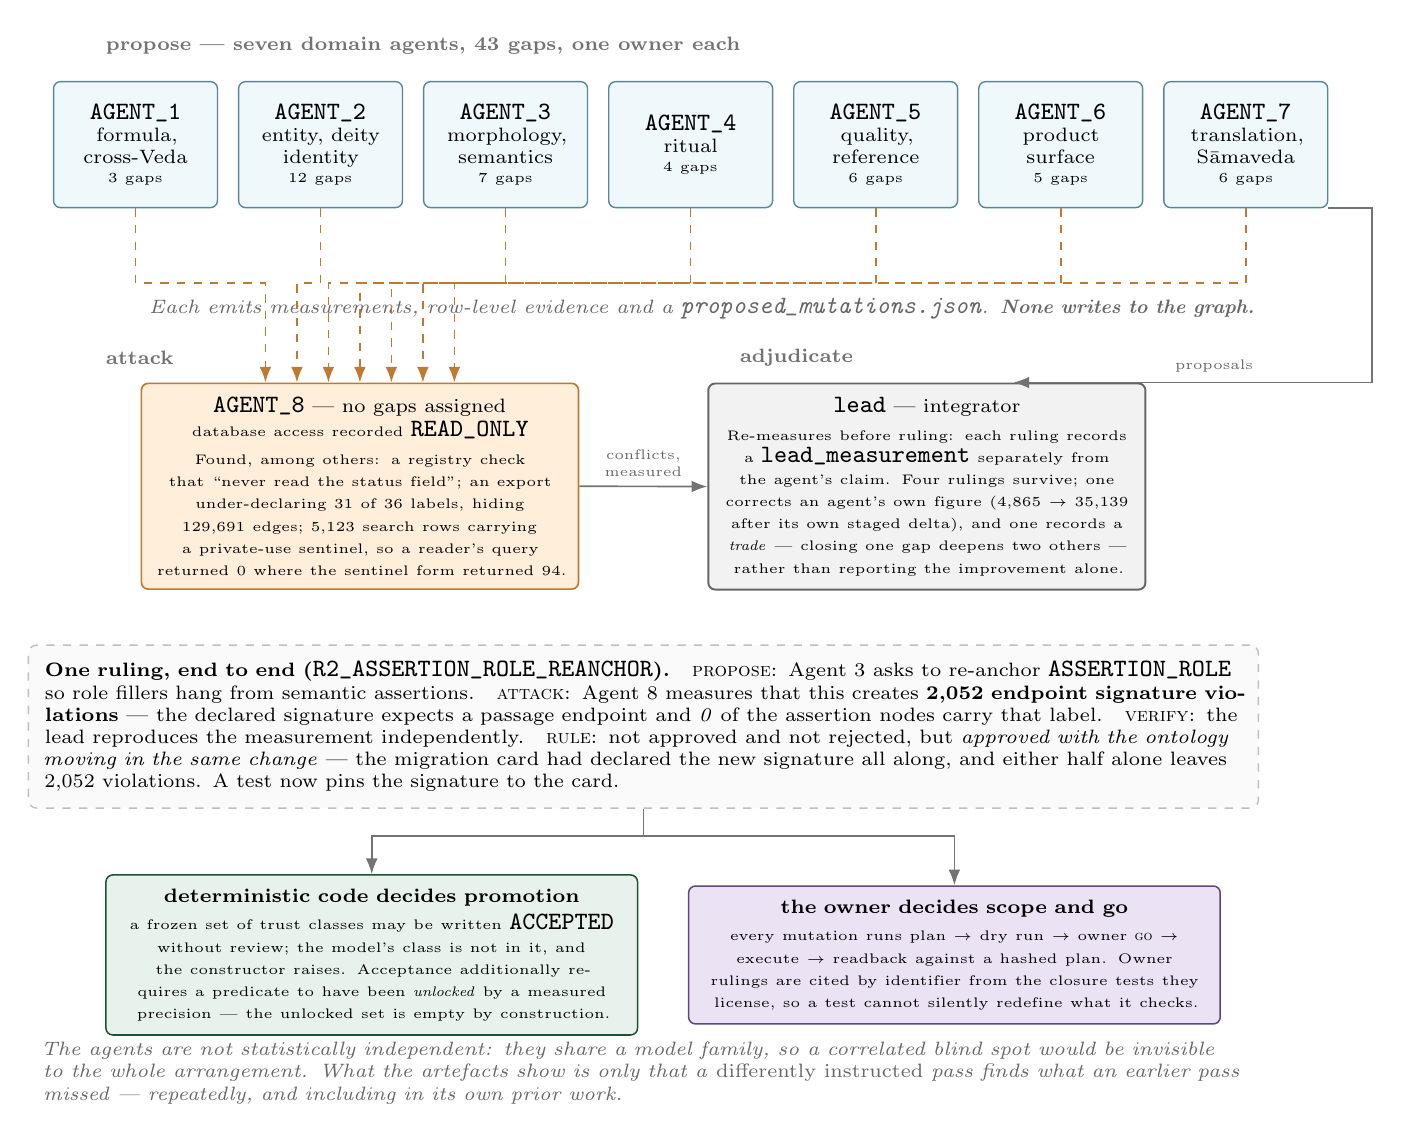
\begin{tikzpicture}[
  font=\footnotesize,
  every node/.style={align=center},
  ag/.style={draw=SkyBlue!65!black, fill=SkyBlue!13, rounded corners=2.5pt,
             inner sep=4pt, font=\scriptsize, minimum height=16mm,
             line width=0.5pt, anchor=north},
  adv/.style={draw=BurntOrange!72!black, fill=BurntOrange!12, rounded corners=2.5pt,
              inner sep=5pt, font=\scriptsize, line width=0.6pt},
  lead/.style={draw=black!60, fill=black!5, rounded corners=2.5pt, inner sep=5pt,
               font=\scriptsize, line width=0.7pt},
  det/.style={draw=SeaGreen!60!black, fill=SeaGreen!11, rounded corners=2.5pt,
              inner sep=5pt, font=\scriptsize, line width=0.55pt},
  own/.style={draw=RoyalPurple!60!black, fill=RoyalPurple!10, rounded corners=2.5pt,
              inner sep=5pt, font=\scriptsize, line width=0.55pt},
  fl/.style={-{Latex[length=2mm,width=1.5mm]}, draw=black!55, line width=0.6pt},
  atk/.style={-{Latex[length=2mm,width=1.5mm]}, draw=BurntOrange!72!black,
              line width=0.6pt, dashed},
  note/.style={font=\scriptsize\itshape, text=black!60},
  hd/.style={font=\scriptsize\bfseries, text=black!55},
]

% ---------- the seven domain agents ----------
\node[hd, anchor=west] at (-7.5,3.5)
  {\textsc{propose} --- seven domain agents, 43 gaps, one owner each};
\foreach \i/\name/\n in {
  0/{\code{AGENT\_1}\\formula, cross-Veda}/3,
  1/{\code{AGENT\_2}\\entity, deity identity}/12,
  2/{\code{AGENT\_3}\\morphology, semantics}/7,
  3/{\code{AGENT\_4}\\ritual}/4,
  4/{\code{AGENT\_5}\\quality, reference}/6,
  5/{\code{AGENT\_6}\\product surface}/5,
  6/{\code{AGENT\_7}\\translation, S\=amaveda}/6} {
  \node[ag, text width=18mm] (a\i) at ({-7.0+\i*2.35},3.05)
    {\name\\[-1pt]\tiny \n\ gaps};
}
\node[note, anchor=west, text width=152mm, fill=white, inner sep=2pt] at (-7.5,0.16)
  {Each emits measurements, row-level evidence and a
   \code{proposed\_mutations.json}. \textbf{None writes to the graph.}};

% ---------- the adversary ----------
\node[adv, text width=52mm, anchor=north] (ag8) at (-4.15,-0.78)
  {\textbf{\code{AGENT\_8}} --- no gaps assigned\\[1pt]
   \tiny database access recorded \code{READ\_ONLY}\\[2pt]
   \tiny\raggedright
   Found, among others: a registry check that ``never read the status field'';
   an export under-declaring 31 of 36 labels, hiding 129{,}691 edges;
   5{,}123 search rows carrying a private-use sentinel, so a reader's query
   returned 0 where the sentinel form returned 94.};

\node[hd, anchor=west] at (-7.5,-0.46) {\textsc{attack}};

\foreach \i in {0,...,6} {
  \draw[atk] (a\i.south) -- ++(0,-0.95) -| ($(ag8.north)+({-1.2+\i*0.4},0)$);
}

% ---------- the lead ----------
\node[lead, text width=52mm, anchor=north] (lead) at (3.05,-0.78)
  {\textbf{\code{lead}} --- integrator\\[2pt]
   \tiny\raggedright
   Re-measures before ruling: each ruling records a
   \code{lead\_measurement} separately from the agent's claim. Four rulings
   survive; one corrects an agent's own figure (4{,}865 $\to$ 35{,}139 after its
   own staged delta), and one records a \emph{trade} --- closing one gap deepens
   two others --- rather than reporting the improvement alone.};
\node[hd, anchor=west] at (0.55,-0.46) {\textsc{adjudicate}};

\draw[fl] (ag8.east) -- node[note, above, font=\tiny, pos=0.5, align=center]
  {conflicts,\\measured} (lead.west);
\draw[fl] (a6.south east) -- ++(0.55,0) |- node[note, above, font=\tiny, pos=0.72]
  {proposals} ($(lead.north)+(1.1,0)$);

% ---------- worked example ----------
\node[draw=black!25, rounded corners=3pt, dashed, inner sep=6pt, line width=0.5pt,
      fill=black!2, text width=152mm, font=\scriptsize, align=left]
  (ex) at (-0.55,-5.15)
  {\textbf{One ruling, end to end (\code{R2\_ASSERTION\_ROLE\_REANCHOR}).}\quad
   \textsc{propose}: Agent~3 asks to re-anchor \code{ASSERTION\_ROLE} so role
   fillers hang from semantic assertions.\quad
   \textsc{attack}: Agent~8 measures that this creates \textbf{2{,}052 endpoint
   signature violations} --- the declared signature expects a passage endpoint and
   \emph{0} of the assertion nodes carry that label.\quad
   \textsc{verify}: the lead reproduces the measurement independently.\quad
   \textsc{rule}: not approved and not rejected, but \emph{approved with the
   ontology moving in the same change} --- the migration card had declared the new
   signature all along, and either half alone leaves 2{,}052 violations. A test now
   pins the signature to the card.};

% ---------- the two things agents cannot do ----------
\node[det, text width=64mm] (det) at (-4.0,-8.05)
  {\textbf{deterministic code decides promotion}\\[2pt]
   \tiny\raggedright a frozen set of trust classes may be written
   \code{ACCEPTED} without review; the model's class is not in it, and the
   constructor raises. Acceptance additionally requires a predicate to have been
   \emph{unlocked} by a measured precision --- the unlocked set is empty by
   construction.};
\node[own, text width=64mm] (own) at (3.4,-8.05)
  {\textbf{the owner decides scope and \textsc{go}}\\[2pt]
   \tiny\raggedright every mutation runs plan $\to$ dry run $\to$ owner
   \textsc{go} $\to$ execute $\to$ readback against a hashed plan. Owner rulings
   are cited by identifier from the closure tests they license, so a test cannot
   silently redefine what it checks.};

\draw[fl] (ex.south) -- ++(0,-0.35) -| (det.north);
\draw[fl] (ex.south) -- ++(0,-0.35) -| (own.north);

\node[note, text width=152mm, align=left] at (-0.55,-9.55)
  {The agents are not statistically independent: they share a model family, so a
   correlated blind spot would be invisible to the whole arrangement. What the
   artefacts show is only that a \emph{differently instructed} pass finds what an
   earlier pass missed --- repeatedly, and including in its own prior work.};
\end{tikzpicture}
}
\caption{Propose $\to$ attack $\to$ adjudicate, using the repository's own agent
names and counts. Seven domain agents own 43 gaps between them and write no graph
mutations; an eighth agent has no gaps and read-only database access, and audits the
other seven; a lead re-measures before ruling. The boxed example is one ruling
end to end. The caveat at the foot is not decorative: these agents share a model
family and are not statistically independent.}
\label{fig:adversarial}
\end{figure}

\subsection{Five hostile rounds}

Before release, five further adversarial rounds ran over the candidate
(\cref{sec:failure}). The pattern to report is that later rounds found defects in
earlier rounds' work, including one round that closed two critical findings its own
hostile pass had raised against itself. The first round's finding was structural:
30{,}266 semantic-assertion nodes carried no assertion identifier and fell through to
their source passage's canonical key, collapsing two public objects onto one and
silently dropping assertion-to-passage edges as self-edges.

We are careful about what this shows. It shows that a differently-instructed pass
finds what an earlier pass missed. It does not show statistical independence: the
passes share a model family, and a correlated blind spot would be invisible to all
of them (\cref{sec:threats}).

\subsection{Three gates per domain}
\label{sec:gates}

Fourteen domains passed through a three-gate structure, adopted after four of four
domains failed a third gate that had not previously existed. Gate~A verifies the
artefact's own integrity --- that its manifest checksums hold. Gate~B verifies the
rows against the live graph: coverage, addressing, provenance, and the central
importability policy. Gate~C attacks. In the case we treat at length
(\cref{sec:case-samaveda}) Gate~C was implemented in a separate file from Gate~B
explicitly ``so the same codepath cannot validate itself'', named the fields it
refused to read, re-implemented the normalisation from prose rather than reusing the
pipeline's code, and carried a negative control.

The owner-decision chain that produced Gate~C is itself part of the method. A
condition required that ``existing validation gates pass''; the eligibility record
showed one gate unknown and the other not run. The condition was recorded as
\emph{unmet}, with the reasoning that reading ``gates'' as the one gate that already
existed would clear the board by narrowing a word, and that the conservative reading
is the one that cannot manufacture a closure. The owner confirmed the conservative
reading, the gates were built, and the new gate landed a real defect on its first
run.

\subsection{Model output is confined by mechanism}
\label{sec:mechanism}

\Cref{sec:model-policy} states the policy; here we note where it bites. The
extractor's validator rejects with one code per failure mode, and its central check
is whether a cited token was present in the packet the model was shown --- a
fabricated citation is decidable and is discarded. The predicate vocabulary is
closed, and five predicates a model would naturally reach for are members
\emph{so that proposing one is refused by name with a recorded reason}. Acceptance
requires a predicate to have been unlocked by a measured precision against gold; the
unlocked set is empty by construction and remains empty, so no assertion has ever
been auto-accepted.

Runtime provenance is recorded rather than assumed, on a rule adopted after a
concrete failure: earlier pilot output had been recorded as model-generated when it
was in fact produced by regular expressions. The decision record calls that
``provenance that looked like evidence and was not'', and notes that a wrong runtime
string is the same defect in one field. Self-reported model identity is classified as
unattested, and provider-attested build metadata is marked unavailable because no
provider supplies it.

\subsection{Who did what}

% Hand-authored: this table records a division of responsibility read off the
% artefacts, which is a judgement about what the artefacts show, not a measurement.
% Each row is supported by the evidence cited in Appendix C.
\begin{table}[tb]
\centering
\caption{Division of responsibility by construction stage.
\textbullet\ = performs the work; \textopenbullet\ = participates but cannot decide;
--- = not involved. The rows that determine what the graph \emph{asserts} ---
identity, promotion, mutation and certification --- have no filled agent cell.}
\label{tab:responsibility}
\small
\begin{tabularx}{\linewidth}{@{}>{\raggedright\arraybackslash}p{40mm}ccc
                             >{\raggedright\arraybackslash}X@{}}
\toprule
Stage & \rotatebox{0}{Det.\ code} & \rotatebox{0}{Agent} & \rotatebox{0}{Owner}
      & Where the decision is recorded \\
\midrule

Source discovery and rights & \textopenbullet & \textbullet & \textbullet
  & rights registry, per file; owner rules on conflicting statements \\

Snapshot and hashing & \textbullet & --- & ---
  & content-addressed store, 11 required sidecar fields \\

Canonical parse and identity & \textbullet & --- & ---
  & \mbox{UUIDv5} over a \mbox{URN}; no model in the path \\

Ontology and vocabulary design & \textopenbullet & \textbullet & \textbullet
  & decision records; closed enums with named refusals \\

Candidate generation & \textbullet & \textbullet & ---
  & staging rows; deterministic rules and model proposals both land here \\

Validation of candidates & \textbullet & --- & ---
  & 20 rejection codes, one code per failure mode \\

Adversarial audit & \textopenbullet & \textbullet & ---
  & a read-only agent with no gaps assigned; findings are counts, re-runnable \\

Reconciling conflicting proposals & \textopenbullet & \textbullet & \textbullet
  & lead rulings, each recording its own independent measurement \\

Promotion candidate $\to$ accepted & \textbullet & --- & \textopenbullet
  & a frozen set of trust classes; the model's class is not in it \\

Graph mutation & \textbullet & --- & \textbullet
  & plan $\to$ dry run $\to$ owner \textsc{go} $\to$ execute $\to$ readback \\

Readback and invariants & \textbullet & --- & ---
  & rows sent vs rows landed; 20 invariants, 11 scorecard gates \\

Scope and withholding rulings & --- & \textopenbullet & \textbullet
  & owner decisions, cited by identifier from the closure tests they license \\

Release certification & \textbullet & \textopenbullet & \textbullet
  & certification document; withheld once on a single blocker \\

Manuscript drafting & --- & \textbullet & \textbullet
  & this paper; claims and interpretation are the author's \\

\bottomrule
\end{tabularx}
\end{table}


The distribution in \cref{tab:responsibility} is the answer to RQ2. Agents are
present in almost every row and decisive in none of the rows that define truth:
identity, promotion, graph mutation and release certification are deterministic code
or a human decision, every time.

\section{Connection Discovery}
\label{sec:connections}

The Vedic corpus repeats itself heavily: whole verses recur across Sa\d{m}hit\=as, and
shorter spans recur within them. Recording that as a single ``similar to'' relation
would destroy the only distinctions that make the layer usable. This section states
the algorithms, their parameters and their refusals.

\subsection{Comparison surfaces are a ladder, and it is not nested}
\label{sec:ladder}

Before any similarity is computed, a pair of texts is placed on a ladder of six
\emph{match levels}, ordered by how much a match at that level asserts:
source-exact, Unicode-normalised, punctuation-normalised, accent-insensitive,
script-folded, and sandhi-insensitive. A source-exact match says the two editions
print identical bytes; a sandhi-insensitive match says only that the two verses have
the same letters in the same order once script, accent, punctuation and word
division are all set aside. Both are real findings, they are not the same finding,
and the code states that collapsing them would be the single most misleading thing
the layer could do.

Two consequences are enforced. Which levels are \emph{reachable} depends on the
pair: a Latin-script text and a Devanagari text cannot match below script-folded, so
a report showing no source-exact matches between the \d{R}gveda and the S\=amaveda is
reporting an alphabet difference, not the absence of repetition. And the levels are
explicitly not nested, a fact relied on in thirty-five places.

\subsection{Exact parallels and variants}

\Cref{fig:crossveda} gives the counts for all four predicates by work pair.
An \emph{exact parallel} is equality on a named comparison surface, and the surface
is recorded on the edge. The live graph holds 1{,}006 such edges, and their stored
methods name the surface: script-folded (600), sandhi-insensitive, accent-insensitive
(150). A \code{VARIANT\_OF} edge (788) records a pair that matches at one level and
differs at a stronger one --- a real difference in transmission rather than a
comparison artefact.

\subsection{Near parallels: banded MinHash, then a composite score}
\label{sec:near}

Near parallels are the only layer where a genuine similarity threshold is applied,
and the corpus makes the problem tractable in a way worth stating. Over the
sandhi-insensitive surface, random-pair character-4-gram Jaccard has mean $0.006$
with a 99th percentile of $0.037$, while genuine repetitions sit above $0.45$. That
separation --- nearly two orders of magnitude --- is what makes cheap candidate
generation viable at all.

Candidate generation is banded MinHash locality-sensitive hashing over character
4-grams, with 96 permutations in 32 bands of 3 rows, using deterministic
permutations derived from a fixed seed. Buckets larger than 800 members are dropped
and the drop is reported. Scoring is then a composite over the same surface:
\[
  \mathrm{sim}(a,b) \;=\; w_{g}\,J\!\left(G_4(a), G_4(b)\right) \;+\;
                          w_{l}\,\frac{\mathrm{LCS}(a,b)}{\max(|a|,|b|)},
  \qquad w_{g}=w_{l}=0.5,
\]
where $G_4$ is the set of character 4-grams and $J$ is Jaccard. Because both terms
are bounded by $1$ and equally weighted, a pair cannot reach the floor unless each
term separately exceeds a derived bound, and those bounds are computed from the
floor rather than tuned --- applying them before the expensive \mbox{LCS} is a pure
speed-up with no recall cost.

The floor is $0.72$, with $0.85$ marking a strong match. The floor's justification
is measured rather than asserted: at $0.60$ the \d{R}gveda/Atharvaveda candidate set
is dominated by pairs sharing nothing but \iast{indra}, \iast{soma} and a case
ending. The banding is tuned so that every pair at $0.44$ or better is proposed.

\subsection{Caps are part of the contract}
\label{sec:caps}

All-pairs over 20{,}210 mantras is 204 million unordered pairs --- 408 million
ordered --- and every stage in this layer would emit a hundred million edges if
asked.\footnote{The repository's own comment says ``204 million ordered pairs'';
$\binom{20210}{2}=204{,}211{,}945$ is the unordered count, and we state the
corrected term here.} The module that holds the
caps states the governing idea: an unbounded graph is not a more complete graph, but
one in which nothing is findable and the true repetitions are buried under noise
that looks exactly like them. Three rules apply to every cap:

\begin{enumerate}[leftmargin=1.9em,itemsep=1pt,topsep=2pt]
\item \textbf{A cap that fires is reported.} A silently truncated result set is
indistinguishable from a small one.
\item \textbf{Top-$K$ beats a threshold sweep,} because it bounds the graph by
construction at a size independent of how similar the corpus happens to be. Near
parallels are capped at 5 per mantra per Veda, and the layer at 40{,}000 edges.
\item \textbf{A cap is not a quality filter.} Anything a cap drops is dropped for
being \emph{numerous}, not for being wrong, and the drop count is the honest measure
of what the layer is not showing.
\end{enumerate}

\begin{figure}[tbp]
\centering
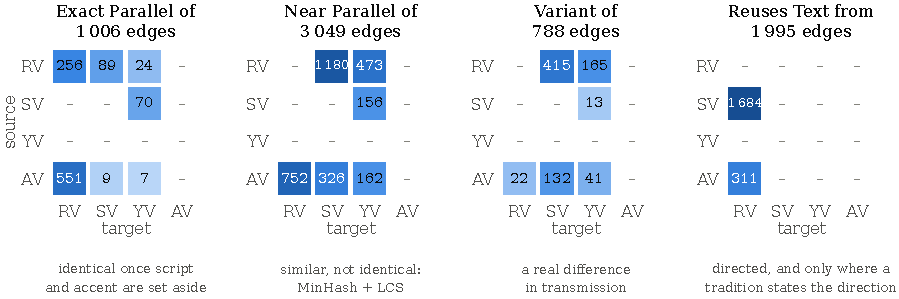
\includegraphics[width=\linewidth]{figures/fig_crossveda.pdf}
\caption{Cross-textual relationships between the four Samhit\=as, one matrix per
predicate on a shared log-scaled ramp. They are shown separately because the four
predicates assert different things; a single summed ``similarity'' matrix is the one
chart this layer exists to avoid. A dash is a measured zero, not missing data. Only
\code{REUSES\_TEXT\_FROM} is directed, and only where the direction is evidenced
(\cref{sec:reuse}).}
\label{fig:crossveda}
\end{figure}

\subsection{Formulae}
\label{sec:formula}

A \emph{formula} is a repeated multi-word span, reified as a node so that $n$
passages sharing it cost $n$ edges rather than $\binom{n}{2}$. The graph holds
4{,}825 formulae in 720 families, with 22{,}686 occurrence edges. Five bounds
control what counts, each with a stated reason:

\begin{itemize}[leftmargin=1.9em,itemsep=1pt,topsep=2pt]
\item \textbf{2 to 8 words.} One word is a lexeme --- the lemma layer already has it,
and \iast{agni} is not a formula. Above eight words a repeated span is a whole verse,
which the parallel layer already records.
\item \textbf{At least 3 distinct mantras.} Two occurrences is as often a coincidence
of sandhi as a formula.
\item \textbf{At least 12 characters.} Two very short words fold to a handful of
letters and match everywhere.
\item \textbf{At most 8\,\% of a Veda.} A span occurring in more than that share is
that Veda's grammar, not its phraseology --- and the share is computed \emph{per
Veda}, so a S\=amavedic refrain is judged against the S\=amaveda rather than against
the corpus.
\item \textbf{Ceilings} of 6{,}000 formula nodes and 120{,}000 occurrence edges, the
first because the node exists precisely to replace combinatorial edges with a hub,
and a hundred thousand hubs would defeat that.
\end{itemize}

Occurrence detection runs at two grains, and the edges record which: word-aligned
matching (20{,}577 edges) and a sandhi-insensitive substring fallback (2{,}109).
Family membership is likewise two mechanisms kept apart on the edge --- a core
grouping (1{,}828), expansion by containment (2{,}238), and a small
similarity-based extension (8) --- because the tier of a membership edge depends on
which derivation produced it, and the two directions of the mirror must be
byte-identical or a query would get a different tier depending on which way it
walked.

Contamination is a named hazard rather than an assumed absence: a documented
baseline finding records that formula nesting inflates roughly a third of
formula-bearing passages, and the containment relation is modelled explicitly so
that nesting is visible instead of double-counted.

\subsection{Ritual and material culture}
\label{sec:ritual}

The ritual layer is small but it is the clearest case in the graph for typing at the
edge rather than at the predicate, so we report it here rather than in an appendix.

The objects are modelled as distinct kinds rather than as one ``thing'' class:
103 rites, 3{,}121 ritual steps, 20 ritual roles, 21 offerings, 33 substances, 41
implements, and small populations of plants (22), animals (15), metals (7), weapons
(5) and crops (5). The step layer is the large one, and it is source-explicit: a
rite's procedural steps are what a source prints, and all 3{,}121 carry that layer.
An earlier pass had filed those steps under a generic ``Other'' category, which is a
reminder that a fine-grained vocabulary is worth nothing if the loader does not use
it.

The instructive part is the relationships. Consider two predicates:

\begin{center}\small
\begin{tabular}{@{}lrr@{}}
\toprule
Predicate & \Ltwo{} or \Lone{} & \Lfour{} \\
\midrule
\code{USED\_FOR\_RITE} & 110 & 419 \\
\code{PERFORMED\_BY}   &  16 &  16 \\
\bottomrule
\end{tabular}
\end{center}

\noindent Each carries claims of two different epistemic kinds under one name. Some
uses of a verse in a rite are derivable from what a source states about the book the
verse sits in; others are this project's reading of what the verse is for. Some
statements of who performs a rite are source-stated; an equal number are inferred.
A grade attached to the \emph{predicate} would be wrong for one population in each
row --- which is exactly the defect \cref{sec:model} describes, caught here before
it shipped rather than after.

The layer also contains the graph's only model-extracted ritual claims: 11
offering involvements, 9 ritual involvements and 3 substance involvements, 23 edges
in total, all at \Lthree{} and all excluded by a single predicate from any count a
reader wants to keep source-grounded.

Two precision controls are worth naming. Rejected candidates are retained with
reasons rather than deleted, so the offering layer ships alongside a file of
refusals. And the layer's own precision was sampled rather than assumed: a derived
metric records two figures for the ritual-context assignment --- 0.79 over every
reviewed row and 0.95 over the reproducible ones --- with a note explaining that a
single figure would have to decide whether an unreproducible row is an error or an
unknown, and that it is an unknown. That node also carries
\code{is\_human\_gold = false} and a reviewer field naming an agent, which is how
the graph says that its own quality figure is not human-adjudicated either.

\subsection{Audio, briefly}
\label{sec:audio}

Recitation audio is referenced rather than held: there is no recording node type in
the graph, and the media are linked, not mirrored. We mention the layer only because
its history contains the cleanest instance of a defect this paper's method is meant
to catch. An earlier source published one file per hymn and renumbered one
\d{R}gvedic book after a different edition's arrangement, so a key-for-key mapping
attached the wrong recitation to 55 hymns --- not a gap but a silent misalignment,
which the project's own decision record calls the worse of the two. The replacement
source was verified per verse against the stored text, and the verses it could not
verify were refused rather than mapped approximately. A separate owner decision then
made human audible review a \emph{badge} rather than a visibility gate, on the
reasoning that automated checking is not listening; the number of recordings a named
person has actually played remains small and is recorded as such.

\subsection{Direction: compilation asymmetry}
\label{sec:reuse}

Identifying that two verses are parallel says nothing about which way the borrowing
ran. The project initially asserted direction for exactly one pair --- 1{,}684
S\=amaveda-to-\d{R}gveda edges --- on a \emph{tradition's} statement that the
\=Arcika is a collection of \d{R}gvedic verses arranged for chanting, and left every
other pair undirected on the ground that asserting a direction there would be a
chronology claim. The weakness was that all 1{,}684 edges carried the identical
justification sentence: a pipeline constant that says why the class is directed and
nothing about the edge it sits on.

The replacement is a measured, per-edge signal. A borrowed verse and its source are
by construction nearly identical, so nothing about the strings can point. What points
is the company each verse keeps. A compiler assembles a unit out of verses drawn from
elsewhere, so its unit is largely made of counterparts, and those counterparts are
scattered across many units of the other corpus; a composer's hymn is not made of
anything, and only some of its verses happen to have been taken. For each side,
measured on that side's own containing unit:
\[
  \text{share} = \frac{|\{v \in U : v \text{ has a counterpart}\}|}{|U|},
  \qquad
  \text{dispersion} = |\{\,U' : \text{some counterpart lies in } U'\}|.
\]
Direction is asserted from the high-share side to the low-share side, and only when
share $\ge 0.5$ and the margin between sides is $\ge 0.25$.

Two preconditions refuse pairs before the measure runs, both on measured grounds.
\emph{\d{R}gvedic mediation}: if two verses in different corpora are both
counterparts of the same \d{R}gvedic verse, those corpora share \d{R}gvedic text
rather than each other's --- measured at 96.1\,\% of Atharvaveda/S\=amaveda pairs,
95.4\,\% of S\=amaveda/Yajurveda and 83.3\,\% of Atharvaveda/Yajurveda, against
0.0\,\% of \d{R}gveda/Yajurveda. \emph{Unit granularity}: the measure is a ratio over
a structural unit, and the median containing unit holds 9 verses in the \d{R}gveda,
4 in the Atharvaveda, 3 in the S\=amaveda --- and 44 in the Yajurveda, whose smallest
container here is the \iast{adhy\=aya}. A share over a 44-verse unit is not the same
instrument as a share over the three-verse unit that is modal in the S\=amaveda
(281 of its 458 containing units hold exactly three verses, whatever the addressing
calls them), so every Yajurvedic pair is
refused.

Finally the instrument is only allowed to speak in a scope where it demonstrates
both power (at least 100 directed verdicts) and internal consistency (at least
90\,\% pointing the same way). The scope table is the interesting output:

\begin{center}\small
\begin{tabular}{@{}lrrl@{}}
\toprule
Scope & Directed & Consistency & Outcome \\
\midrule
\d{R}gveda/S\=amaveda, whole pair & 1{,}212 & 0.991 & accepted, SV $\to$ RV \\
Atharvaveda/\d{R}gveda, whole pair & 480 & 0.763 & \textbf{rejected} \\
Atharvaveda/\d{R}gveda, k\=a\d{n}\d{d}a 20 & 322 & 0.966 & accepted, AV $\to$ RV \\
\d{R}gveda/Yajurveda, whole pair & 325 & 0.532 & \textbf{rejected} \\
\bottomrule
\end{tabular}
\end{center}

\noindent The method recovers the tradition's own claim about the S\=amaveda
independently, at 0.991; it localises the Atharvavedic case to k\=a\d{n}\d{d}a 20,
which is exactly the book known to be largely \d{R}gvedic; and it declines the two
scopes where it cannot separate the sides. Four typed refusal codes record which
precondition or floor rejected a pair.

\subsection{What the corpus's structure does \emph{not} establish}

One negative result belongs here because it disciplines the whole layer. The
S\=amaveda has the highest undirected parallel coverage of the four works held
here, at 1{,}677 of 1{,}844 verses --- 90.9\,\%, against 34.8\,\% for the
next-placed Yajurveda --- and that figure is routinely read as self-evident
confirmation that the S\=amaveda borrows. Against a degree-preserving permutation
null over 400 draws, \d{R}gveda/S\=amaveda containment is $6.69\times$ observed
against $5.72\times$ expected from corpus size alone: an excess of only $1.17\times$.
The recorded conclusion is that no size-independent structural signature in anything
the project holds distinguishes borrower from source for any pair --- which is
precisely why direction had to come from compilation asymmetry and from a tradition's
explicit statement, rather than from coverage.

The same audit exposed a typing defect of the kind \cref{sec:model} describes: the
parallel edges carry an evidence surface of \code{SANSKRIT}, which is true of the
pairing and false of the direction. The pairing is derived from the Sanskrit; the
direction is not.

% generated by figures-src/make_tables.py -- do not edit
\begin{table}[tb]
\centering
\caption{Cross-textual relationships between mantras, by predicate and work pair.
The four predicates are deliberately not collapsed into one ``similar to'': they
assert different things, and the strongest, \code{REUSES\_TEXT\_FROM}, is directed only
where a tradition states the direction (\cref{sec:reuse}). Pairs are shown as
source~$\to$~target.}
\label{tab:reuse}
\small
\begin{tabularx}{\linewidth}{@{}lr>{\raggedright\arraybackslash}X@{}}
\toprule
Predicate & Edges & By work pair \\
\midrule
\code{EXACT\_PARALLEL\_OF} & 1{,}006 & \footnotesize AV$\to$RV~551, RV$\to$RV~256, RV$\to$SV~89, SV$\to$YV~70, RV$\to$YV~24, AV$\to$SV~9, AV$\to$YV~7 \\
\code{NEAR\_PARALLEL\_OF} & 3{,}049 & \footnotesize RV$\to$SV~1{,}180, AV$\to$RV~752, RV$\to$YV~473, AV$\to$SV~326, AV$\to$YV~162, SV$\to$YV~156 \\
\code{VARIANT\_OF} & 788 & \footnotesize RV$\to$SV~415, RV$\to$YV~165, AV$\to$SV~132, AV$\to$YV~41, AV$\to$RV~22, SV$\to$YV~13 \\
\code{REUSES\_TEXT\_FROM} & 1{,}995 & \footnotesize SV$\to$RV~1{,}684, AV$\to$RV~311 \\
\bottomrule
\end{tabularx}
\end{table}


\subsection{A refused layer}

For completeness: a semantic-resemblance layer was proposed and refused before
import, on a re-implemented lexical control it could not beat
(\cref{sec:eval-baseline}). Zero assertions were written. Its absence from
\cref{tab:reuse} is a decision, not an omission.

\section{Case Studies}
\label{sec:cases}

\subsection{S\=amavedic notation: gating the withholding, not only the release}
\label{sec:case-samaveda}

The S\=amaveda is the Veda of chant, and its \=Arcika verses are printed in some
witnesses with svara marks indicating the melodic treatment of each syllable. This
layer is the project's sharpest test of the evidence model, for three reasons: the
marks are genuinely source-explicit, decoding them into pitch would be genuinely
interpretive, and the coverage is genuinely partial.

\paragraph{What was admitted.} 1{,}136 of the 1{,}844 \=Arcika verses carry an
accented witness (\cref{tab:samaveda}, \cref{fig:samaveda}), imported as a second
\code{TextVersion} of
the verse's own text in the role \code{PARALLEL\_TEXT}, never replacing the primary
text. We verified all of this against the live store: 1{,}136 accented parallel text
versions against 1{,}844 primary ones, and 25{,}542 tone marks on the accented rows.
Coverage is published as four figures rather than one --- \textsc{chanda} 471/585,
\textsc{aranya} 31/55, \textsc{mahanamnya} 3/10, \textsc{uttara} 631/1194 --- because
a single total of 1{,}136 hides which part of the \=Arcika a reader can and cannot
see notation for.

\paragraph{What was refused, and how the refusal is enforced.} The marks are recorded
as data and never decoded. The Kauthuma decipherment authority is not held, and a
study of a different school's chant was deliberately not applied. The refusal is
enforced at four levels rather than stated once: the row schema pins the payload to a
closed set of thirteen field names and checks that none of them names a pitch; the
predicate is the ordinary \code{HAS\_TEXT\_VERSION}, and a melodic predicate is
verified absent from the store's type table; the migration plan declares six explicit
refusals; and a live test scans every property key on the witness for pitch
vocabulary, permitting exactly one match --- the property that \emph{records} the
refusal. We confirmed the outcome: no melodic relationship type exists in the graph,
and the property \code{notation\_is\_interpreted\_into\_pitch} is present on all
1{,}136 witnesses with the value \emph{false}. A first version of that scan flagged
the guard as the thing it guards against, which is a small but exact illustration of
how hard it is to write a check that means what it says.

\begin{figure}[tbp]
\centering
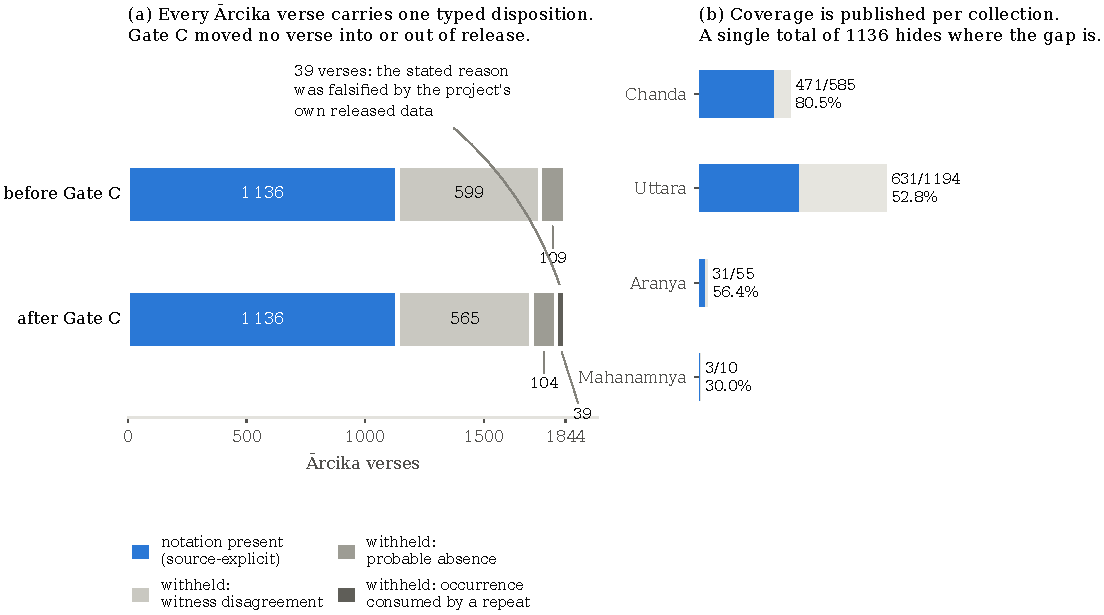
\includegraphics[width=\linewidth]{figures/fig_samaveda.pdf}
\caption{The S\=amavedic notation layer before and after the adversarial gate.
\textbf{(a)} Every one of the 1{,}844 \=Arcika verses carries exactly one typed
disposition. Gate~C moved no verse into or out of release; it added a third
withheld class and moved 39 verses into it, because the reasons those rows stated
were falsified by the project's own released data. \textbf{(b)} Coverage is
published per collection rather than as one total, because a total of 1{,}136 hides
which part of the \=Arcika a reader can and cannot see notation for.}
\label{fig:samaveda}
\end{figure}

% generated by figures-src/make_tables.py -- do not edit
\begin{table}[tb]
\centering
\caption{S\=amavedic notation: every one of the 1{,}844 \=Arcika verses carries
exactly one typed disposition, so a reader can never mistake a withheld verse for a
verse the tradition does not notate. The third withheld class did not exist until an
adversarial gate falsified the stated reasons of 39 rows.}
\label{tab:samaveda}
\small
\begin{tabularx}{\linewidth}{@{}lr>{\raggedright\arraybackslash}X@{}}
\toprule
Disposition & Verses & \\
\midrule
notation present, source-explicit & 1{,}136 & \footnotesize the witness prints marks on this verse \\
\quad withheld: near line, witness disagreement & 565 & \footnotesize needs philological adjudication \\
\quad withheld: no near line, probable absence & 104 & \footnotesize the witness may not carry the verse \\
\quad withheld: occurrence consumed by a repeat & 39 & \footnotesize \textbf{added by Gate C} (\cref{sec:case-samaveda}) \\
\midrule
\textbf{Total} & \textbf{1{,}844}
& \footnotesize verses with no disposition at all: \textbf{0} \\
\bottomrule
\end{tabularx}
\end{table}


\paragraph{Gate C, and the negative control.} The layer was audited by a gate
implemented separately from the pipeline that produced it, and the separation is
explicit: Gate C names the fields it refuses to read --- including the pipeline's own
tone-stripped text and its quality report --- and re-implements the declared
normalisation from the manifest's prose, using Unicode character categories rather
than the artefact's integer ranges. Eight attacks ran at full coverage over 6{,}232
row-evaluations.

The design feature we want to draw out is the second attack. Having re-derived each
verse's canonical text and found it aligned on 1{,}136 of 1{,}136, the gate then ran
the \emph{same} fold against the \emph{next} verse, and got 0 of 1{,}136. The gate's
own statement is the methodological point: the aligned result is only evidence to the
extent that this one is near zero. An agreement measurement without a negative
control does not distinguish a working method from a trivially satisfiable one.

\paragraph{The finding: 39 withheld rows whose reason the repository disproved.} Seven
attacks survived. The seventh did not, and it is the one that attacked the project's
own withholdings. 708 verses were withheld under two declared reason classes: 599
saying a near line exists so the difference needs philological adjudication, and 109
saying the accented witness plausibly does not carry the verse at all. The attack
observed that both claims are falsifiable from the repository itself --- if a
withheld verse's exact normalised text is \emph{released}, with notation, on a
coreferent twin elsewhere in the \=Arcika, then the witness demonstrably carries the
text and neither stated reason is the true mechanism.

Thirty-nine verses failed this test: 34 from the witness-disagreement class and 5
from the probable-absence class, each with at least one released twin carrying
byte-identical normalised text. The true mechanism was then measured rather than
guessed: of 202 repeated-text groups, 153 have every member released, so the witness
does print a repeated verse more than once and the harvest does find both lines.
Where only one member is released, the single order-consistent occurrence was
consumed by the earlier verse and the later one had no line left. That is line
exhaustion on a coreferent repeat --- neither an absence from the witness nor a
philological disagreement.

\paragraph{What changed, and what deliberately did not.} A third withheld class was
declared, \code{WITNESS\_OCCURRENCE\_CONSUMED\_BY\_A\_COREFERENT\_REPEAT}, and the
39 rows were moved into it; we read the corrected distribution off the live graph as
565 / 104 / 39, summing to the unchanged 708. \emph{No verse moved from withheld to
released, and no notation value was invented.} The gate's reasoning is that the
notated string belongs to the coordinate the witness printed it at, so copying a
twin's marks onto another verse would be inventing notation --- only the stated
reason changes. The original reason text is preserved verbatim on each corrected
row, and because the staging directory is a checksum-sealed artefact whose generator
is not in the repository, the correction was applied as an overlay rather than an
edit, leaving all twelve manifest checksums valid.

Finally, the failing run is preserved on disk and a test asserts that it still
records 39 defects, so the finding cannot be erased by regenerating only the passing
run. Gate C also declined to count the artefact's own pre-existing adversarial
sample, on the ground that it targets a different population and was run by the same
pass that produced it.

\paragraph{Why the gate existed at all.} An owner decision had released the notation
layer from an unrelated audio gate on four conditions, three of which measured met.
The fourth required that ``existing validation gates pass'' --- and the eligibility
record showed one gate \code{UNKNOWN} and the other \code{NOT\_RUN}. The condition
was recorded as unmet, with the reasoning that reading ``gates'' as the single gate
that already existed would clear the board by narrowing a word, and that the
conservative reading is the one that cannot manufacture a closure. A second owner
ruling confirmed the conservative reading, so the two gates were built rather than
the word narrowed. The newly built gate immediately landed a real defect.

\subsection{Translation: coverage is a kind, not a boolean}
\label{sec:translation}

Three separate mechanisms in this project once answered the question ``is this verse
translated?'' and all three answered it by testing for a translation edge. That test
was correct while every translation was a one-to-one rendering of its own verse, and
it stopped being correct the moment anything else was admitted.

\paragraph{Why alignment is hard here.} Five failure modes were measured, and none is
a data-quality problem that better sources would fix. The editions do not share a
verse spine: for a run of \emph{dvipada vir\=aj} hymns the canonical verses are single
hemistichs while the translator numbers the four-p\=ada group as one unit, printing
five units against ten verses. The available translation may be of a \emph{different
recension}: the standard English S\=amaveda is R\=a\d{n}\=ayan\=\i ya on its own
translator's preface, while this corpus is Kauthuma, and nine avenues were searched
without finding a public Kauthuma \=Arcika translation. Position cannot substitute,
because the offset between the two orders drifts monotonically from 0 to $-81$. The
source's own printed labels are sometimes wrong --- one book prints the sequence
23, 24, 23, 26, a misprint for 25. The corpus repeats itself, so ``same English,
different verse'' is normal rather than a defect; two of the packet's own duplication
tests were wrong for exactly that reason before the third was right. And a
translation can be present, correctly typed, and still invisible to a reader's edge
test, which is how a range alignment went unseen.

\paragraph{The typed model.} The replacement is two closed vocabularies and one
refusal. A \emph{coverage kind} says what a translation gives a verse --- dedicated,
range, container, or reused --- and is explicitly not rankable; the classifier
\emph{raises} on an unrecognised alignment level rather than defaulting, because
defaulting is how a fourth kind would silently be reported as a verse's own
translation. A \emph{verse coverage state} says what a verse has, in eight values of
which three are negative and distinguish genuinely different situations
(\cref{tab:coverage}). Alignment confidence is a six-valued typed vocabulary rather
than a number pretending to be a probability; the largest class, covering 17{,}095 of
18{,}427 renderings, is \code{MACHINE\_ALIGNED\_NO\_PER\_ROW\_CONTROL}, which names
its own weakness.

% generated by figures-src/make_tables.py -- do not edit
\begin{table}[tb]
\centering
\caption{Translation coverage as a typed state rather than a boolean. Each of the 20{,}210 mantras carries exactly one terminal state, so an absence always arrives with its reason attached. The two \code{UNCOVERED} states are distinct on purpose: one says a translated identical parallel exists elsewhere in the corpus, the other says nothing reaches the verse at all. The S\=amavedic column is the reason the distinction was built.}
\label{tab:coverage}
\small
\begin{tabular}{@{}lrrrrr@{}}
\toprule
Verse coverage state & RV & AV & YV & SV & Total \\
\midrule
\code{DEDICATED\_TRANSLATION} & 10{,}322 & 5{,}715 & 1{,}950 & 0 & 17{,}987 \\
 & \multicolumn{5}{@{}l@{}}{\footnotesize its own 1:1 English rendering} \\[2pt]
\code{RANGE\_TRANSLATION\_ANCHOR} & 30 & 34 & 0 & 0 & 64 \\
 & \multicolumn{5}{@{}l@{}}{\footnotesize anchors a print unit spanning it and others} \\[2pt]
\code{RANGE\_COVERED} & 36 & 52 & 0 & 0 & 88 \\
 & \multicolumn{5}{@{}l@{}}{\footnotesize carries no edge; named in another verse's span} \\[2pt]
\code{CONTAINER\_TRANSLATION} & 158 & 0 & 0 & 0 & 158 \\
 & \multicolumn{5}{@{}l@{}}{\footnotesize only rendering is aligned to a hymn} \\[2pt]
\code{REUSED\_RENDERING} & 0 & 21 & 0 & 173 & 194 \\
 & \multicolumn{5}{@{}l@{}}{\footnotesize another corpus's rendering of identical Sanskrit} \\[2pt]
\code{UNCOVERED\_REUSABLE\_PARALLEL\_AVAILABLE} & 0 & 6 & 0 & 1{,}488 & 1{,}494 \\
 & \multicolumn{5}{@{}l@{}}{\footnotesize nothing reaches it, but a translated identical parallel exists} \\[2pt]
\code{UNCOVERED\_NO\_RENDERING\_REACHES\_IT} & 6 & 11 & 25 & 183 & 225 \\
 & \multicolumn{5}{@{}l@{}}{\footnotesize nothing reaches it, and no parallel does} \\[2pt]
\midrule
\textbf{Total} & \textbf{10{,}552} & \textbf{5{,}839} & \textbf{1{,}975} & \textbf{1{,}844} & \textbf{20{,}210} \\
\bottomrule
\end{tabular}
\end{table}


\paragraph{What the S\=amavedic column shows.} 1{,}488 S\=amavedic verses are
uncovered \emph{but} have a translated identical parallel elsewhere in the corpus;
183 are uncovered with no parallel at all; and 173 carry a reused \d{R}gvedic
rendering admitted only on Sanskrit verified character-identical. The last of these
is the case the model was built for. Those 173 are visible to a reader, and they are
counted in no S\=amavedic translation figure: the code holds two frozen sets, one for
``English reaches the reader'' and one for ``independent English exists'', differing
by exactly the reused class, and records that a total reporting 173 English
translations for the S\=amaveda is wrong --- a mistake an earlier draft of the
staging made before the reuse column was checked. The independent-English count for
the S\=amaveda is zero.

\paragraph{Two disciplines worth naming.} First, the product shipped \emph{before}
the data: the import plan was built and hashed but deliberately not executed in the
commit that introduced the typed model, on the reasoning that the interface must be
able to represent a range and a reused rendering before such rows land, not
afterwards. Second, the campaign restated one of its own headline figures
\emph{downward} on purpose. Narrowing ``translated'' to mean a verse's own rendering
moved the \d{R}gvedic figure from 10{,}502 to 10{,}479, and a test now asserts the
range population beside it so that the narrowing cannot pass as a regression.

\paragraph{And a defect this found.} A prior import had attached 25 renderings to the
wrong verses, precisely because two editions did not share a verse spine and the
guard reported the mismatch as ``missing'' rather than as a spine divergence. The
rows were re-anchored and the readback was clean --- but the more useful artefact is
the reason code introduced alongside:
\code{SOURCE\_EDITION\_VERSE\_DIVISION\_DIFFERS}, which is now one of six typed
rejection reasons rather than an unexplained absence.

\section{Evaluation}
\label{sec:eval}

Evaluation of a construction method like this one is awkward, because the thing to be
evaluated is not a single model's output but a discipline. We report five kinds of
measurement: the graph's scale and internal integrity, the distribution of epistemic
types, precision against an external reference set, the outcomes of adversarial
gates, and one downstream question-answering benchmark. We then state at length what
none of these establish.

\begin{figure}[tbp]
\centering
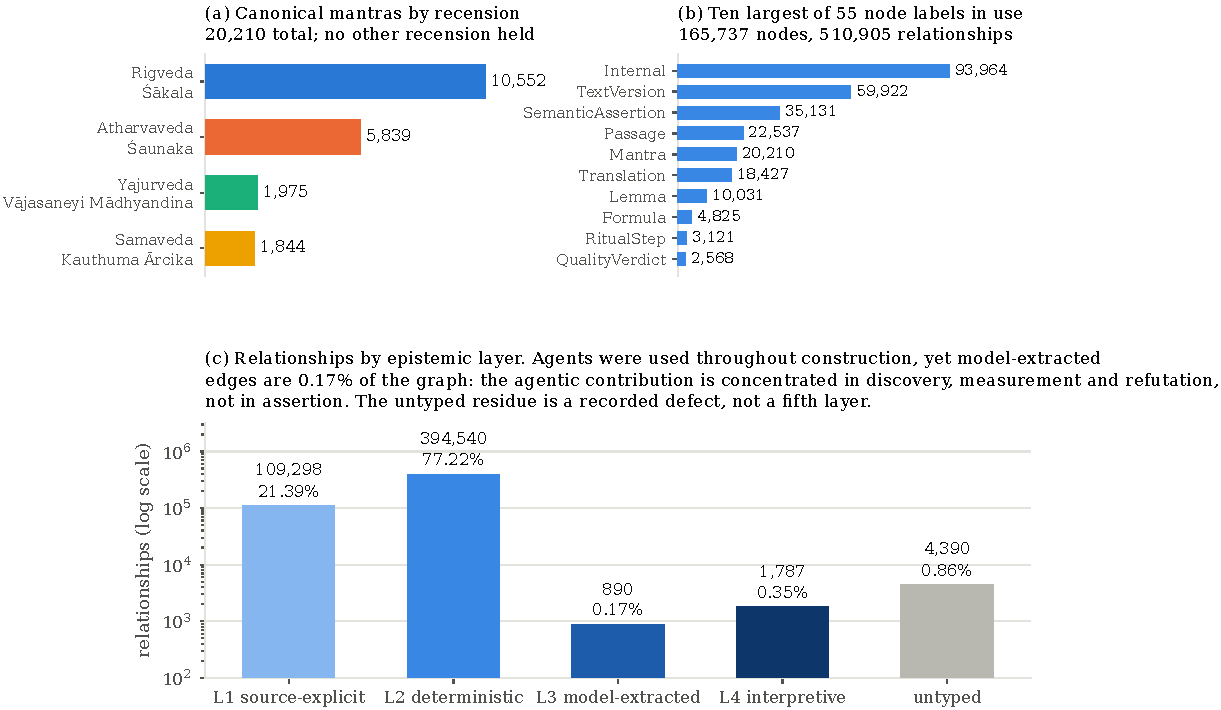
\includegraphics[width=\linewidth]{figures/fig_corpus_and_epistemic.pdf}
\caption{Corpus, graph scale, and the distribution of epistemic types.
\textbf{(a)} The canonical corpus is four named recensions, not ``the Vedas''.
\textbf{(b)} The ten largest node labels; \code{Internal} is a marker on non-public
objects, not a domain type. \textbf{(c)} The paper's central measurement, on a log
scale: agents were used continuously throughout construction, and model-extracted
relationships are 0.17\,\% of the graph. The untyped residue is a recorded defect in
the grading contract, not a fifth layer. Measured on the live store at commit
\code{6bf220c}.}
\label{fig:corpus-epistemic}
\end{figure}

\subsection{Scale and integrity}

% generated by figures-src/make_tables.py -- do not edit
\begin{table}[tb]
\centering
\caption{The fourteen largest node labels and relationship types, of 55 labels
in use and 81 relationship types.
A further label, \code{SourceArtifact}, is declared in the store's token table but
carries no nodes.}
\label{tab:labels}
\small
\begin{tabular}{@{}lr@{\hskip 2em}lr@{}}
\toprule
Node label & Nodes & Relationship type & Edges \\
\midrule
\code{Internal} & 93{,}964 & \code{MENTIONS\_LEMMA} & 154{,}261 \\
\code{TextVersion} & 59{,}922 & \code{HAS\_TEXT\_VERSION} & 59{,}922 \\
\code{SemanticAssertion} & 35{,}131 & \code{HAS\_SEMANTIC\_ASSERTION} & 35{,}131 \\
\code{Passage} & 22{,}537 & \code{ASSERTION\_PREDICATE} & 32{,}938 \\
\code{Mantra} & 20{,}210 & \code{MENTIONS\_ENTITY} & 28{,}122 \\
\code{Translation} & 18{,}427 & \code{ABOUT\_CONCEPT} & 24{,}861 \\
\code{Lemma} & 10{,}031 & \code{USES\_FORMULA} & 22{,}686 \\
\code{Formula} & 4{,}825 & \code{CONTAINS} & 22{,}537 \\
\code{RitualStep} & 3{,}121 & \code{HAS\_TRANSLATION} & 18{,}427 \\
\code{QualityVerdict} & 2{,}568 & \code{HAS\_RISHI} & 17{,}889 \\
\code{RoleFiller} & 2{,}052 & \code{MENTIONS\_DEVATA} & 17{,}165 \\
\code{DerivedMetric} & 1{,}485 & \code{HAS\_CHANDAS} & 16{,}298 \\
\code{PadaParallelGroup} & 1{,}434 & \code{HAS\_DEVATA} & 10{,}558 \\
\code{QAIssue} & 915 & \code{SHARES\_FORMULA\_WITH} & 6{,}148 \\
\bottomrule
\end{tabular}
\end{table}


At the frozen commit the graph holds 165{,}737 nodes and 510{,}905 relationships
across 55 node labels in use and 81 relationship types
(\cref{fig:corpus-epistemic}, \cref{tab:labels}). Of the nodes, 71{,}773 are public
and 93{,}964 carry the internal marker. Every one of the 71{,}773 public nodes has a
non-null public identifier and the identifiers are distinct.

Integrity is gated rather than asserted, and we ran the gates rather than quoting
the project's certification of them. That distinction turned out to matter.

The eleven scorecard gates all read zero: internal leakage, ungraded edges, nodes
without a label, orphan entities, signature violations, undeclared relationship
types, interpretive claims graded other than the weakest tier, claims and metrics
pointing at passages, orphan public nodes, and labels falsely declared unpopulated.

\textbf{The twenty live invariants do not all pass.} Running the suite at the frozen
commit gives 17 ok, 1 warning and \emph{2 failures}:

\begin{center}\small
\begin{tabular}{@{}llr@{}}
\toprule
Severity & Invariant & Edges \\
\midrule
\textsc{fail} & \code{edges\_without\_grade\_basis} & 165{,}788 \\
\textsc{fail} & \code{edges\_without\_attribution\_precision} & 19{,}598 \\
\textsc{warn} & \code{assertions\_without\_predicate\_edge} & 2{,}193 \\
\bottomrule
\end{tabular}
\end{center}

\noindent So 32.5\,\% of edges cannot say \emph{why} they carry the grade they
carry, and 3.8\,\% do not say whether they are a per-verse claim, an inherited
label, a textual mention, or not an attribution at all. Both invariants are declared
at failing severity by the repository itself.

We report this prominently because of how we came to it. An earlier draft of this
paper asserted that all twenty invariants passed, on the authority of the project's
release certification --- which recorded that state truthfully at an earlier census.
We had not run the suite. An adversarial reviewer of this manuscript ran it in one
command and the claim fell. That is precisely the failure the paper is about: a
report was trusted where a measurement was available, by the authors of a paper
arguing that reports are not evidence. It is recorded in
\code{supplementary/peer\_review.md} and we have not smoothed it away here.

What does hold as a universal quantifier, verified: no edge without a quality tier
(510{,}905 of 510{,}905), no unlabelled node, no product node reaching a diagnostic
node, no attribution-precision value outside the declared enumeration, no work
without a scope statement, and no predicate carrying more than one run identifier.

\paragraph{One coverage gap we report rather than round away.} The quality tier is
present on 100.00\,\% of edges. The \emph{knowledge layer} is present on 99.14\,\%:
4{,}390 edges carry no layer, and they are not scattered --- they are 4{,}079
\code{HAS\_PARALLEL\_PADA} edges and 311 \code{REUSES\_TEXT\_FROM} edges. Worse than
their number is the grade they carry: \emph{all 4{,}390 are \code{TIER\_B}}, the tier
the model defines as ``a reproducible rule derived it''. An edge whose origin the
graph does not record is therefore presented to a reader as reproducibly derived.
The tier-from-layer mapping is also not the total bijection \cref{sec:model}
describes: besides the documented candidate rule (292 model-extracted edges at
\code{TIER\_D}), 2{,}469 deterministically derived edges carry \code{TIER\_D} and 36
source-explicit edges carry \code{TIER\_B}. This is a real residual defect in the
graph-wide typing contract, not a fifth layer, and the
percentages in \cref{tab:layers} are computed over all 510{,}905 edges rather than
over the typed subset, so the gap is visible rather than divided away.

\subsection{The distribution of epistemic types}
\label{sec:eval-distribution}

The central measurement of this paper is \cref{tab:layers}. Model-extracted
relationships number 890, or 0.17\,\% of the graph; interpretive claims number
1{,}787, or 0.35\,\%. The remaining 98.6\,\% is either what a source states
(21.39\,\%) or what a reproducible rule derives from what a source states
(77.22\,\%).

\paragraph{The ratio depends on the population, so we give four.} A reviewer of
this manuscript observed, correctly, that 0.17\,\% is the smallest of several
defensible figures and that quoting only it overstates the result. The denominator
of 510{,}905 includes populations no extraction method could ever author ---
154{,}261 lemma mentions, 59{,}922 text-version links, 22{,}537 containment edges
and 18{,}427 translation links, 255{,}147 in all. Over the 255{,}758 edges that
remain once that plumbing is removed, the model-extracted share is 0.35\,\%. Over
the semantic
assertion layer alone --- the population where a model is actually the proposing
mechanism --- it is 2{,}459 of 35{,}131, or \textbf{7.0\,\%}. And if one counts
every edge whose existence is owed to a model proposal rather than only those
carrying the layer, the figure is higher again.

All four are true of different questions. The one the paper's argument needs is not
the smallest but the one over the population at risk: \textbf{where a model could
assert, it authored 7.0\,\% of the assertions, and none of them was promoted}. We
keep 0.17\,\% as the graph-wide figure because a consumer filtering the whole store
is filtering the whole store, and we state the others here so that the choice of
denominator is the reader's rather than ours.

At node level the same shape holds: of 165{,}737 nodes, 2{,}459 carry the
model-extracted layer, all of them \code{SemanticAssertion} nodes with derivation
\code{MODEL\_EXTRACTION}. The remaining 32{,}672 semantic assertions are derived by
morphological rule over a published scholarly annotation or from a treebank
dependency relation, and the project's own code refuses to blend the two totals,
on the ground that a blended figure states a confidence about all 35{,}131
assertions that is true of neither population.

\paragraph{And 89\,\% of the model layer is not wired.} Of the 2{,}459
model-extracted assertions, \textbf{2{,}193 carry no \code{ASSERTION\_PREDICATE}
edge at all} --- their predicate is a property but not a relationship, so
predicate-level traversal cannot see them. The repository's own invariant suite
reports this at warning severity, and it is the third adversarial finding from an
earlier round that was never remediated. It bears directly on the figure above: had
those assertions been wired as the deterministic derivations are, the
model-extracted edge count would be 890 plus 2{,}193, and the graph-wide share
would be roughly 0.6\,\% rather than 0.17\,\%. Part of what the headline ratio
measures is a wiring defect rather than a discipline.

Two further measurements characterise how much the semantic layer withholds. Of the
35{,}131 assertions, 28{,}734 carry \code{roles\_withheld}, and only 341 are
three-slot complete --- that is, fewer than 1\,\% of the semantic assertions assert a
full agent--predicate--patient frame. The layer is overwhelmingly a predicate layer
with the role slots deliberately empty (\cref{sec:failure}, F2).

\begin{figure}[tbp]
\centering
\resizebox{0.95\textwidth}{!}{% GENERATED by figures-src/fig_indra.py -- do not edit by hand.
% Queried live; selection criteria are in that script's docstring.
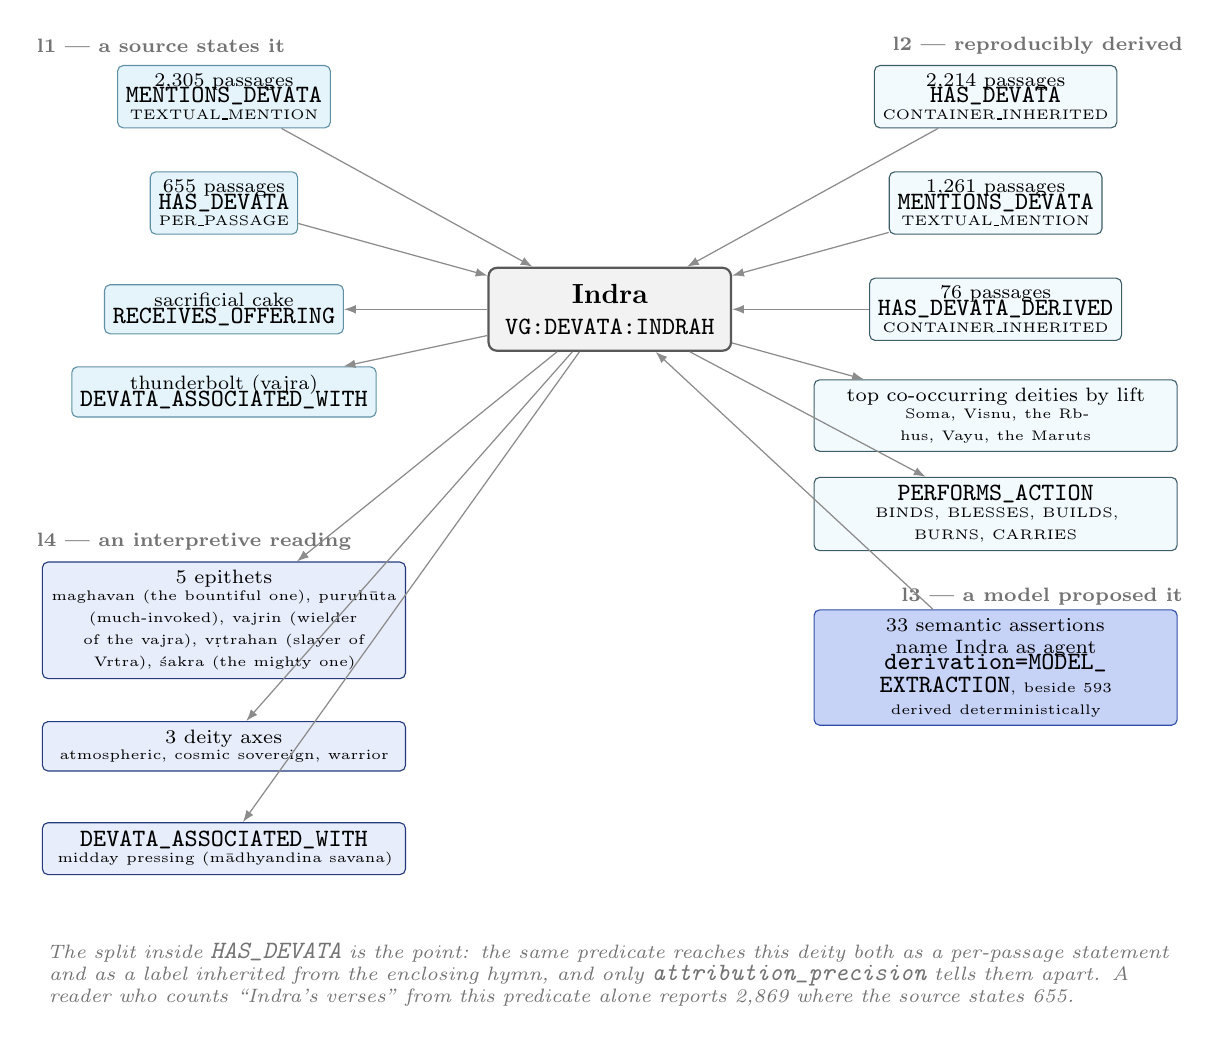
\begin{tikzpicture}[
  font=\footnotesize, every node/.style={align=center},
  hub/.style={draw=black!65, line width=0.8pt, rounded corners=3pt,
              fill=black!5, inner sep=6pt, font=\bfseries},
  nd/.style={draw=black!40, rounded corners=2pt, inner sep=3pt,
             font=\scriptsize, fill=white, line width=0.4pt},
  l1/.style={nd, fill=SkyBlue!22, draw=SkyBlue!70!black},
  l2/.style={nd, fill=SkyBlue!10, draw=SkyBlue!45!black},
  l3/.style={nd, fill=RoyalBlue!30, draw=RoyalBlue!75!black},
  l4/.style={nd, fill=RoyalBlue!12, draw=RoyalBlue!55!black},
  e/.style={-{Latex[length=1.5mm,width=1.1mm]}, draw=black!45,
            line width=0.45pt},
  el/.style={font=\tiny\itshape, text=black!60, inner sep=1.2pt,
             fill=white},
  sec/.style={font=\scriptsize\bfseries, text=black!55},
]
\node[hub] (indra) at (0,0) {Indra\\[-1pt]\scriptsize\mdseries \code{VG:DEVATA:INDRAH}};
\node[sec, anchor=west] at (-7.4,3.35) {\textsc{l1} --- a source states it};
\node[l1] (a0) at (-4.9,2.70) {2{,}305 passages\\[-2pt]\code{MENTIONS\_DEVATA}\\[-2pt]\tiny TEXTUAL\_MENTION};
\draw[e] (a0) -- (indra);
\node[l1] (a1) at (-4.9,1.35) {655 passages\\[-2pt]\code{HAS\_DEVATA}\\[-2pt]\tiny PER\_PASSAGE};
\draw[e] (a1) -- (indra);
\node[l1] (c10) at (-4.9,0.00) {sacrificial cake\\[-2pt]\tiny \code{RECEIVES\_OFFERING}};
\draw[e] (indra) -- (c10);
\node[l1] (c11) at (-4.9,-1.05) {thunderbolt (vajra)\\[-2pt]\tiny \code{DEVATA\_ASSOCIATED\_WITH}};
\draw[e] (indra) -- (c11);
\node[sec, anchor=east] at (7.4,3.35) {\textsc{l2} --- reproducibly derived};
\node[l2] (b0) at (4.9,2.70) {2{,}214 passages\\[-2pt]\code{HAS\_DEVATA}\\[-2pt]\tiny CONTAINER\_INHERITED};
\draw[e] (b0) -- (indra);
\node[l2] (b1) at (4.9,1.35) {1{,}261 passages\\[-2pt]\code{MENTIONS\_DEVATA}\\[-2pt]\tiny TEXTUAL\_MENTION};
\draw[e] (b1) -- (indra);
\node[l2] (b2) at (4.9,0.00) {76 passages\\[-2pt]\code{HAS\_DEVATA\_DERIVED}\\[-2pt]\tiny CONTAINER\_INHERITED};
\draw[e] (b2) -- (indra);
\node[l2] (cooc) at (4.9,-1.35) [text width=44mm] {top co-occurring deities by lift\\[-2pt]\tiny Soma, Visnu, the Rbhus, Vayu, the Maruts};
\draw[e] (indra) -- (cooc);
\node[l2] (acts) at (4.9,-2.60) [text width=44mm] {\code{PERFORMS\_ACTION}\\[-2pt]\tiny BINDS, BLESSES, BUILDS, BURNS, CARRIES};
\draw[e] (indra) -- (acts);
\node[sec, anchor=east] at (7.4,-3.65) {\textsc{l3} --- a model proposed it};
\node[l3] (l3) at (4.9,-4.55) [text width=44mm] {33 semantic assertions name Indra as agent\\[-2pt]\tiny \code{derivation=MODEL\_EXTRACTION}, beside 593 derived deterministically};
\draw[e] (l3) -- (indra);
\node[sec, anchor=west] at (-7.4,-2.95) {\textsc{l4} --- an interpretive reading};
\node[l4] (ep) at (-4.9,-3.95) [text width=44mm] {5 epithets\\[-2pt]\tiny maghavan (the bountiful one), puruhūta (much-invoked), vajrin (wielder of the vajra), vṛtrahan (slayer of Vrtra), śakra (the mighty one)};
\draw[e] (indra) -- (ep);
\node[l4] (ax) at (-4.9,-5.55) [text width=44mm] {3 deity axes\\[-2pt]\tiny atmospheric, cosmic sovereign, warrior};
\draw[e] (indra) -- (ax);
\node[l4] (c4) at (-4.9,-6.85) [text width=44mm] {\code{DEVATA\_ASSOCIATED\_WITH}\\[-2pt]\tiny midday pressing (mādhyandina savana)};
\draw[e] (indra) -- (c4);
\node[font=\scriptsize\itshape, text=black!55, text width=14.2cm, align=left] at (0,-8.45) {The split inside \code{HAS\_DEVATA} is the point: the same predicate reaches this deity both as a per-passage statement and as a label inherited from the enclosing hymn, and only \code{attribution\_precision} tells them apart. A reader who counts ``Indra's verses'' from this predicate alone reports 2{,}869 where the source states 655.};
\end{tikzpicture}
}
\caption{One entity, four epistemic layers: the neighbourhood of Indra, queried
live. High-cardinality passage predicates are aggregated by (predicate, layer,
attribution precision); low-cardinality typed neighbours are drawn individually and
capped. Selection criteria are stated in the generating script. The split inside
\code{HAS\_DEVATA} is the point of the figure.}
\label{fig:indra}
\end{figure}

\subsection{Precision against an external reference set}
\label{sec:gold}

No human gold standard exists for any VedGraph claim. We use the project's own term,
\code{INDEPENDENT\_SOURCE\_ADJUDICATED\_REFERENCE\_SET}, for what does exist, and we
use it strictly.

\paragraph{What it is.} VedGraph's lexical and mention claims were machine-compared
against the Treebank of Vedic Sanskrit \citep{hellwig2020vedic}, a published,
human-validated annotation of 27{,}182 sentences. Verse addresses were established by
de-accented, de-spaced skeleton containment inside the cited hymn with a similarity
floor of 0.62 and a requirement that the winner beat the runner-up by 0.06; the
alignment was then checked for monotonicity (5{,}541 adjacent pairs, 90 backwards
jumps at 1.62\,\%, with both sides of every jump quarantined and 176 sentences
dropped) and confirmed against an independent lemma annotation already in the graph.
The resulting set is 3{,}951 rows folding 11{,}210 adjudicated claims, with 805 rows
refused for an ambiguous margin and 77 below the floor. It reaches 3{,}072 of the
20{,}210 mantras.

\paragraph{What it measures.} On the lexical layers the reference set gives precision
in the range 0.982--0.994 with recall 0.443--0.543. The precision figure is the
useful one; the recall figure is bounded by the treebank's own coverage rather than
by the layer's behaviour.

\paragraph{What it is not.} The project's own statement is that the human annotation
is of the \emph{Vedic text}, not of VedGraph's claims, and that the verdict was
derived from it mechanically --- one step removed from human review of the project's
own assertions, and the strongest thing obtainable without commissioning an
annotator. The reference set cannot decide aboutness or referent. It reaches zero
S\=amavedic mantras, so the 11{,}380 enrichment edges on the S\=amaveda --- every
outgoing edge from an \=Arcika mantra other than text, translation and containment
--- are not
merely unannotated but, in the project's word, unscoreable.

\paragraph{Zero human annotation, verified.} Across 695 rows in the gold directory
there are no human annotations. The 120-row semantic scaffold is empty --- every row
\code{UNANNOTATED}, zero entities and zero relations. The 575-row theonym set is
labelled \code{MODEL\_ADJUDICATED} by a single model. We confirmed the consequence in
the live store: no edge carries a human-reviewed provenance on any of four candidate
properties, the only node bearing an \code{is\_human\_gold} property carries the value
\emph{false}, and the strongest review state present is \code{MODEL\_ADJUDICATED} on
613 edges. The 1{,}166 quality-verdict nodes each carry an explicit
\code{not\_human\_gold\_because} property.

The single most informative number here is a negative one. Of 74 theonym rows the
treebank could reach, 72 were decidable, and the model adjudication agreed with the
human annotation on 54 --- \textbf{75\,\%}. A quarter divergence on the only
independent test available is the reason the set is not promoted to gold, and it is
the best available estimate of what single-model adjudication is worth in this
domain.

\paragraph{Agent agreement is reported, and is never called accuracy.} Inter-run and
inter-agent agreement figures exist and are labelled as such: a 12-replica
cross-agent calibration reaching a mean Jaccard of 0.832 on assertion sets but exact
set agreement on only 1 of 12; a two-run stability check whose verdict is recorded as
\code{POLICY\_STABILITY\_ONLY\_NOT\_ACCURACY}; and a pair of earlier model runs
disagreeing on 91.6\,\% of 120 mantras. The only Cohen's $\kappa$ in the repository
(0.567 four-way, 0.366 binary) is model against model. Every such report carries the
project's standing banner that model self-agreement is not accuracy.

\subsection{Adversarial gate outcomes}
\label{sec:eval-gates}

Fourteen domains passed through a three-gate structure (\cref{sec:gates}). The
outcomes worth reporting are the failures, since a gate that never fails is not
evidence. Across the campaign, gates rejected or forced the withdrawal of: 13{,}187
elements that the domain rules said never to import; 5{,}930 edges over-written by a
first import attempt; 12{,}033 nodes left unreachable by a second; 102 curated
display labels silently overwritten by a third; 33 metre assertions whose object was
not a metre; 49{,}179 of 51{,}231 semantic role fillers; and the stated reasons of 39
withheld S\=amavedic verses (\cref{sec:case-samaveda}).

Three structural features of the regime are worth separating from its results.
First, several gates were built only after an owner declined to narrow the word
``gates'' to mean the one gate that already existed; the newly built gate then landed
a real defect on its first run. Second, a failing run is preserved on disk and pinned
by a test asserting its defect count, so a finding cannot be erased by regenerating
only the passing run. Third, at least one gate was found to be incapable of failing:
it computed its set of declared relationship types as the union of the ontology and
the graph, then asked which graph types were missing --- and so reported zero
undeclared types for an entire wave while eleven predicates went unclassified.

\subsection{A baseline that the project's own semantic layer lost to}
\label{sec:eval-baseline}

One genuine controlled comparison exists. A semantic-resemblance layer was proposed,
and before importing it the project re-implemented a purely lexical control --- a
character-4-gram similarity --- and evaluated both against 279 adjudicated pairs. The
lexical control reached an \mbox{AUC} of 0.754, and no semantic candidate beat it.
The layer was refused: zero assertions imported, the graph unmutated, the outcome
recorded as \code{VERIFIED\_ZERO \vgslash  REFUSED}.

Two details make this more useful than a bare negative result. The prior run's
reported control figure did not reproduce --- 6 of 370 pairs matched exactly --- and
the project's response was to withdraw the carry-over argument entirely rather than
reconcile the numbers, recording that no prior number travels forward. And the
adjudication labels for those 279 pairs are themselves \mbox{LLM}-produced, with 162
of 486 pairs left \code{UNADJUDICATED\_QUOTA\_EXHAUSTED}; the comparison is therefore
between two candidate generators judged by a third model, which is what makes it a
usable relative ranking and not an absolute precision figure.

\subsection{Downstream: a question-answering benchmark}
\label{sec:eval-ask}

The graph supports a retrieval-and-synthesis interface, and a 60-question benchmark
evaluates it. We report it as downstream evidence that the evidence typing survives
into use, not as a language-model evaluation.

The question set is frozen and hash-pinned, hand-authored in three cohorts (18
demonstration, 10 adversarial including two prompt-injection probes, 32 closure) over
eight categories including four deliberately unanswerable questions. The freezing
policy is explicit: questions are not edited in response to a poor answer, because a
benchmark that moves when the model stumbles measures nothing.

Grading is hybrid and contains no \mbox{LLM} judge. The mechanical half is
deterministic --- all 60 evidence packets replayed from the live store to identical
item counts, 304 citations audited, every integer in the prose matched against the
packet's numeric facts, Sanskrit runs classified for provenance, eight regex safety
probes --- and the composition refuses to run if a hard gate fails. The adjudicated
half is a human reading each answer against its replayed packet.

The final state is 39 \code{SUPPORTED\_CORRECT}, 4 \code{PARTIAL\_CORRECT}, 17
\code{INSUFFICIENT\_EVIDENCE\_CORRECTLY\_REFUSED}, 0 \code{MISLEADING} and 0
\code{HALLUCINATED}. Seventeen refusals out of sixty is the number we would draw a
reader's attention to: the interface declines more than a quarter of the questions
put to it, which is the behaviour the evidence typing is for.

The caveats are severe and are the project's own: a single provider and model, one
sample per question, no repeated sampling, no cross-provider comparison, a single
unnamed adjudicator, and therefore no inter-annotator agreement. Three answers were
truncated by an output-token cap. The Sanskrit quote auditor over-reports, flagging
59 runs across 23 answers with zero fabrications among them, so readers of those 23
answers are warned away from wording that was never presented as a quotation.

\subsection{Reproducibility}
\label{sec:reproducibility}

Reproducibility was measured rather than asserted, by re-running. The canonical
corpus builds are byte-reproducible: rebuilding produces identical artefacts, and the
identity scheme reproduces all 22{,}537 passage identifiers exactly
(\cref{sec:identity}). A separate check verified that two independent source builds
produce a public-identifier key set identical to the live graph's.

We state the limit plainly, because the repository does. \textbf{A fresh clone cannot
bootstrap a certified graph.} The corpus artefacts, registries, staging evidence,
gates and build scripts are in version control; the loaded Neo4j store is not, several
source artefacts cannot be redistributed under their recorded rights, and the
generator of at least one sealed staging artefact is not in the repository at all ---
which is why a defect in it had to be corrected by an overlay rather than by editing
the artefact. \Cref{sec:data-availability} states which parts are available on what
terms.

\section{Failure Analysis and Threats to Validity}
\label{sec:failure}

\subsection{Failure-driven refinement}

The project's most useful output, for the purposes of this paper, is its record of
being wrong. We report the cases in a uniform shape --- what was produced, what
detected the defect, why the first method failed, what changed, and the
methodological rule that followed --- because the rule is the transferable part.
\Cref{tab:failures} summarises; the text treats the six most instructive.

% Hand-authored: this table carries judgement (what detected what, and which rule
% follows), not measurement, so it is not generated from the fact freeze. Every
% figure in it is cross-checked against the artefact cited in Appendix F.
\begin{table}[tb]
\centering
\caption{Failure ledger. Each row is a case in which the project's own output was
withdrawn, refused or corrected. ``Detected by'' names the mechanism that caught it,
which is the column that matters: in no case was the defect found by the process that
produced the output.}
\label{tab:failures}
\footnotesize
\begin{tabularx}{\linewidth}{@{}l>{\raggedright\arraybackslash}X
                             >{\raggedright\arraybackslash}p{27mm}
                             >{\raggedright\arraybackslash}X@{}}
\toprule
& What was withdrawn or refused & Detected by & Rule that followed \\
\midrule

F1 & 41{,}796 relationships deleted in one revision; 30{,}539 retired in the next,
     including 21{,}246 concept edges resting on one English keyword
   & a question no stored field could answer
   & if two populations need different trust and no field separates them, the field
     is missing \\

F2 & 49{,}179 of 51{,}231 semantic role fillers
   & sampling: 24.8\,\% wrong, unresponsive to tuning
   & an error rate that will not tune is an unsupported layer, not a
     miscalibrated one \\

F3 & an entire image-transcription corpus; then the refusal's own ``monotone
     improvement'' claim
   & inter-reader agreement 0.505 over 204 units; then re-reading the series
   & a refusal is a claim and gets the same scrutiny as an assertion \\

F4 & a deity-community partition, then the decisive argument \emph{for} refusing it
   & a second pass reading the project's own curation notes
   & do not import the standard scholarly view as the graph's model and then grade
     the graph against it \\

F5 & a release candidate, with all 11 scorecard gates green
   & a registry with 84 of 85 entries open and no closed state expressible
   & a gate measures a property; completeness is a property of a registry \\

F6 & nothing --- a \emph{correct} restoration of 30{,}266 nodes degraded the product
   & a legibility measurement at a fixed display budget
   & completeness and legibility are different objectives \\

F7 & the stated reasons of 39 withheld S\=amavedic verses
   & a gate built to attack the withholding, with a negative control
   & gate the refusals, not only the assertions \\

F8 & a semantic-resemblance layer, before import: 0 assertions written
   & a re-implemented lexical control at \mbox{AUC} 0.754 that nothing beat
   & re-implement the baseline rather than carrying its number forward \\

F9 & 33 metre assertions whose object was a bracket fragment, not a metre
   & a closed-world check on the object vocabulary
   & resolving into a contaminated vocabulary is not resolution \\

F10 & 13{,}187 imported elements the domain rules excluded; 5{,}930 edges
      over-written; 12{,}033 nodes orphaned; 102 curated labels overwritten
    & readback comparing rows \emph{sent} against rows \emph{landed}
    & an importer's own success report is not evidence \\

\bottomrule
\end{tabularx}
\end{table}


\paragraph{F1. A layer deleted 41{,}796 of its own edges, and its successor retired
30{,}539 more.} The second revision of the knowledge model deleted 41{,}796
relationships that the same revision had created in error. The third then withdrew
30{,}539 further edges, of which 21{,}246 were concept-attribution edges that had
fired on a single keyword in Griffith's 1896 English. The detection was not a test
but a question: what surface was this evidence read off? Because the answer was not
recorded anywhere, the edges were indistinguishable from edges matched on the
Sanskrit, and they carried an identical grade. \emph{Rule:} if two populations
require different trust and no stored field separates them, the field is missing,
and its absence is a defect of the same order as a wrong value. The evidence-surface
axis (\cref{sec:model}) exists because of this case.

\paragraph{F2. Ninety-six per cent of the role layer withdrawn.} A semantic role
layer had asserted 51{,}231 role fillers. Sampling put the wrong-filler rate at
24.8\,\%. Repair was attempted first and failed on measurement: widening the gate
moved the error only to 24.3\,\% at a cost of eighteen recall points, with per-role
residue ranging from 11.4\,\% on goal to 31.2\,\% on location. The layer was reduced
to the 2{,}052 fillers resting on a published treebank's own labels; 28{,}734
assertions were stamped \code{roles\_withheld} with a reason, and 15{,}704 withdrawn
rows were staged as a verification queue rather than deleted. The project's summary
is the finding: the \d{R}gveda now has a predicate layer and no role layer at all,
because it has no parse. \emph{Rule:} when a measured error rate does not respond to
tuning, the layer is not miscalibrated but unsupported, and withdrawal is the correct
repair.

\paragraph{F3. A corpus refused on measured fidelity, then the refusal's own
reasoning corrected.} An independent image transcription of an 1856 Atharvavedic
edition was built and then refused: exact agreement between two independent readings
of the same material was 0.505 over 204 units. What makes the case instructive is
what happened to the \emph{explanation}. A report had described the agreement series
as a monotone climb that had ``risen every time''; the actual series was 0.00, 0.26,
0.485, 0.505, 0.542, 0.522, and it later fell again to 0.500 over 272 units. The
trend claim was withdrawn with the observation that asserting a trend from five
points is the same overgeneralisation the paragraph was written to correct, committed
inside the correction itself. A second claim --- that the accent layer was
unrecoverable --- was also withdrawn, because one worker had captured it with a
reproducible method; the gap was a convention divergence, not a capability limit.
\emph{Rule:} a refusal is a claim and needs the same scrutiny as an assertion.

\paragraph{F4. A refusal whose decisive argument was wrong.} A deity-community
partition was refused on the ground that every method separated two names for one
deity. Re-examination overturned the refusal's reasoning rather than the refusal: the
project's registry \emph{deliberately} holds those two names apart, with
high-confidence curation notes and no variant edge between them. The agent had
imported the standard scholarly view as the graph's model and then graded the
partition defective for respecting the project's own curation. The refusal was
reformalised on a different, measurable basis and the original claim was recorded as
withdrawn in the required form --- original claim, withdrawal, reason. A related
figure was corrected in both directions at once: an imbalance is tenfold over all 214
deities and 7.9-fold over the 157 eligible ones, peaking in different books.
\emph{Rule:} neither figure is wrong; they differ by population, so a population must
be named beside any ratio.

\paragraph{F5. Every gate green, and the release still refused.} At the close of a
completeness campaign the scorecard read 11/11, dependency state was current, and
every test suite passed --- and the verdict was
\code{DATA\_COMPLETENESS\_NOT\_COMPLETE}, release candidate \emph{no}. The cause was
that the gap registry had no closed state: 84 of 85 entries were open, there was no
closure vocabulary, and no field could hold one. The decisive individual finding was
a registry entry recording ``closed via the Wayback Machine, 944 of 961'' against a
graph holding exactly the pre-closure figure, with all 2{,}254 accepted staging rows
targeting real mantras and none carrying a translation. \emph{Rule:} a gate measures
a property; completeness is a property of a \emph{registry}, and a registry with no
terminal state cannot express it. The closure vocabulary in \cref{tab:gaps} was added
in response.

\paragraph{F6. The completeness campaign made the product worse.} A correct
restoration of 30{,}266 previously dropped semantic-assertion nodes doubled the size
of the exported interactive artefact and pushed the share of the public graph that is
apparatus --- evidence records and passages rather than entities --- to roughly
81\,\%. Measured at a display budget of 40 neighbours, the entry for Indra spent 21
seats on passages and evidence records and 6 on other deities. Nothing about the
curation had changed; the corpus had. \emph{Rule:} completeness and legibility are
different objectives, and a graph that improves on the first can regress on the
second without any individual claim becoming false.

% generated by figures-src/make_tables.py -- do not edit
\begin{table}[tb]
\centering
\caption{The gap registry at \code{6bf220c}. Until a late campaign the registry had
no closed state at all, so every gate could be green while completeness was
unresolvable (\cref{sec:failure}); the closure vocabulary below was added to make
termination expressible.}
\label{tab:gaps}
\small
\begin{tabular}{@{}lr@{}}
\toprule
Status & Entries \\
\midrule
\code{CLOSED\_DERIVED} & 53 \\
\code{CLOSED\_SCOPE\_DECISION} & 14 \\
\code{BLOCKED\_EXTERNAL\_SOURCE\_UNAVAILABLE} & 7 \\
\code{CLOSED\_VERIFIED\_ZERO} & 5 \\
\code{NEEDS\_AUDIBLE\_REVIEW} & 3 \\
\code{CLOSED\_NOT\_APPLICABLE} & 2 \\
\code{CLOSED\_SOURCE\_ACQUIRED} & 1 \\
\midrule
\textbf{Total} & \textbf{85} \\
\multicolumn{2}{@{}l}{\footnotesize of which closed by some route: \textbf{75}} \\
\bottomrule
\end{tabular}
\end{table}


\subsection{What the adversarial rounds found in each other}

Five hostile rounds ran over the release candidate. The pattern worth reporting is
that later rounds found defects in earlier rounds' own work: one round closed two
critical findings that the same round's hostile pass had raised against itself. A
related case is the public-identity collision, in which 30{,}266 semantic-assertion
nodes carried no assertion identifier and fell through to their source passage's
canonical key --- collapsing two public objects onto one and silently dropping
assertion-to-passage edges as self-edges.

The generalisable observation is that an agent auditing its own output finds less
than a differently-instructed agent auditing the same output, and that the gap is
large enough to matter at this scale. We are careful not to overstate this: the
agents are not independent in the statistical sense. They share a model family, and
in several cases the same family produced both the artefact and its audit.

\subsection{Threats to validity}
\label{sec:threats}

\paragraph{Construct: recension scope.} Every absence measured here is an absence
from four named recensions. The Kr\d{s}\d{n}a Yajurveda, the Paippal\=ada
Atharvaveda, all four S\=amavedic \iast{g\=ana} collections and every post-Sa\d{m}hit\=a
layer are absent. A reader who reads ``the Atharvaveda does not say X'' as a claim
about the Atharvavedic tradition will be wrong.

\paragraph{Construct: the Atharvavedic corpus is a working corpus.} The Atharvavedic
text is held as a reference-only, working-private digital corpus carrying an explicit
assertion that its lineage is \emph{not} an independent transcription of the printed
edition it descends from. Its mantra count, 5{,}839, stands against an attested total
of roughly 5{,}977, and the divergence is recorded as open research rather than
resolved.

\paragraph{Internal: agent non-independence and correlated error.} The adversarial
design assumes that an attacking agent fails differently from the agent it attacks.
Where both are the same model family, that assumption is weak, and a shared blind
spot would be invisible to the whole regime. We have no measurement of this. The one
relevant datum is discouraging: single-model adjudication agreed with published human
annotation on only 75\,\% of the 72 decidable cases where the two could be compared.

\paragraph{Internal: a single human decision-maker.} The human arm of the workflow is
one person, who is also the project's author and the author of this paper. Owner
rulings are recorded with their reasoning, which makes them auditable, but they are
not independent of the project's goals, and there is no second reader anywhere in the
pipeline.

\paragraph{Internal: thresholds are chosen, not learned.} The alignment floor of
0.62, the margin of 0.06, the near-parallel similarity cut, and the formula-length
bounds are all set by hand. Some were set after inspecting their effects, which is a
form of fitting to the corpus.

\paragraph{Internal: normalisation is lossy by construction.} The lateral fold merges
two phonemically distinct letters because two source conventions use the same code
point for both (\cref{sec:normalisation}). This is documented and was measured, but
it means a small number of comparisons are structurally incapable of distinguishing
two words.

\paragraph{Conclusion: what the layer distribution does and does not show.} The
0.17\,\% figure is a faithful measurement of what is \emph{in} the graph. It is not a
measurement of how much agents contributed to the project, which was very large, nor
of how much they contributed to what the graph \emph{says}, since an agent that finds
and removes a wrong edge shapes the graph without appearing in it. We intend the
figure to answer only the question of authorship of claims.

\paragraph{Conclusion: no absolute precision for the semantic layer.} The reference
set cannot decide aboutness or referent, reaches 3{,}072 of 20{,}210 mantras, and
reaches no S\=amavedic mantra at all. We therefore report no precision figure for the
semantic assertion layer as a whole, and we regard any such figure derived from
model adjudication as unsupported.

\paragraph{External: generality.} The method was developed on one corpus by one
person over seventeen days. The corpus is unusually favourable in one respect --- it
is closed, small enough to enumerate, and equipped with a traditional metadata
apparatus --- and unusually hostile in another, in that its normalisation is
genuinely contested. We discuss what we think transfers in \cref{sec:discussion}.

\paragraph{Internal: two failing invariants, and what they mean for the rest.} Two
of the twenty live invariants fail (\cref{sec:eval}): 165{,}788 edges carry no grade
rationale and 19{,}598 carry no attribution precision. The second is the more
serious for this paper's argument, because \cref{sec:model} presents attribution
precision as a graph-wide axis and 3.8\,\% of edges do not carry it. Neither
failure affects the layer distribution --- the quality tier is present on every
edge and the knowledge layer on 99.14\,\% --- but a reader should treat any
statement here about a \emph{universal} property as holding for the properties we
name as verified and not beyond them.

\paragraph{Internal: thresholds were selected on the corpus they are evaluated on.}
The near-parallel floor is justified by inspecting what a lower floor produces on
this corpus; the alignment floor and margin are likewise hand-set. There is no
held-out set anywhere in the project. Every precision figure in \cref{sec:eval} is
therefore optimistically biased by an amount we have not measured.

\paragraph{Internal: recall of the candidate generator is not zero-loss.} The
banding is described in the source as tuned so that every pair at 0.44 or better is
proposed. For 32 bands of 3 rows the standard locality-sensitive-hashing curve puts
the probability of proposing a pair at similarity 0.44 at roughly 0.94, not 1. We
report the source's claim as the source's and do not adopt it: the layer's recall
below the floor is unmeasured.

\paragraph{Construct: a single decider with a stated commitment.} The human arm of
the workflow is one person, who is the project's author, this paper's author, and
--- as the acknowledgments record --- someone with a devotional relationship to the
subject matter. We raise this here and not only there, because it is a conflict of
a different kind from the goal-alignment problem already noted: a reader is
entitled to ask whether the owner rulings that decide scope and withholding are
independent of a commitment to the material. We do not think the record shows them
distorted --- the rulings that matter most are refusals --- but we cannot establish
it from inside, and no second reader exists anywhere in the pipeline.

\paragraph{Provenance gaps.} A registry statement and the projected graph can drift.
We found one live instance while preparing this paper: the S\=amavedic
\code{Work} node's completeness property still carries a pre-import sentence
asserting that zero translations are released, where the registry file that is the
source of truth was updated at the import to state the position precisely --- that
the 173 renderings are reused \d{R}gvedic English on verified-identical Sanskrit and
are counted in no S\=amavedic translation figure. The registry is right and the
projection is stale. The general hazard is that prose-valued properties are not
covered by the invariants that cover typed ones.

\section{Discussion}
\label{sec:discussion}

\subsection{What agents were actually good for}

The measurement in \cref{sec:eval-distribution} invites a deflationary reading:
agents contributed 0.17\,\% of the graph's edges, so they barely mattered. That
reading is wrong, and the reason is worth stating precisely. Agents were the
project's instrument for four things that deterministic code could not do and a
single human could not do at this scale.

\emph{Reading heterogeneous sources into a schema.} Deciding that a particular TEI
file has no editorial-alternative elements despite its header's boilerplate, or that
a translator's preface commits him to a different recension, is reading. It is
error-prone, it is cheap for a model, and it is checkable afterwards.

\emph{Generating candidates cheaply enough to be thrown away.} The project's most
valuable candidate sets are the ones that were discarded. Discarding 49{,}179 role
fillers is only a rational move if producing them was cheap; the same is true of the
semantic-resemblance layer that never landed. Agentic generation changes the
economics of refusal.

\emph{Cross-file reconciliation.} Several of the most consequential defects ---
a registry claiming a closure the graph did not hold, a report citing a path whose
file did not contain the digests described, a gate computing a set that made its own
question unanswerable --- are inconsistencies between artefacts that no single test
covered. Finding them is a reading task over hundreds of files.

\emph{Adversarial probing with a stated attack.} The Gate C case
(\cref{sec:case-samaveda}) is the clearest instance. The attack --- ``if a withheld
verse's exact normalised text is released on a coreferent twin, the stated reason is
false'' --- is a hypothesis about the project's own explanations, and it is the kind
of hypothesis an agent can be asked to generate and then required to test
mechanically.

What agents were \emph{not} used for is equally definite: they did not decide what
was true. The promotion gate is a frozen set of trust classes, the candidate status
is the only status a model may write, and the unlocked-predicate set is empty by
construction.

\subsection{What should stay deterministic}

Three functions, on the evidence here, should never be delegated.

\textbf{Identity.} A model asked whether two verses are the same verse will answer,
and its answer will be a similarity judgement wearing an identity claim's clothes.
Identity in VedGraph is a pure function of declared coordinates, and the one place
where a normalised label \emph{is} an identity input is scoped to the candidate layer
and named as such.

\textbf{Promotion.} The transition from candidate to accepted must be a property of
the pipeline, not of the proposer, and it must be expressed as data so that it can be
audited. Expressing it as a reviewer's convention would have failed: we observed a
case where a completed review had simply never been applied, leaving 149 assertions
live that a reviewer had not accepted, and the graph's count of reviewed edges at
zero not because nothing had earned it but because the earning was never recorded.

\textbf{Arithmetic over the graph.} Every count in this paper is a query. The
project's own Q38 failure (\cref{sec:eval-ask}) shows why: a synthesised answer in
which every figure was real and correctly cited was still misleading, because the
comparative words around the figures --- ``most widely'', ``largest'' --- asserted a
ranking the cited rows did not contain. Numbers can be checked mechanically;
superlatives had to be given their own rule.

\subsection{Epistemic typing as an engineering discipline}

The four-layer model is not novel as an idea --- provenance vocabularies in the
Semantic Web have expressed comparable distinctions for two decades --- but three
things about its use here seem worth transferring.

\emph{Type at the edge, not at the dataset.} A dataset-level provenance statement
cannot express that one predicate carries claims from three different kinds of
evidence. VedGraph's attribution-precision axis exists because \code{HAS\_DEVATA} is
simultaneously a per-verse statement and an inherited label, and the split
(\cref{fig:indra}) is roughly 1:3.

\emph{Give absence a type.} The strongest design decision in the project is that a
withheld row states a reason drawn from a closed class space, and that the count of
rows with no disposition at all is gated at zero. This is what made the Gate C
finding possible: you cannot falsify a reason that was never recorded.

\emph{Make the gate able to fail, and prove it.} Two gates in this project were
found to be incapable of failing, and a third's remediation shipped with ten mutant
deletions verified to turn the tests red. A passing gate is evidence only if a
failing version of the same gate has been demonstrated.

\subsection{Generalisability}

The Vedic corpus is favourable in ways that matter. It is closed and enumerable;
it carries a traditional metadata apparatus that supplies genuine source-explicit
attributions; and its recensional structure forces the scope question to be answered
explicitly. A corpus that is open-ended, or that has no equivalent of the
Anukrama\d{n}\=\i, would have a much thinner \textsc{l1}.

It is unfavourable in one way that may be more common than it looks: its
normalisation is contested, so the comparison surface is a research object rather
than a preprocessing step. Any corpus with competing transliteration conventions ---
which is most historical corpora outside the Latin alphabet --- inherits the problem
that a fold inside an identity digest is not free to change
(\cref{sec:normalisation}).

We would expect the following to transfer: separating identity from normalisation;
typing absence; expressing the promotion gate as data; requiring a negative control
in any agreement measurement; and preserving failing gate runs under test. We would
not expect the specific 0.17\,\% ratio to transfer, since it is a consequence of this
corpus having a large deterministic layer available to it.

\subsection{Relation to how such systems are usually built}

Two contrasts are worth drawing explicitly. Retrieval-augmented pipelines typically
treat provenance as a citation attached to an answer; here provenance is attached to
the claim in the store, so a consumer can filter before an answer exists. And
agentic extraction pipelines typically use a confidence score to decide what to keep;
this project refuses that on the stated ground that the score is produced by the same
process as the claim. The alternative it adopts --- per-predicate unlocking gated on
a measured precision against an external reference --- has the property that nothing
was ever unlocked, which is an honest outcome rather than a failure of the mechanism.

\section{VedAnvaya as a Research Interface}
\label{sec:interface}

The graph is exposed through a read-only \mbox{API} and a web interface called
VedAnvaya. We treat it here as evidence for one narrow claim --- that the evidence
typing survives into use --- rather than as a contribution in its own right.

The design constraint that matters is that typing is rendered \emph{at the point of
reading}, not collected on a methods page. \Cref{fig:product} shows the effect on a
single S\=amavedic verse. Four distinct epistemic situations are visible
simultaneously, each labelled in place: the svara marks are shown with the note that
they are reproduced exactly as the source edition prints them, are a record of that
edition's notation rather than a reconstructed melody, and that nothing derives a
sung realisation from them; the English is labelled a rendering \emph{via} the
verified \d{R}gvedic parallel, with a scope note stating that it is not an
independent translation of this corpus and is excluded from its translated count;
the deity named inside the verse is marked \code{PROBABLE} rather than asserted; and
the traditional ascription is marked ``not yet modelled'' rather than omitted.

\begin{figure}[tbp]
\centering
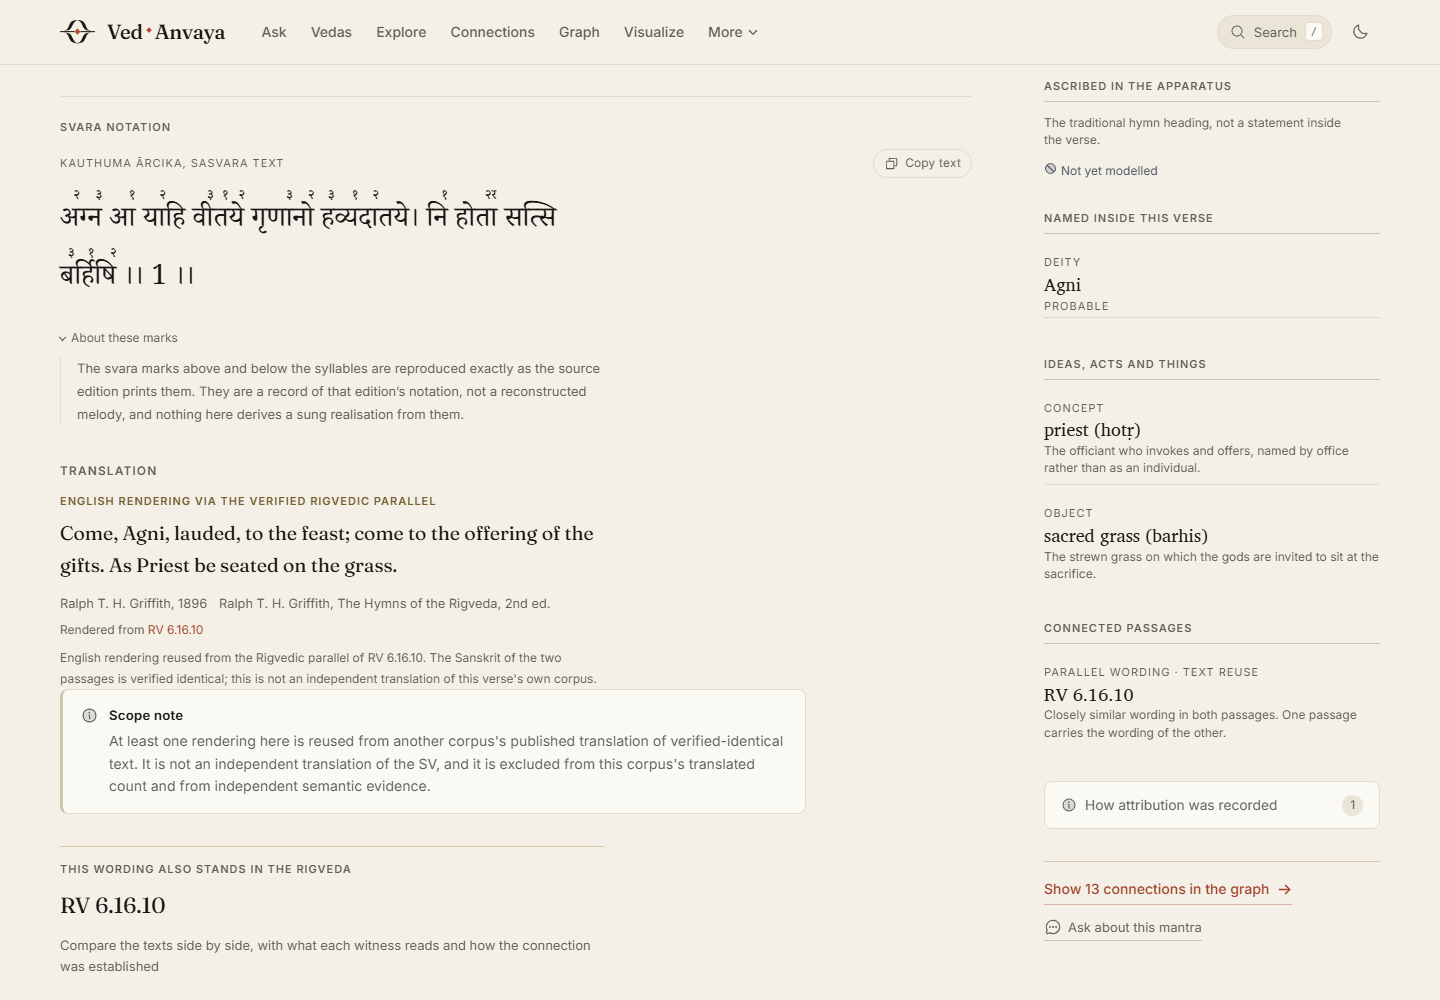
\includegraphics[width=0.96\linewidth]{figures/product/reader-samaveda-notation.png}

\vspace{6pt}
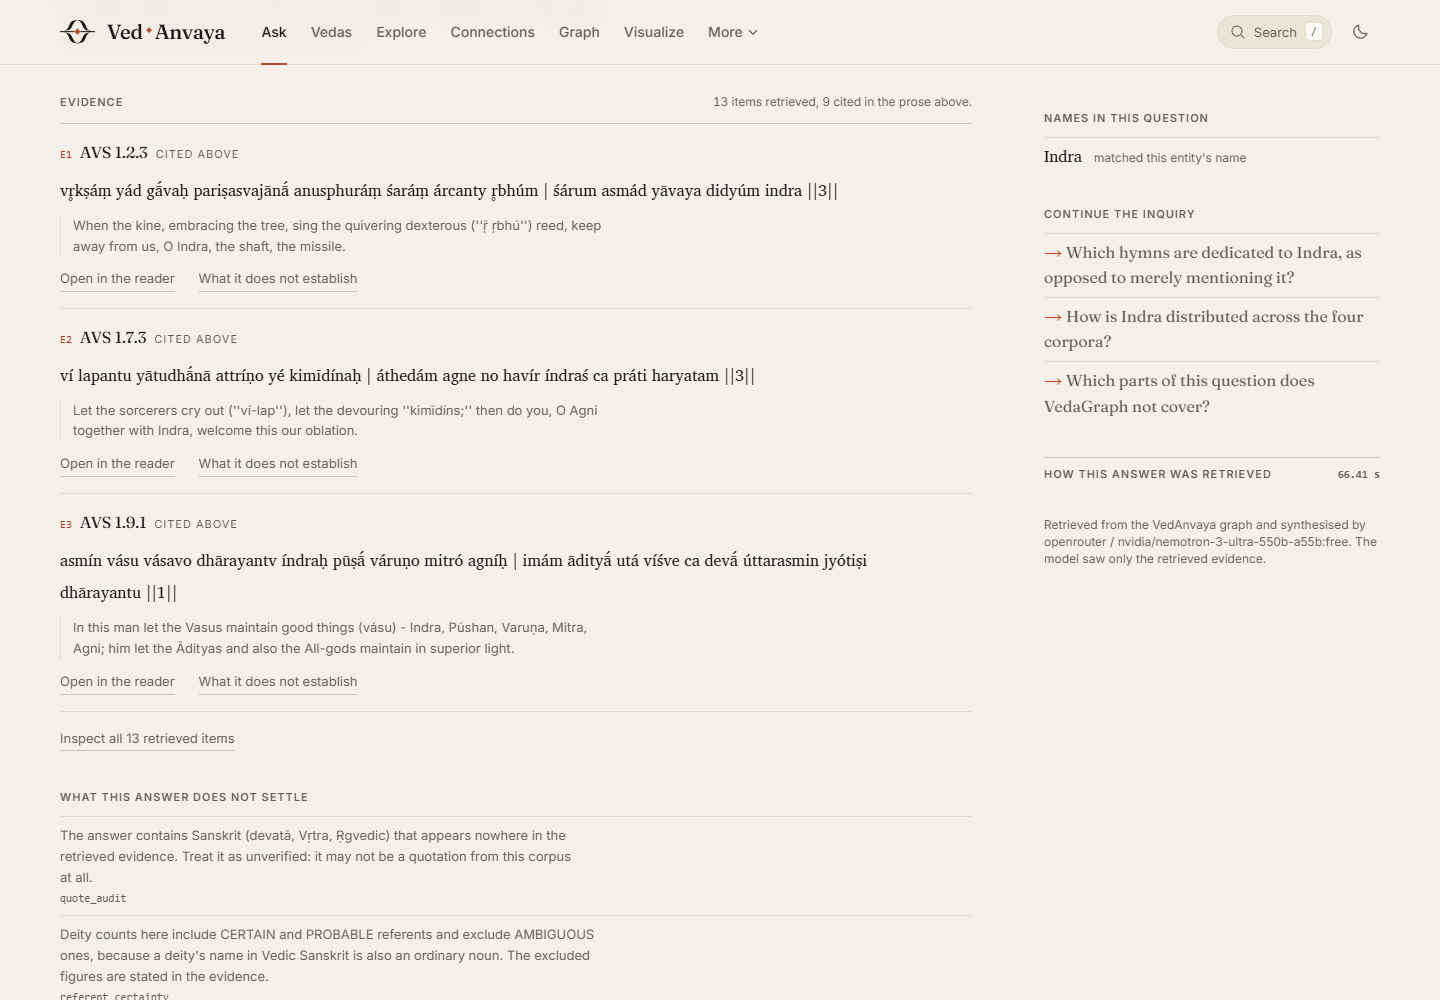
\includegraphics[width=0.96\linewidth]{figures/product/ask-evidence.png}
\caption{Evidence typing rendered where the reader is. \textbf{Top:} one
S\=amavedic verse showing four epistemic situations at once --- source-explicit
svara marks with the note that they are a record of the edition's notation and not a
reconstructed melody; an English rendering labelled as reused via a verified
\d{R}gvedic parallel and excluded from this corpus's translated count; a deity named
inside the verse marked \code{PROBABLE}; and a traditional ascription marked ``not
yet modelled'' rather than omitted. \textbf{Bottom:} the retrieved evidence beside a
synthesised answer, with a per-item ``what it does not establish'' affordance and a
closing section populated by the mechanical auditors rather than by the model.
Captured from the running product against the graph census this paper reports.}
\label{fig:product}
\end{figure}

The same discipline governs synthesis. The question-answering surface displays the
retrieved evidence beside the prose, gives each cited item an
``\emph{what it does not establish}'' affordance, and closes with a section headed
``what this answer does not settle'' that is populated by the mechanical auditors
rather than by the model --- in the case shown, a warning that the answer contains
Sanskrit appearing nowhere in the retrieved evidence, and a note that the deity
counts quoted include certain and probable referents and exclude ambiguous ones
because a deity's name in Vedic Sanskrit is also an ordinary noun.

Two behaviours are worth recording because they are unusual for an interface of this
kind and both follow from the graph rather than from interface design. The
question-answering layer declines 17 of 60 benchmark questions as insufficiently
evidenced (\cref{sec:eval-ask}). And a corpus page reports coverage as four
populations rather than one percentage, so that the S\=amaveda's zero independent
English translations is legible next to its 173 reused renderings instead of being
averaged into a single figure that would be true of neither.

We also report the interface's most instructive failure, because it is a
graph-level lesson. Restoring 30{,}266 semantic-assertion nodes --- a correct
restoration of real data --- pushed the share of the exported public graph that is
apparatus rather than entity to roughly 81\,\%, so that a visualisation of Indra's
neighbourhood at a fixed budget spent 21 of 40 slots on passages and evidence
records and 6 on other deities. Nothing had become false; the graph had simply
stopped being legible at that budget. The repair was per-class display ceilings, not
a change to the data. Completeness and legibility are different objectives, and an
interface over an evidence-typed graph has to be designed for both
(\cref{sec:failure}, F6).

\section{Limitations and Future Work}
\label{sec:limitations}

\Cref{sec:threats} treats threats to the validity of what we report. This section
treats what the artefact does not yet do, and what we think should be done next.

\paragraph{The gap a single annotator cannot close.} The decisive limitation is the
absence of human annotation (\cref{sec:gold}). Everything downstream inherits it: no
predicate can be unlocked, so no semantic assertion can be auto-accepted; no
calibration curve can exist; and the only independent check on model adjudication we
have --- 75\,\% agreement with published human annotation on 72 decidable cases ---
is a warning rather than a measurement of the layer. The useful next step is small
and specific: commission a stratified sample of a few hundred assertions annotated
by two Vedicists with an adjudication protocol, report $\kappa$, and use it to
decide whether any predicate clears the 95\,\% precision bar the policy already
defines. The machinery to consume such a set exists and is currently idling against
an empty scaffold.

\paragraph{Layer typing has a measured hole.} 4{,}390 edges carry no knowledge
layer, concentrated in two predicates (\cref{sec:eval}). This should be closed by
extending the grading contract rather than by back-filling values, since the reason
they are untyped is that the contract does not cover them.

\paragraph{Registry-to-projection drift is not gated.} We found a live instance
while writing this paper: a prose-valued scope property on a \code{Work} node that
the registry had corrected and the projection had not (\cref{sec:threats}). Typed
properties are covered by invariants; prose ones are not. A cheap fix is to hash the
registry's prose fields into the projection and gate on equality.

\paragraph{The S\=amaveda is unscoreable and partly unreachable.} No external
annotation reaches a single S\=amavedic mantra, so 11{,}380 enrichment edges on that
corpus cannot be evaluated at all, and no Kauthuma \=Arcika translation was found in
nine searched avenues. The \iast{g\=ana} corpus --- larger than the \=Arcika and the
reason the S\=amaveda is a distinct Veda --- is out of scope entirely and would need
its own work identifier, its own sources and its own rights analysis.

\paragraph{The role layer is absent, not incomplete.} Withdrawing 96\,\% of the role
fillers left a predicate layer with no argument structure
(\cref{sec:failure}, F2). Restoring it properly requires a dependency parse of the
\d{R}gveda that the project does not have; the 15{,}704 withdrawn rows are staged as
a verification queue against that future parse rather than deleted.

\paragraph{Single-provider, single-sample evaluation.} The downstream benchmark ran
one model, one sample per question, and one adjudicator. Repeated sampling, a second
provider and a second adjudicator would each be cheap and would each measure
something the present figures cannot.

\paragraph{Agent independence is assumed, not measured.} The adversarial regime's
value rests on attacking agents failing differently from the agents they attack, and
we have no evidence for that beyond the defects the regime actually found. Running
one gate under a deliberately different model family, and comparing findings, would
be a direct test and is the experiment we would most like to see run.

\paragraph{Reproducibility stops short of the store.} A fresh clone rebuilds the
corpora and re-derives every identifier but cannot produce a certified graph
(\cref{sec:reproducibility}). Publishing a loadable dump is blocked by source rights
rather than by engineering; publishing the \emph{derived, project-original} layers
separately --- the grading, the gap registry, the staging evidence --- may be
possible and would let a third party re-run the gates.

\paragraph{No cost accounting.} We report what agents produced but not what they
cost in tokens, wall-clock or money, and a method whose argument is partly economic
(\cref{sec:discussion}) ought to report that. The run artefacts contain enough to
reconstruct it for the semantic pilots; they do not for the construction work as a
whole.

\section{Conclusion}
\label{sec:conclusion}

We set out to determine whether a large historical corpus can be turned into a
provenance-aware knowledge graph with heavy \mbox{LLM}-agent involvement without
model output becoming indistinguishable from what sources actually say. The answer
this project supports is yes, but only because the constraint was implemented as
mechanism rather than as policy: a model may write exactly one lifecycle status, the
promotion gate is a frozen set of trust classes that does not contain the model's,
the predicate vocabulary is closed with its refusals named, and a cited token absent
from the packet the model was shown is a decidable fabrication.

The resulting artefact is a graph of 165{,}737 nodes and 510{,}905 relationships over
20{,}210 canonical mantras in four named recensions, in which every edge states the
epistemic layer that produced it, the tier that follows from it, the reach of the
claim over its passage, and the textual surface the evidence was read off. Because
the typing is stored rather than documented, the division of labour is measurable:
21.39\,\% of relationships are what a source states, 77.22\,\% are what a
reproducible rule derives from that, 0.35\,\% are interpretive, and \textbf{0.17\,\%
are model-extracted}.

That ratio is the paper's main empirical result, and we want it read correctly. It
does not say agents were unimportant --- they were used continuously across
seventeen days and 249 commits. It says that when the promotion path is closed, the
agentic contribution flows into discovery, measurement, reconciliation and
refutation instead of into assertion. The clearest instance is a gate built to
attack the project's own withholdings rather than its claims, which falsified the
stated reasons of 39 withheld verses using the repository's own released data, and
changed no verse's release status --- only the recorded reason. A method that can
find an error in its own explanations is doing something a method that only validates
its outputs cannot.

The project's failures support the same conclusion more strongly than its successes.
It deleted 41{,}796 of its own relationships in one revision and retired 30{,}539 in
the next; withdrew 96\,\% of its semantic role fillers rather than ship a measured
24.8\,\% error; refused an entire transcription corpus at an inter-reader agreement
of 0.505; refused a semantic-resemblance layer after a re-implemented lexical control
outperformed every candidate; and refused a release candidate while every gate was
green, because completeness turned out to be a property of a registry that had no
terminal state. Twice a refusal's own decisive argument was subsequently found wrong
and withdrawn in turn. Cheap generation makes cheap refusal possible, and refusal is
where the epistemic work happens.

What none of this establishes is the accuracy of the semantic layer. Of 35{,}131
semantic assertions, zero have been reviewed by a human; the strongest review state
in the graph is model adjudication; and on the only independent test available,
single-model adjudication agreed with published human annotation on 75\,\% of
decidable cases. The project says so in its own certification and on its public
pages, and we have been careful to say it here in the same terms. An
evidence-typed graph does not make model output true. It makes model output
\emph{visible}, and it lets a reader who does not trust it exclude it with a
predicate --- which, for scholarship over a corpus like this one, is the more useful
property.

\section*{Responsible use}
\label{sec:ethics}
\addcontentsline{toc}{section}{Responsible use}

This project puts a generative model to work on a body of text that is scripture to
living communities, and it publishes the result. Four commitments follow, and each is
implemented rather than merely stated.

\textbf{Hallucination is treated as decidable, not as a risk to be managed.} The
validator's central check is whether a token the model cited was present in the
packet the model was shown. A citation to text the model never saw is a fabricated
citation, it is mechanically decidable, and the assertion is discarded. This does not
detect a plausible-but-wrong reading of text that \emph{was} shown, which is why
model output remains a candidate regardless.

\textbf{Uncertainty is preserved rather than resolved.} Where the evidence does not
decide, the graph says so in a typed way: 28{,}734 assertions carry withheld roles,
708 S\=amavedic verses carry a withheld notation disposition in one of three declared
classes, 711 lexical tokens carry a linguistic non-resolution reason, and four
benchmark questions are expected to be refused. The system is designed so that
declining is a first-class outcome rather than a failure.

\textbf{Missing evidence is never manufactured.} Where a cue index would have needed
interpolation between anchors to yield timings, the timings were refused, because
filling the gaps means inventing a boundary. Where 466 metre rows could be resolved
into a vocabulary that was itself contaminated, the resolution was computed and still
not imported. We regard this as the single most important operational discipline in
the project.

\textbf{Interpretation is bounded, and the boundary is visible.} The predicate
vocabulary deliberately contains \code{SYMBOLIZES}, \code{REPRESENTS},
\code{IS\_GOD\_OF}, \code{MEANS} and \code{CAUSES} \emph{so that a model proposing
one is refused by name with a recorded reason}. Deity modelling is confined to what
the Sa\d{m}hit\=a verses support: identifications that belong to later exegesis are
declined individually and in writing. Musical notation is recorded as marks and never
decoded into pitch, and a test scans the stored properties to enforce it
(\cref{sec:case-samaveda}). None of this makes the graph neutral --- every
ontology encodes choices --- but it makes the choices inspectable.

A residual risk we cannot design away is authority laundering: a confident interface
over a typed graph can still be read as an oracle. The interface's mitigation is to
render the typing at the point of reading rather than in a methods page, and to
prefer refusal; whether that is sufficient is not something we can establish from
inside the project.

\section*{AI assistance disclosure}
\addcontentsline{toc}{section}{AI assistance disclosure}

AI systems were used extensively and at every stage of the work reported here:
software development, corpus inspection, candidate generation for the semantic and
entity layers, query authoring, measurement, test and gate construction, adversarial
review of the project's own output, and the drafting and editing of this manuscript.
The construction workflow described in \cref{sec:agentic} is not an incidental use of
such tools; it is the object of study.

No AI system is an author. Responsibility for the research questions, the
methodology, the interpretation of results, the claims made here and the decision to
publish rests entirely with the human author. Where a model's output entered the
artefact it did so as a typed candidate subject to the controls described in
\cref{sec:model-policy}, and the resulting population is reported rather than
absorbed: 890 relationships and 2{,}459 nodes carry the model-extracted layer, and
the graph can be queried to exclude them.

Model and runtime identities are recorded in the artefacts rather than treated as
authorship. The project's execution-runtime decision requires that the runtime that
produced a payload be recorded and never assumed, and it explicitly classifies
self-reported model identity as unattested: a receipt carries the runtime that wrote
it, and provider-attested build metadata is marked unavailable because no provider
supplies it. The reason given is directly relevant to this paper's argument --- an
earlier pilot's output had been recorded as model-generated when it was in fact
produced by regular expressions, and the record was ``provenance that looked like
evidence and was not''. Specific providers and models used for each stage are listed
in \cref{sec:appendix-agentic} for reproducibility, not as credit.

\section*{Data and code availability}
\label{sec:data-availability}
\addcontentsline{toc}{section}{Data and code availability}

The project source is public at
\url{https://github.com/HimanshuMohanty-Git24/VedAnvaya} under the PolyForm
Noncommercial~1.0.0 licence. That licence covers project-original material only. It
is \emph{not} an OSI-approved open-source licence, and the project declines to
describe itself as open source: the Open Source Definition's sixth criterion forbids
restricting a field of endeavour, and a noncommercial condition does exactly that.

What is in version control: the canonical corpus builds and their manifests, the
source, rights and text-version registries, the identity and normalisation code, the
projection and gate scripts, the staging evidence for each campaign, the decision
records, the test suite, and --- from the commit that adds them, which is necessarily later
than the commit the measurements are frozen at --- the materials for this paper
including the figure and table generators and the fact freeze. At \code{6bf220c}
itself the paper directory is untracked, so a clone at exactly that commit does not
contain the reproduction recipe in \cref{sec:appendix-repro}; a clone at the
paper commit does.

What is not: the loaded graph store itself; several source artefacts whose recorded
rights do not permit redistribution, including the Atharvavedic text, which is held
as a reference-only working corpus; the audio, which is referenced rather than
mirrored; and the generator of at least one checksum-sealed staging artefact, which
is why a defect in it was corrected by an overlay rather than by editing the
artefact in place.

One detail about the figures, because the paper's own argument obliges it.
\Cref{fig:product} reproduces a screenshot in which three Atharvavedic verses appear
in Sanskrit, drawn from a digital artefact the registry classifies reference-only.
The verses themselves are ancient and the English beside them is public domain; we
treat three verses shown to illustrate an interface as scholarly quotation, not as
redistribution, and the corpus is not published with this paper.

Consequently \textbf{a fresh clone cannot reproduce a certified graph}, and we do not
claim one-command reproducibility. What a fresh clone can do is rebuild the canonical
corpora byte-identically from the pinned snapshots it is entitled to fetch, re-derive
every passage identifier, and re-run the gates against a store it has loaded itself.
Third-party texts, translations, annotations and recordings retain their own rights
throughout; the registries record them per file, and the project's own analysis is
that a combined four-Veda release is not licensable as a single adapted work from the
current sources.

\section*{Acknowledgments}
\addcontentsline{toc}{section}{Acknowledgments}

This work depends entirely on scholarship and digitisation carried out by others:
Aufrecht's edition of the \d{R}gveda and the GRETIL project's TEI encoding of it, the
VedaWeb platform and the Cologne linguistic annotation, the Treebank of Vedic
Sanskrit, the Digital Corpus of Sanskrit, the digital Anukrama\d{n}\=\i\ of Akavarapu
and Bhattacharya, Wikisource's transcriptions, and the nineteenth- and
twentieth-century translators --- Griffith, and Whitney with Lanman --- whose work
remains the only complete English rendering reachable for parts of this corpus.
Errors of method and of interpretation are the author's alone.

The author personally offers this work with gratitude to Lord Vi\'svakarm\=a and to
Indra, and regards himself as an instrument through which it was built. This is a
personal devotional acknowledgment. It is not evidence, it is not a claim of any
kind about the results reported above, and nothing in the scientific sections of this
paper rests on it.


\bibliography{references}

\appendix
\section{Ontology and Vocabulary Catalogue}
\label{sec:appendix-ontology}

\subsection{Where the ontology lives}

There is no single ontology file. Authority is composed across four modules, each
owning a vocabulary, unioned at read time: a frozen semantic seal (node types and
the closed predicate list), an enrichment layer (textual and structural predicates,
plus the trust envelope), a domain layer (labels, predicates, endpoint signatures),
and a grading layer (the per-edge grade and the attribution contract). A fifth
vocabulary --- the reader-facing one exposed by the \mbox{API} --- is deliberately
distinct from the writer's (\cref{sec:collision}).

The composition function carries the method's key statement, which we quote because
it generalises beyond this project:

\begin{quote}\small
Critically, the graph is not an input. The previous scorecard gate computed
\code{declared = ontology | everything in the graph} and then asked which graph types
were missing from \code{declared}; nothing can be, so it reported 0 undeclared for a
whole wave while eleven predicates went unclassified. \textbf{The data may not
declare itself valid.}
\end{quote}

\subsection{The four typing axes}

\begin{description}[leftmargin=1.6em,itemsep=2pt,topsep=3pt,style=nextline]
\item[\code{KnowledgeLayer}] \code{L1\_SOURCE\_EXPLICIT}, \code{L2\_DETERMINISTIC\_DERIVED},
\code{L3\_LLM\_EXTRACTED}, \code{L4\_INTERPRETIVE\_CLAIM}. Documented as ``never
collapsed, never inferred from a score''.
\item[\code{QualityTier}] \code{TIER\_A} to \code{TIER\_D}, a total bijection from the
layer. One further transition: an \textsc{l3} claim in state \code{CANDIDATE} is
\code{TIER\_D}, not \code{TIER\_C}, because \code{TIER\_C} means model-extracted
evidence that survived review.
\item[\code{AttributionPrecision}] \code{PER\_PASSAGE},
\code{CONTAINER\_INHERITED}, \code{TEXTUAL\_MENTION}, \code{NOT\_AN\_ATTRIBUTION}.
The fourth member is what makes a graph-wide universal-quantifier invariant over this
property expressible at all.
\item[Evidence surface] \code{SANSKRIT}, \code{STRUCTURAL}, \code{SOURCE\_METADATA},
\code{MIXED}, \code{TRANSLATION}, \code{SHARED\_REGISTRY\_ENTITIES}. Stored under
the property name \code{evidence\_basis}, which collides with an unrelated derivation
enumeration of the same name (\cref{sec:collision}).
\end{description}

Two legacy spellings of the layer field survive from an earlier pipeline generation
(\code{SOURCE\_EXPLICIT} and \code{DETERMINISTIC\_DERIVED} without the
\code{L}-prefix), on 6{,}236 and 8{,}214 edges respectively. The fact freeze reports
both raw and folded distributions.

\subsection{Lifecycle vocabularies}

Six lifecycle vocabularies exist, deliberately not unified, each scoped to one layer.
The two that matter for this paper are the graph-edge state
(\code{CANDIDATE}/\code{ACCEPTED}/\code{REJECTED}, with the promotion gate encoded as
a frozen set of trust classes) and the semantic-artifact status
(\code{CANDIDATE}, \code{AUTO\_ACCEPTED}, \code{HUMAN\_ACCEPTED},
\code{HUMAN\_REJECTED}, \code{VALIDATION\_REJECTED}, \code{SUPERSEDED},
\code{NEEDS\_REVIEW}), of which a model may write only the first.

Rejections carry one of twenty codes, one code per failure mode, including
\code{EVIDENCE\_TOKEN\_NOT\_IN\_PASSAGE}, \code{EVIDENCE\_HASH\_MISMATCH},
\code{PREDICATE\_FORBIDDEN}, \code{PREDICATE\_NOT\_WHITELISTED},
\code{EXPLICITNESS\_UNSUPPORTED\_BY\_EVIDENCE} and \code{DUPLICATE\_ASSERTION}.

Review verdicts applied to candidates are \code{ACCEPT\_MODEL\_REVIEWED} (promoted to
\code{TIER\_C}, \code{review\_state} set to \code{MODEL\_ADJUDICATED} and never to
\code{HUMAN\_REVIEWED}), \code{REJECT} (the edge is deleted, since a reader running
the obvious query never sees the tier, and the row stays on disk so the deletion is
reproducible), and \code{AMBIGUOUS} / \code{NEEDS\_MORE\_EVIDENCE} (kept at
\code{TIER\_D} and stamped).

There is no \code{WITHDRAWN} state. \code{SUPERSEDED} is the nearest.

\subsection{Withholding mechanisms}

\code{WITHHELD} is not a member of any enumeration. It is four separate typed
mechanisms, each scoped to a layer: a reason string per unmapped sealed predicate,
emitted into the load report alongside a count of predicates that are neither mapped
nor explicitly withheld; a typed node property with a declared class space
(S\=amavedic notation, three classes); typed non-resolution rows in the lexical layer
(711 tokens, three linguistic reasons); and edge-type-keyed withholding for
near-parallel pairs.

\subsection{Node labels and relationship types}

55 labels are in use and 81 relationship types, of a token table declaring 56 labels
--- \code{SourceArtifact} is declared and carries no nodes. The full distributions
are in \code{supplementary\vgslash census\_node\_labels.csv} and
\code{supplementary\vgslash census\_relationship\_types.csv}; the fourteen largest of each
are in \cref{tab:labels}.

\subsection{Grades the bulk stamper must not touch}

Twenty-one predicates are excluded from the generic grade sweep, each with a recorded
reason. Three classes of reason recur. A predicate whose grade is the output of an
independent review cannot be reproduced by any provenance signature --- a post-load
regrade once silently erased 587 promotions in one pass. A predicate whose grade is
the grade of the node across the edge cannot be computed by a stamper that cannot see
across an edge. And a predicate whose tier depends on which derivation produced the
row must have both directions of its mirror written byte-identically, or a query gets
a different tier depending on which way it walked.

\section{Corpus Identity Scheme}
\label{sec:appendix-identity}

\subsection{The URN grammars}

Identity is \code{uuid5} over a canonical \mbox{URN}. One grammar per work:

\begin{center}\small
\begin{tabular}{@{}ll@{}}
\toprule
Work & Mantra \mbox{URN} template \\
\midrule
\d{R}gveda \'S\=akala &
  \code{urn:vedagraph:mantra:rigveda:shakala:} \\
& \quad\code{mandala:\{m\}:sukta:\{s\}:mantra:\{v\}} \\[2pt]
Yajurveda \textsc{vsm} &
  \code{urn:vedagraph:mantra:yajurveda:} \\
& \quad\code{vajasaneyi-madhyandina:adhyaya:\{a\}:mantra:\{v\}} \\[2pt]
Atharvaveda \'Saunaka &
  \code{urn:vedagraph:mantra:atharvaveda:shaunaka:} \\
& \quad\code{kanda:\{k\}:sukta:\{s\}:mantra:\{v\}} \\[2pt]
S\=amaveda Kauthuma &
  \code{urn:vedagraph:mantra:samaveda:kauthuma:\{collection\}} \\
& \quad\code{[:prapathaka:\{p\}][:ardha:\{r\}][:dasati:\{d\}]:verse:\{v\}} \\
\bottomrule
\end{tabular}
\end{center}

Note the S\=amavedic grammar names its collection rather than numbering it
(\cref{sec:corpus}): the first ordinal slot denotes different collections in
different witnesses, and the blast radius of the rejected reading was measured at
1{,}280 of 1{,}875 verses before the decision was taken.

Keys are padded for lexical sorting (\code{VG:RV:SAK:M01:S001:V001}); \mbox{URN}s are
unpadded and are the hash input. Only the \mbox{URN} may never be re-spelled.

\subsection{Verification}

Recomputing every identifier from its \mbox{URN} over all four canonical builds:

\begin{center}\small
\begin{tabular}{@{}lrrrrr@{}}
\toprule
Build & Passages & Dup.\ keys & Dup.\ \mbox{URN}s & Dup.\ \mbox{UUID}s & Mismatches \\
\midrule
\d{R}gveda            & 11{,}590 & 0 & 0 & 0 & 0 \\
S\=amaveda \=Arcika   &  2{,}342 & 0 & 0 & 0 & 0 \\
V\=ajasaneyi          &  2{,}015 & 0 & 0 & 0 & 0 \\
Atharvaveda (working) &  6{,}590 & 0 & 0 & 0 & 0 \\
\midrule
\textbf{pooled}       & \textbf{22{,}537} & \textbf{0} & \textbf{0} & \textbf{0} & \textbf{0} \\
\bottomrule
\end{tabular}
\end{center}

\subsection{The comparison ladder}

Six named comparison forms, from the identity function on stored text to the
cross-script surface: \code{SOURCE\_ORIGINAL}, \code{NFC},
\code{ACCENT\_PRESERVING\_NORMALIZED}, \code{ACCENT\_STRIPPED\_COMPARISON},
\code{SEARCH\_NORMALIZED}, \code{CROSS\_SCRIPT\_COMPARISON}. Stored text is never
replaced: \code{text\_original} and \code{text\_nfc} are separate fields, and
\code{SOURCE\_ORIGINAL} is the identity function, verified by test.

Accent stripping removes only Vedic tone marks (U+0951--U+0954, the combining members
of the Vedic Extensions block, plus U+0300, U+0301, U+030D, U+0331, U+032D), and
adjudicates ambiguous combining marks per base letter. One consequence is worth
stating, because it bears on the flagship case study: the S\=amavedic svara marks
are \emph{not} in those ranges. Every one of the 25{,}542 marks on the 1{,}136
accented witnesses sits in Devanagari Extended (U+A8E1--U+A8F3 --- combining
Devanagari digits one, two and three, plus the combining letters), and zero are in
U+0951--U+0954. The implementation is unaffected, because the S\=amavedic search
surface is reached by transliteration rather than by this fold; the enumeration
above is nonetheless not a description of the accents this corpus actually carries: on a vowel base a tone-set
mark is an accent; on a consonant base carrying exactly one such mark, the mark is
part of the letter (\iast{\'s} is \emph{s} plus U+0301); on a consonant base carrying
more than one, the extra is the tone.

\subsection{Deliberate non-folds and one deliberate loss}

Avagraha is a real orthographic sign and is not folded, at a measured cost of 46 of
116 residual unclassifiable Yajurvedic pairs. A private-use code point occurring 20
times in one witness is not folded, because reading it as an anusv\=ara from context
is a transcription judgement rather than a normalisation; it is registered as a
source defect instead. Conversely the whole lateral series folds onto one sentinel
because U+1E37 denotes the vocalic \iast{l} in one source convention and the
retroflex \iast{\d{l}} in another. Splitting it was implemented, measured, and
reverted.

Case is folded \emph{before} the transcription table, not after: folding the other
way left upper-case variants unmatched and made the search surface non-idempotent.
Reordering was measured to change the surface for 0 of 21{,}936 canonical text
records.

\subsection{The referent-drift guard}

Two digests per key: one over the bytes the source spells, one over a
normalisation-independent comparison surface. Both are compared against the previous
release's digests for the same key, and a difference is adjudicated into
\code{UNCHANGED\_REFERENT}, \code{INTENTIONAL\_REFERENT\_CORRECTION},
\code{REFERENT\_DRIFT} (blocks release), \code{REMOVED\_INVALID\_PASSAGE} or
\code{NEWLY\_DISCOVERED\_PASSAGE}.

Text equality alone is insufficient. Of 1{,}844 released S\=amavedic keys only
1{,}651 have a distinct comparison digest: 192 equivalence classes covering 385 keys
share one, and 174 of those classes share a byte-identical raw digest. The guard
therefore requires three fields to agree --- comparison digest, source locator and
source verse marker --- before calling two observations the same occurrence.

Because the comparison digest runs through the search surface, adding a rule to the
transcription table changes the digest of already-released keys and the guard reports
drift where none occurred. This was measured (one rule moves five Yajurvedic keys,
others four and one more) and resolved by splitting the fold tables: a frozen table
inside the digest, and a free table for comparison only.

\section{Agentic Workflow Details}
\label{sec:appendix-agentic}

\subsection{No orchestration framework was used}

We searched the project's dependency manifests for agent-orchestration libraries
(ReAct implementations, AutoGen, LangGraph, CrewAI, Reflexion and comparable
packages) and found none. The runtime dependencies are a web framework, a graph
driver, validation and transliteration libraries, and optional vendor \mbox{SDK}s for
the language-model layer. Orchestration is the project's own artefact protocol.

\subsection{Model and runtime provenance}

Runtime is recorded, never assumed. The runtime vocabulary has two members, both
meaning ``an agent runtime authored this payload and Python validated it''; neither
is provider-attested, and provider build metadata is recorded as unavailable for
both. A validator checks a receipt's runtime against its run contract exactly as it
checks model and reasoning settings, so a receipt cannot be silently imported into a
run executed on a different runtime.

The rule exists because of a specific failure: earlier pilot output had been recorded
as model-generated when it was in fact produced by regular expressions. The decision
record calls this ``provenance that looked like evidence and was not'', and notes
that a wrong runtime string is the same defect in one field. A residual is recorded
rather than fixed speculatively: one full-run module still pins an older model
identity and will block a non-matching full-corpus run.

Models used, by stage, as recorded in the artefacts: the semantic-extraction pilots
ran under two coding-agent runtimes across several versions, with the final
448-passage run recorded against a Claude Opus model; the theonym reference set is
labelled \code{MODEL\_ADJUDICATED} by the same; and the downstream
question-answering benchmark was generated through an OpenRouter-hosted open model at
temperature 0.1 with a 1{,}600-token output cap. These are recorded for
reproducibility, not as credit (see the disclosure in the back matter).

\subsection{The final closure sprint}

Forty-three implementation-fixable gaps, partitioned across seven domain agents under
the rule that every row has exactly one owner and none is unassigned:

\begin{center}\small
\begin{tabular}{@{}lrl@{}}
\toprule
Agent & Gaps & Domain \\
\midrule
\code{AGENT\_1\_FORMULA\_CROSS\_VEDA}      &  3 & formulae, cross-Veda reuse \\
\code{AGENT\_2\_ENTITY\_DEVATA\_IDENTITY}  & 12 & entities and deity identity \\
\code{AGENT\_3\_MORPHOLOGY\_SEMANTICS}     &  7 & morphology, semantic assertions \\
\code{AGENT\_4\_RITUAL}                    &  4 & ritual and material culture \\
\code{AGENT\_5\_QUALITY\_REFERENCE}        &  6 & quality, reference sets \\
\code{AGENT\_6\_PRODUCT\_SURFACE}          &  5 & product-facing surfaces \\
\code{AGENT\_7\_TRANSLATION\_SAMAVEDA}     &  6 & translation, S\=amaveda \\
\midrule
\code{AGENT\_8}                            &  0 & \textbf{audit of the other seven} \\
\code{lead}                                &  --- & \textbf{integration and rulings} \\
\bottomrule
\end{tabular}
\end{center}

Each domain agent produced measurements, row-level evidence and a
\code{proposed\_mutations.json}. None wrote to the graph. The auditing agent's
recorded database access is \code{READ\_ONLY}. The lead produced an integration
plan, four rulings and a receipt.

\subsection{What the auditing agent found}

Beyond the signature conflict described in \cref{sec:multiagent}:

\begin{itemize}[leftmargin=1.6em,itemsep=2pt,topsep=3pt]
\item A registry-consistency check that reported zero disagreements because it
``only compared a graph measurement to a pre-declared integer; it never read the
status field''. Four real disagreements surfaced once it did.
\item Gate coverage over the registry: 53 entries gated, 32 ungated, and nine
closures with no live measurement behind them.
\item The exported public artefact under-declared its own inputs: 31 of 36 exported
labels and 50 of 55 exported relationship types undeclared, hiding 32{,}044 node rows
and 129{,}691 edges from the hash meant to cover them, with 4{,}016 public nodes
dropped silently by the export.
\item A search defect found by querying rather than by reading code: 5{,}123 of
5{,}839 search derivatives in one corpus carried a private-use sentinel, so the
natural query returned 0 hits where the sentinel form returned 94.
\end{itemize}

\subsection{The four lead rulings}

\begin{description}[leftmargin=1.6em,itemsep=3pt,topsep=3pt,style=nextline]
\item[R1 --- cross-Veda text identity] Does an \code{EXACT} mapping confidence cover
the key or the claim? Ruled: the key, and independently backed --- the lead measured
that all 216 target verses already carry a pre-existing parallel edge in the live
graph and that none rests on a fold computed at staging time. Admitted as disclosed
inherited analysis, under a standing constraint that these assertions may never be
counted as S\=amavedic morphology on any surface.
\item[R2 --- role re-anchoring] See \cref{sec:multiagent} and \cref{fig:adversarial}.
\item[R3 --- a corrected figure] The agent measured the live layer at 4{,}865
unreviewed assertions; its own staged delta takes the post-integration value to
35{,}139 (a prediction; the layer holds 35{,}131 today). The ruling also records a \emph{trade}: closing one coverage gap multiplies
another's unreviewed population sevenfold and deepens a third.
\item[R4 --- a property-only correction] Does writing properties violate an owner
decision that ``the graph is not mutated''? Ruled no, on a reading of the decision's
own text: it forbids \emph{importing} the unresolved objects, and the proposed change
imports none --- 0 nodes, 0 relationships, 466 property writes, no attribution
created, no object resolved. Conditions attached, including that the census delta be
verified as zero at integration.
\end{description}

\subsection{The import protocol in full}

Plan (hashed, enumerating nodes, edges, property writes and the expected census
delta) $\to$ dry run (re-computed against the live graph, emitting \textsc{go} or a
reason) $\to$ owner \textsc{go} against a specific plan hash $\to$ execute $\to$
readback (rows sent against rows landed, census delta against the promise). Dry runs
are regenerated whenever the working tree changes.

\section{Validation Gates and Invariants}
\label{sec:appendix-gates}

\subsection{Live invariants}

Twenty invariants run against the loaded store, sixteen at failing severity. Each is
phrased as the defect it detects rather than as the desired state, because each
corresponds to a defect the project shipped at some point.

\textbf{Two of them fail at the frozen commit}: \code{edges\_without\_grade\_basis}
at 165{,}788 and \code{edges\_without\_attribution\_precision} at 19{,}598, with
\code{assertions\_without\_predicate\_edge} warning at 2{,}193. See
\cref{sec:eval} for how that correction reached this paper. Representative
members:

\begin{center}\small
\begin{tabularx}{\linewidth}{@{}l>{\raggedright\arraybackslash}X@{}}
\toprule
Invariant & Contract \\
\midrule
\code{ungraded\_edges} & no edge without a quality tier \\
\code{edges\_without\_grade\_basis} & no edge without a recorded grading rationale \\
\code{unlabelled\_nodes} & no node with an empty label set \\
\code{product\_node\_reaching\_diagnostic} & no public node reaches a diagnostic node \\
\code{works\_without\_scope} & no work without a scope statement \\
\code{works\_without\_excluded\_corpora} & no work without a declared exclusion list \\
\code{edges\_without\_attribution\_precision} & graph-wide, no null \\
\code{attribution\_precision\_outside\_enum} & closed-world on the four values \\
\code{attribution\_claimed\_with\_no\_passage} & endpoint-level truth, checked independently
  ``so that the table cannot certify itself'' \\
\code{mention\_edges\_without\_certainty} & every deity mention carries a referent certainty \\
\code{mention\_edges\_with\_retired\_value} & closed-world; a \textsc{merge} never forgets
  a superseded value \\
\code{predicates\_with\_multiple\_run\_ids} & else part of the graph is reproducible from
  no committed artefact \\
\code{passages\_without\_canonical\_citation} & no passage a reader cannot cite \\
\code{rishi\_family\_without\_evidence} & family is never assigned from name resemblance \\
\bottomrule
\end{tabularx}
\end{center}

\subsection{Scorecard gates}

Eleven integrity gates, each of which must read zero, with the process exiting
non-zero otherwise: internal leakage, ungraded edges, nodes without a label, orphan
entities, signature violations, undeclared relationship types, interpretive claims
graded other than the weakest tier, claims pointing at passages, metrics pointing at
passages, orphan public nodes, and labels falsely declared unpopulated.

Two are worth singling out. \emph{Undeclared relationship types} was rewritten twice;
both earlier versions were untestable and therefore untested, and both shipped unable
to fail. The current implementation is a pure function of two arguments so that a
test can prove it fails. \emph{Orphan public nodes} was added late, because the
earlier gate was scoped to one label family and read zero while 28 retired metre
identities sat edgeless and public; its exemptions are per-label with a stated
reason, on the principle that a numeric threshold would absorb the next real orphan.

\subsection{The three-gate structure}

Adopted across fourteen domains after four of four failed a third gate that did not
previously exist.

\begin{description}[leftmargin=1.6em,itemsep=2pt,topsep=3pt,style=nextline]
\item[Gate A --- integrity] the artefact's manifest checksums hold.
\item[Gate B --- conformance] rows are checked against the live graph for coverage,
addressing, provenance and the central importability policy. The translation packet's
Gate B ran 38 checks over 2{,}254 rows at full coverage, with an explicit
\code{checks\_without\_full\_coverage} list that was empty.
\item[Gate C --- attack] implemented in a separate file, naming the fields it refuses
to read, re-implementing the declared normalisation from prose rather than reusing
the pipeline's code, and carrying a negative control.
\end{description}

\subsection{Readback}

Every projection step returns rows \emph{sent} alongside rows \emph{landed}, and a
step is complete only when the two agree and nothing was skipped. The design note is
that a projection reporting only what it sent cannot tell a successful write from a
silently unmatched one. The completeness flag was itself corrected once, after being
always false: ``a completeness flag that is always False is not a gate''.

\subsection{Gates that could not fail}

Three cases are recorded and all three are instructive.

One gate computed its set of declared relationship types as the union of the ontology
\emph{and the graph}, then asked which graph types were missing from it. Nothing can
be. It reported zero undeclared types for a whole wave while eleven predicates went
unclassified.

One readback printed \code{READBACK\_CLEAN} having compared zero rows against zero
rows.

One audit script opened with an assertion pinning the graph census. When the census
moved, the assertion aborted the script --- and because nothing wired the script to a
gate, it failed by never running rather than by going red. It is now backstopped by a
test that goes red instead.

\section{Evaluation Queries}
\label{sec:appendix-queries}

Every figure in this paper is produced by \code{figures-src\vgslash fact\_freeze.py} and its
companions; the queries below are the ones whose results are quoted in the running
text. All are \code{MATCH}/\code{RETURN}.

\paragraph{Graph scale.}
\begin{quote}\small\ttfamily
MATCH (n) RETURN count(n)\\
MATCH ()-[r]->() RETURN count(r)
\end{quote}

\paragraph{Epistemic layer distribution (the paper's headline).}
\begin{quote}\small\ttfamily
MATCH ()-[r]->()\\
RETURN r.knowledge\_layer AS layer, count(*) AS n ORDER BY n DESC
\end{quote}
Legacy unprefixed spellings are folded in reporting; the freeze carries both.

\paragraph{Typing coverage.}
\begin{quote}\small\ttfamily
MATCH ()-[r]->() WHERE r.quality\_tier IS NULL RETURN count(r)\\
MATCH ()-[r]->() WHERE r.knowledge\_layer IS NULL\\
\ \ RETURN type(r) AS t, count(*) AS n ORDER BY n DESC
\end{quote}

\paragraph{Corpus composition.}
\begin{quote}\small\ttfamily
MATCH (m:Mantra) RETURN m.work\_id AS work, count(*) AS n
\end{quote}

\paragraph{Attribution precision, the distinction that changes a count.}
\begin{quote}\small\ttfamily
MATCH (p)-[r:HAS\_DEVATA]->(d:Devata \{display\_label:'Indra'\})\\
RETURN r.attribution\_precision AS precision, count(*) AS n
\end{quote}
Returns 2{,}214 container-inherited against 655 per-passage: a reader counting
``Indra's verses'' from this predicate alone reports 2{,}869 where the source states
655.

\paragraph{Human review, the claim the paper most needs to be able to check.}
\begin{quote}\small\ttfamily
MATCH ()-[r]->() WHERE r.provenance\_class = 'HUMAN\_REVIEWED' RETURN count(r)\\
MATCH (n) WHERE n.is\_human\_gold = true RETURN count(n)\\
MATCH ()-[r]->() WHERE r.review\_state IS NOT NULL\\
\ \ RETURN r.review\_state AS state, count(*) AS n ORDER BY n DESC
\end{quote}
Return 0, 0, and \{\code{UNREVIEWED} 7{,}548, \code{MODEL\_ADJUDICATED} 613\}.

\paragraph{Withholding in the semantic layer.}
\begin{quote}\small\ttfamily
MATCH (a:SemanticAssertion)\\
RETURN a.roles\_withheld AS withheld, a.three\_slot\_complete AS complete,\\
\ \ \ \ \ \ \ count(*) AS n ORDER BY n DESC
\end{quote}

\paragraph{S\=amavedic notation disposition.}
\begin{quote}\small\ttfamily
MATCH (m:Mantra \{work\_id:'VG:WORK:SV:KAU'\})\\
RETURN m.samavedic\_notation\_state AS state,\\
\ \ \ \ \ \ \ m.samavedic\_notation\_withheld\_class AS class, count(*) AS n
\end{quote}
The invariant behind it --- verses carrying no disposition at all --- must read zero.

\paragraph{Typed translation coverage.}
\begin{quote}\small\ttfamily
MATCH (m:Mantra)\\
RETURN m.translation\_coverage\_state AS state, m.work\_id AS work, count(*) AS n
\end{quote}

\paragraph{Cross-textual reuse by work pair.}
\begin{quote}\small\ttfamily
MATCH (a:Mantra)-[r:REUSES\_TEXT\_FROM]->(b:Mantra)\\
RETURN a.work\_id AS source, b.work\_id AS target, r.method AS method, count(*) AS n
\end{quote}

\section{Failure Case Ledger}
\label{sec:appendix-failures}

\Cref{tab:failures} summarises; this appendix records the artefact each case rests
on, so that a reader with the repository can re-derive it. Paths are relative to the
repository root.

\begin{description}[leftmargin=1.4em,itemsep=4pt,topsep=3pt,style=nextline]

\item[F1 --- 41{,}796 edges deleted, then 30{,}539 retired]
\code{docs\vgslash reports\vgslash VEDAGRAPH\_KNOWLEDGE\_MODEL\_V2\_FINAL\_REPORT.md};
\code{docs\vgslash reports\vgslash KNOWLEDGE\_MODEL\_V3\_FINAL\_REPORT.md}. The larger retirement
was 21{,}246 concept edges resting on a single English keyword plus 9{,}000 deity
mention edges proven to duplicate an existing layer fact-for-fact. Agreement between
the concept layer and the mention layer moved from 55.3\,\% to 94.4\,\%.

\item[F2 --- 96\,\% of role fillers withdrawn]
\code{data\vgslash staging\vgslash semantic\_roles\vgslash }. Fillers 51{,}231 $\to$ 2{,}052; agent-plus-patient
triples 5{,}219 $\to$ 341; 28{,}734 assertions stamped with a withholding reason;
15{,}704 rows staged as a verification queue. Repair was attempted first: widening
the gate moved the wrong share from 24.8\,\% to 24.3\,\% at a cost of eighteen recall
points, with per-role residue from 11.4\,\% (goal) to 31.2\,\% (location).

\item[F3 --- a corpus refused, then the refusal's reasoning corrected]
\code{docs\vgslash reports\vgslash ATHARVAVEDA\_TRANSCRIPTION\_QA.md} and the commits that withdraw
the monotone-trend claim. Agreement series: 0.00 (22 units), 0.26 (46), 0.485 (167),
0.505 (204), 0.542 (227), 0.522 (249), later 0.500 (272).

\item[F4 --- a refusal whose decisive argument was wrong]
\code{data\vgslash staging\vgslash communities\vgslash }. The partition was refused, the refusal's reasoning
overturned, and the refusal re-founded on a different measurable basis. The
accompanying figure correction records both populations: tenfold imbalance over all
214 deities, 7.9-fold over the 157 eligible, peaking in different books.

\item[F5 --- release refused with every gate green]
\code{docs\vgslash reports\vgslash data-completeness\vgslash WAVE4\_ADVERSARIAL\_QA.md}. Scorecard 11/11,
dependency state current, all suites passing; verdict
\code{DATA\_COMPLETENESS\_NOT\_COMPLETE}, release candidate \emph{no}. Registry: 84
of 85 entries open, no closure vocabulary, no field to hold one. The decisive
finding was an entry recording a closure of 944 of 961 items against a graph holding
exactly the pre-closure figure.

\item[F6 --- a correct restoration degraded the product]
Restoring 30{,}266 nodes took the apparatus share of the public export to roughly
81\,\%; at a display budget of 40, the Indra neighbourhood spent 21 slots on passages
and evidence records and 6 on other deities. Repaired with per-class display
ceilings; the data were not changed.

\item[F7 --- 39 withheld reasons falsified]
\code{data\vgslash staging\vgslash samaveda\_music\_002\_final\vgslash gate\_c\_run1.json}, preserved as the
failing run, with a test asserting it still records 39 defects. Class distribution
moved 599/109/0 $\to$ 565/104/39, sum unchanged at 708; rows moving from withheld to
released: 0; notation values invented: 0.

\item[F8 --- a layer refused before import]
\code{data\vgslash staging\vgslash semantic\_resemblance\vgslash }. Outcome
\code{VERIFIED\_ZERO \vgslash  REFUSED}; 0 assertions imported. The re-implemented lexical
control reached \mbox{AUC} 0.754 over 279 adjudicated pairs and nothing beat it. The
prior run's control figure did not reproduce (6 of 370 exact), and the carry-over
argument was withdrawn entirely rather than reconciled.

\item[F9 --- 33 metre assertions withdrawn]
The objects were unsegmented bracket fragments rather than metres. Three tests
bounding the contaminated share of the target vocabulary disagreed --- 17, 28, 39 ---
and the project's recorded position is that the disagreement is the finding. All 466
related rows stay unresolved and non-importable.

\item[F10 --- four import defects caught by readback]
\code{data\vgslash staging\vgslash } wave artefacts: 5{,}930 edges over-written; 12{,}033 nodes left
unreachable; 13{,}187 elements imported that the domain rules excluded; 102 curated
display labels overwritten, 75 restored.

\end{description}

\subsection{Two corrections the project made to its own corrections}

Worth separating out, because they are the strongest evidence that the regime
attacks its own reasoning and not only its data. In F3 a report described an
agreement series as a monotone climb inside a paragraph written to correct an
overgeneralisation; the series was not monotone and the claim was withdrawn with that
observation attached. In F4 a refusal was upheld and its stated ground discarded,
because the agent had imported the standard scholarly view as the graph's model and
then graded the graph defective for respecting the project's own curation.

\section{Sources and Rights}
\label{sec:appendix-sources}

\subsection{The three-layer registry}

Rights are recorded at three granularities that are allowed to disagree: the host
(22 records), the individual file (53 artefacts, each with its own licence field),
and the text layer (15 records). The governing statement is that rights attach to
each source file, translation, transcription, image or recording, and that website
accessibility does not grant reuse.

Thirteen numbered policy rules govern reconciliation. The load-bearing ones: on
conflict the more restrictive statement controls; a permissive status is never
inferred, only evidenced; absence of a licence field is not a grant; chain of title
is followed to its root rather than to the nearest licence; a digitiser's stamp is
never a grant and a printed notice controls; suitability for one Veda does not
transfer to another; and audio carries its own rights regardless of the text's.

Status distribution at file level: \code{UNKNOWN} 15, \code{PUBLIC\_DOMAIN} 10,
\code{APACHE\_2\_0} 10, \code{PERMISSION\_REQUIRED} 6, \code{CC\_BY\_SA} 6,
\code{REFERENCE\_ONLY} 3, \code{CC\_BY\_NC\_SA} 2, \code{CC\_BY} 1.

\subsection{Text versions actually held}

\begin{center}\small
\begin{tabularx}{\linewidth}{@{}l>{\raggedright\arraybackslash}Xl@{}}
\toprule
Text version & Role & Rights \\
\midrule
\code{GRETIL.RV.AUFRECHT} & primary Sanskrit, \d{R}gveda & \code{CC\_BY\_NC\_SA} \\
\code{VEDAWEB.AUFRECHT} & parallel reading & \code{CC\_BY\_NC\_SA} \\
\code{VEDAWEB.EICHLER} & parallel, accented Devanagari & \code{CC\_BY\_NC\_SA} \\
\code{VEDAWEB.VNH} & metrically restored; \emph{never} primary & \code{CC\_BY\_NC\_SA} \\
\code{VEDAWEB.LUBOTSKY} & comparison only & \code{CC\_BY\_NC\_SA} \\
\code{VEDAWEB.PADAPATHA} & declared, \textbf{never ingested} & \code{CC\_BY\_NC\_SA} \\
\code{VEDAWEB.ZURICH} & linguistic annotation & \code{CC\_BY} \\
\code{WIKISOURCE\_SA.SV.KAU.ARCIKA\_MULA} & primary Sanskrit, S\=amaveda & \code{CC\_BY\_SA} \\
\code{GRETIL.SV.KAUTHUMA} & primary; \textbf{rejected witness} & \code{PERMISSION\_REQUIRED} \\
\code{WIKISOURCE\_SA.YV.VSM.ACCENTED} & extracted from container & \code{CC\_BY\_SA} \\
\code{WIKISOURCE\_SA.YV.VSM.UNACCENTED} & parallel reading & \code{CC\_BY\_SA} \\
\code{GRETIL.AVS.SAUNAKA.ACCENTED} & primary Sanskrit, Atharvaveda & \code{REFERENCE\_ONLY} \\
\code{GRETIL.AVS.SAUNAKA.UNACCENTED} & parallel reading & \code{REFERENCE\_ONLY} \\
\code{VEDAGRAPH.AVS.ROTH\_WHITNEY\_1856.TRANSCRIPTION} & the \textbf{cancelled}
  independent transcription & \code{CC0} \\
\code{VEDAGRAPH.AVS.SEARCH\_NORMALIZED} & derived search surface & \code{REFERENCE\_ONLY} \\
\bottomrule
\end{tabularx}
\end{center}

Three rows in that table are not data the project uses, and they are listed because
their presence is the point: a declared-but-never-ingested Padap\=a\d{t}ha, a
rejected S\=amavedic witness retained as the record of a defect family, and a
cancelled transcription programme.

\subsection{Printed editions behind the digital artefacts}

The \d{R}gvedic primary text descends from Aufrecht's edition
\citep{aufrecht1877rigveda} through a data-entry, conversion and \mbox{TEI} chain
that the artefact registry records step by step, with a pinned checksum and a
publication date for the \mbox{TEI} encoding \citep{gretil}. That file's header does
not state a recension, so the \'S\=akala identification is recorded as a reviewed
structural inference rather than as a source statement.

Traditional \d{R}gvedic metadata comes from a digital Anukrama\d{n}\=\i\
\citep{akavarapu2023anukramani}, commit-pinned, with a four-layer separation recorded
explicitly: the traditional source is cited and not ingested; the digital
transcription is ingested; modern editorial normalisation is recorded and never
undone; and machine-classification labels in the same repository are never ingested
at all.

English renderings are Griffith for the \d{R}gveda, Yajurveda and Atharvaveda
\citep{griffith1896rigveda,griffith1899yajurveda,griffith1895atharvaveda} and Whitney
with Lanman for the Atharvaveda \citep{whitney1905atharva}. Both are public domain;
the project depends on the public-domain status of the \emph{translation text} and
deliberately not on the transcription layer carrying it, which is separately
licensed.

\subsection{The combined-release constraint}

The \d{R}gvedic primary text is CC~BY-NC-SA, the S\=amavedic and Yajurvedic texts are
CC~BY-SA, and the Atharvavedic text is reference-only. The registry's own analysis is
that under CC~BY-SA's share-alike clause a combined four-Veda release is not
licensable as a single adapted work from these sources. This is why the graph is
buildable and queryable but not redistributable as one artefact
(\cref{sec:data-availability}).

\subsection{Snapshot provenance}

An independent audit over the raw store verified 1{,}347 metadata records against
their payloads: 1{,}347 hash-verified, 0 mismatches, 0 missing payloads, 0 orphans,
0 incomplete provenance records and 0 partial-download residue, across roughly
249\,MB. Eleven sidecar fields are required per snapshot, including retrieval URL,
retrieval timestamp, HTTP status, request headers and parser-independent metadata.
A repository URL without a commit pin raises.

The audit states its own limits, and we adopt them: hash verification proves a
snapshot is unaltered since retrieval and says nothing about whether retrieval was
permitted, nor about whether the digest was pinned against the right artefact.
Integrity and scope are independent properties.

\section{Reproducibility}
\label{sec:appendix-repro}

\subsection{What reproduces, measured}

\begin{itemize}[leftmargin=1.6em,itemsep=2pt,topsep=3pt]
\item \textbf{The canonical corpora rebuild byte-identically} from their pinned
snapshots.
\item \textbf{Every passage identifier re-derives} from its \mbox{URN}: 22{,}537
recomputed, zero mismatches (\cref{sec:appendix-identity}).
\item \textbf{Public identifiers agree across independent routes.} An audit asserts
that the \mbox{API}'s identifier function and the offline export agree row for row,
that no two public nodes share an identifier, that the passage and assertion
identifier spaces are disjoint, and that two independent source builds produce a key
set identical to the live graph's.
\item \textbf{Reproducibility was measured by re-running} rather than asserted,
during the completeness campaign.
\item \textbf{A run-identity invariant} fails the build if any predicate carries more
than one run identifier, on the ground that otherwise part of the graph is
reproducible from no committed artefact.
\end{itemize}

\subsection{What does not reproduce from a clean clone}

A fresh clone \textbf{cannot} produce a certified graph. Four independent reasons:

\begin{enumerate}[leftmargin=1.6em,itemsep=2pt,topsep=3pt]
\item The loaded store is not in version control and is not redistributable as a
dump, for the licensing reason in \cref{sec:appendix-sources}.
\item Several source artefacts cannot be re-fetched by a third party under their
recorded rights; the Atharvavedic text in particular is held as a reference-only
working corpus.
\item At least one checksum-sealed staging artefact's \emph{generator} is absent from
the repository, which is why a defect in it had to be corrected by an overlay rather
than by regeneration.
\item The audio layer is referenced rather than mirrored.
\end{enumerate}

\subsection{Rebuilding the paper's numbers}

The manuscript's numeric content is a projection of one file. With the repository and
a loaded store:

\begin{quote}\small\ttfamily
python figures-src/fact\_freeze.py\\
python figures-src/graph\_census.py\\
python figures-src/make\_tables.py\\
python figures-src/fig\_corpus\_and\_epistemic.py\\
python figures-src/fig\_crossveda.py\\
python figures-src/fig\_samaveda.py\\
python figures-src/fig\_indra.py\\
tectonic -X compile main.tex
\end{quote}

The first, second and seventh require the graph; the rest require only the freeze.
The freeze records the commit, the branch and whether the tree was clean when it was
taken, so a reviewer can tell whether a number in the text belongs to the state the
paper claims for it. It is worth saying what it records here: \textbf{the tree was
not clean}. \code{git\_tree\_clean} is \emph{false} in the shipped freeze, because
the paper's own directory was untracked at the moment of measurement. We believe
that is the whole of the delta --- \code{git status --porcelain} reported only
\code{?? paper/} --- but the freeze cannot establish that on its own, and a
measurement taken from a dirty tree is a measurement taken from a dirty tree.

\subsection{Determinism hazards in the paper's own tooling}

Two, both found and fixed while preparing this manuscript, and recorded because they
are exactly the kind of thing that makes a ``reproducible'' figure irreproducible.
The subgraph generator originally derived diagram node identifiers from Python's
built-in \code{hash}, which is salted per process; it now uses positional counters.
And a thousands-separator substitution was applied to a whole formatted string rather
than to the number inside it, which silently rewrote a coordinate. Neither would have
changed a reported figure; both would have changed the output between runs.


\end{document}
